\documentclass[preprint2,numberedappendix,tighten]{aastex6}  % USE THIS TO MAKE BIB, THEN FORMAT USING EMULATEAPJ
%\documentclass[twocolumn,numberedappendix]{emulateapj}
\shorttitle{Characterizing Signal Loss, Error, and Bias in the 21cm Reionization Power Spectrum}
\shortauthors{Cheng et al.}

\usepackage{amsmath}
\usepackage{graphicx}
\usepackage[figuresright]{rotating}
\usepackage{natbib}
\usepackage{ctable}
\usepackage{comment}
%\usepackage{mathtools}
\usepackage{xparse}
%\usepackage{titlesec}
\citestyle{aa}

%Math stuff from Danny
\NewDocumentCommand{\evalat}{sO{\big}mm}{%
  \IfBooleanTF{#1}
   {\mleft. #3 \mright|_{#4}}
   {#3#2|_{#4}}%
}

%		Math Shortcuts from Adrian
%\def\b{\mathbf{b}}
%\def\k{\mathbf{k}}
%\def\r{\mathbf{r}}
%\def\q{\mathbf{q}}
%\def\b{\mathbf{b}}
%\def\kp{\mathbf{k}^\prime}
%\def\kpp{\mathbf{k}^{\prime\prime}}
%\def\V{\mathbb{V}}
%\def\At{\tilde{A}}
%\def\Vt{\tilde{V}}
%\def\Tt{\tilde{T}}
%\def\tb{\langle T_b\rangle}
%\newcommand{\vis}{\mathbf{v}}
\newcommand{\x}{\mathbf{x}}
\newcommand{\f}{\mathbf{f}}
\newcommand{\s}{\mathbf{s}}
\newcommand{\e}{\mathbf{e}}
\newcommand{\p}{\mathbf{p}}
\newcommand{\phat}{\widehat{\mathbf{p}}}
\newcommand{\C}{\mathbf{C}}
\newcommand{\Chat}{\mathbf{\widehat{C}}}
\newcommand{\F}{\mathbf{F}}
\newcommand{\Fhat}{\mathbf{\widehat{F}}}
\newcommand{\Q}{\mathbf{Q}}
\newcommand{\I}{\mathbf{I}}
%\newcommand{\xhat}{\widehat{\mathbf{x}}}
%\newcommand{\nhat}{\widehat{\mathbf{n}}}
%\newcommand{\A}{\mathbf{A}}
%\newcommand{\N}{\mathbf{N}}
%\newcommand{\rhat}{\widehat{\mathbf{r}}}
%\newcommand{\khat}{\widehat{\mathbf{k}}}
%\newcommand{\btheta}{\boldsymbol \theta}

\newcommand{\cc}[1]{{\color{purple} \textbf{[CC: #1]}}}
\newcommand{\acl}[1]{{\color{red} \textbf{[ACL:  #1]}}}
\newcommand{\dcj}[1]{{\color{orange} \textbf{[DCJ: #1]}}}
\newcommand{\mjk}[1]{ {\color{olive} \textbf{[MJK: #1]}} }
\newcommand{\jea}[1]{{\color{blue} \textbf{[JEA: #1]}} }
\newcommand{\jp}[1]{ {\color{pink} \textbf{[JCP: #1]}} } %y'all picked all the good colors

% Math shortcuts from Danny
\newcommand{\Prob}{\mathbf{P}}


\begin{document}
\title{Characterizing Signal Loss, Error, and Bias in the 21cm Reionization \\Power Spectrum: A Revised Study of PAPER-64}

\author{
Carina Cheng\altaffilmark{1}$^{,\diamond}$,
Aaron R. Parsons\altaffilmark{1,2},
Matthew Kolopanis \altaffilmark{3},
Daniel C. Jacobs\altaffilmark{3}, 
Saul A. Kohn\altaffilmark{4},
Adrian Liu\altaffilmark{1,5}$^{,\dagger}$, 
Jonathan C. Pober\altaffilmark{6}, 
James E.~Aguirre\altaffilmark{4},
Zaki S. Ali\altaffilmark{1}, 
Gianni Bernardi\altaffilmark{7,8,9}, 
Richard F. Bradley\altaffilmark{10,11,12},
Chris L. Carilli\altaffilmark{13,14},
David R. DeBoer\altaffilmark{2}, 
Matthew R. Dexter\altaffilmark{2},
Joshua S. Dillon\altaffilmark{1}$^{,*}$,
Pat Klima\altaffilmark{11},
David H. E. MacMahon\altaffilmark{2},
David F. Moore\altaffilmark{4},
Chuneeta D. Nunhokee\altaffilmark{8},
William P. Walbrugh\altaffilmark{7},
Andre Walker\altaffilmark{7}
}

\altaffiltext{1}{Astronomy Dept., U. California, Berkeley, CA}
\altaffiltext{2}{Radio Astronomy Lab., U. California, Berkeley CA}
\altaffiltext{3}{School of Earth and Space Exploration, Arizona State U., Tempe AZ}
\altaffiltext{4}{Dept. of Physics and Astronomy, U. Penn., Philadelphia PA} 
\altaffiltext{5}{Berkeley Center for Cosmological Physics, Berkeley, CA} 
\altaffiltext{6}{Dept. of Physics, Brown University, Providence RI}
\altaffiltext{7}{Square Kilometer Array, S. Africa, Cape Town South Africa}
\altaffiltext{8}{Dept. of Physics and Electronics, Rhodes University, South Africa}
\altaffiltext{9}{INAF-Instituto di Radioastronomia, Bologna Italy}
\altaffiltext{10}{Dept. of Electrical and Computer Engineering, U. Virginia, Charlottesville VA}
\altaffiltext{11}{National Radio Astronomy Obs., Charlottesville VA}
\altaffiltext{12}{Dept. of Astronomy, U. Virginia, Charlottesville VA}
\altaffiltext{13}{National Radio Astronomy Obs., Socorro NM}
\altaffiltext{14}{Cavendish Lab., Cambridge UK}

%		Notes	
	
%Reference section with: \ref{sec:Intro}
%Reference equation with: \eqref{eq:eqtest}
%Reference figure with: \ref{fig:figtest}
%Cite paper inside sentence: \citet{ref}
%Cite paper at end of sentence: \citep{ref}
%Cite paper inside a parenthetical sentence: \citealt{ref}

%To compile with references shown, compile in BibTeX once and LaTeX twice


%		Sample Equation Syntax
%\begin{equation}
%\label{eqtest}
%\langle \widetilde{T} (\mathbf{k}) \widetilde{T}^* (\mathbf{k^\prime}) \rangle = (2 \pi)^3 \delta^D (\mathbf{k} - \mathbf{k}^\prime) P(k),
%\end{equation}


% ABSTRACT ---------------------------------------------------------------------------------

\begin{abstract}
The Epoch of Reionization (EoR) is an uncharted era in our Universe's history during which the first stars and 
galaxies led to the ionization of neutral hydrogen in the intergalactic medium. There are many experiments investigating the 
EoR by tracing the $21$ cm line of neutral hydrogen, a signal which is very faint and difficult to isolate. With a new generation 
of instruments and a statistical power spectrum detection in our foreseeable future, it has become increasingly important to 
develop techniques that help maximize sensitivity while validating results. Additionally, it is imperative to understand the trade-offs 
between different methods and their effects on power spectrum estimates. In this paper, we focus on three major 
themes --- signal loss, power spectrum error estimation, and bias in measurements. We describe techniques that affect 
these themes using both toy models and data taken by the 64-element configuration of the Donald C. Backer Precision Array 
for Probing the Epoch of Reionization (PAPER). In particular, we highlight how detailed investigations of these themes have 
led to a revised, higher $21$ cm power spectrum upper limit from PAPER-64. This revised result mostly stems from an 
improved signal loss calculation for loss associated with empirically estimated covariances and supersedes results from 
previously published PAPER analyses.
\end{abstract}

% INTRO ---------------------------------------------------------------------------------

\section{Introduction}
\label{sec:Intro}

{\let\thefootnote\relax\footnote{$^{\diamond}$\href{mailto:ccheng@berkeley.edu}{ccheng@berkeley.edu}}}
{\let\thefootnote\relax\footnote{$^{\dagger}$Hubble Fellow}}
{\let\thefootnote\relax\footnote{$^{*}$NSF AAPF Fellow}}
\setcounter{footnote}{0}

By about one billion years after the Big Bang ($z \sim 6$), the first stars and galaxies are thought to have ionized all the 
neutral hydrogen that dominated the baryonic matter content in the Universe. This transition period, during which the first 
luminous structures formed from gravitational collapse and began to emit intense radiation that ionized the cold neutral gas 
into a plasma, is known as the Epoch of Reionization (EoR). The EoR is a relatively unexplored era in our \textit{cosmic dawn}, which spans from the birth of the first stars to the full reionization of the intergalactic medium (IGM). Its 
history encodes important information regarding the nature of the first galaxies and the processes of structure formation. 
Direct measurements of the EoR would unlock powerful characteristics about the IGM, revealing connections 
between the matter distribution exhibited via cosmic microwave background (CMB) studies and the highly structured 
web of galaxies we observe today (for a review, see \citet{furlanetto_et_al2006} and \citet{loeb_furlanetto_2013}).

One promising technique to probe the EoR is to target the 21\,cm wavelength signal that is emitted and absorbed by neutral hydrogen via 
its spin-flip transition (\citealt{furlanetto_et_al2006}; \citealt{morales_and_wyithe2010}; \citealt{pritchard_loeb2012}). This tomography technique is powerful because it can be observed both spatially and as a function of redshift --- that is, the wavelength 
of the signal reaching our telescopes can be directly mapped to a distance from where the emission originated before 
stretching out as it traveled through expanding space. Tracing the 21\,cm line as a function of redshift offers a window into the 
evolution of ionization, temperature, and density fluctuations.

Although a detection of the EoR remains elusive, there are several radio telescope experiments that have succeeded in using 
the 21\,cm signal from hydrogen to place constraints on the brightness of the signal. Examples of experiments investigating the 
mean brightness temperature of the EoR relative to the CMB are the Experiment to Detect the Global EoR Signature (EDGES; 
\citealt{bowman2010}), the Large Aperture Experiment to Detect the Dark Ages (LEDA; \citealt{bernardi_et_al2016}), the 
Dark Ages Radio Explorer (DARE; \citealt{burns2012}), the Sonda Cosmol\'ogica de las Islas para la Detecci\'on de 
Hidr\'ogeno NeutroSciHi (SCI-HI; \citealt{voytek2014}), the Broadband Instrument for Global HydrOgen ReioNisation Signal 
(BIGHORNS; \citealt{sokolowski2015}), and the Shaped Antenna measurement of the background RAdio Spectrum (SARAS; 
\citealt{patra2015}). Radio interferometers which seek to measure statistical power spectra include the Giant Metre-wave 
Radio Telescope (GMRT; \citealt{paciga_et_al2013}), the LOw Frequency ARray (LOFAR; \citealt{van_haarlem_et_al2013}), 
the Murchison Widefield Array (MWA; \citealt{tingay_et_al2013}), the 21 Centimeter Array (21CMA; 
\citealt{peterson_et_al2004}; \citealt{wu2009}), and PAPER (\citealt{parsons_et_al2010}). The Hydrogen Epoch of 
Reionization Array (HERA), which is currently being built, is a next-generation instrument that aims to combine lessons 
learned from previous experiments and is forecast to be able to make a high-significance power spectrum 
detection with an eventual $350$ elements using current analysis techniques (\citealt{pober_et_al2014}; \citealt{liu_parsons_2016}; \citealt{dillon_parsons2016}; \citealt{deboer_et_al2017}).

The major challenge that faces all 21\,cm experiments is isolating a small signal that is buried underneath foregrounds and 
instrumental systematics that are, when combined, four to five orders of magnitude brighter \citep[e.g.,][]{santos_et_al2005, ali_et_al2008, deOliveiraCosta_et_al2008, jelic_et_al2008, bernardi_et_al2009, bernardi_et_al2010, ghosh_et_al2011, pober_et_al2013, dillon_et_al2014, kohn_et_al2016}. A clean measurement therefore requires an intimate understanding of the instrument and a rigorous study of data analysis choices. With continual progress being made 
in the field and HERA on the horizon, it is becoming increasingly important to understand how the methods we choose interact 
with each other to affect power spectrum results. More specifically, it is imperative to develop techniques and tests that ensure 
the accuracy and reliability of a potential EoR detection. In this paper, we discuss three topics (signal loss, errors, and bias) that are essential to investigate 
for a robust $21$ cm power spectrum analysis. We also highlight four power spectrum techniques and their trade-offs, potential 
pitfalls, and connections to the themes. We first approach the themes from a broad perspective, and then perform a detailed 
case study using data from the 64-element configuration of PAPER, motivating a revised PAPER-64 power spectrum 
from the lessons learned. 

This paper adds to the growing foundations of lessons which have been documented in  \cite{Patil2016,Jacobs2016} and \cite{Paciga2013} by the LOFAR, MWA and GMRT projects respectively.

This paper is organized into two main sections. In Section \ref{sec:Themes} we introduce the three themes of our focus, using a 
toy model to develop intuition for each one. In Section \ref{sec:CaseStudy} we present a case study into each theme using data 
from the PAPER-64 array, highlighting key changes from the previously published result in \citet{ali_et_al2015}, henceforth known as A15, which have led to a 
revised PAPER-64 power spectrum result (Kolopanis et al., \textit{in prep}). We conclude in Section \ref{sec:Con}.

% SECTION 2 INTRO ---------------------------------------------------------------------------------

\section{Power Spectrum Themes and Techniques}
\label{sec:Themes}

There are many choices a $21$ cm data analyst must consider, though the space is significantly constrained by 
the type of instrument being used.  The PAPER instrument in its grid configuration focuses most sensitivity on 
only a few baselines but imaging performance is poor. In this space, signal processing tricks which filter or 
down-weight foreground modes without reference to a sky model have the advantage of being agnostic about 
the sky. However, even within this problem sub-space, questions remain.

 How can time-ordered measurements be combined? How can the 
variance of the data be estimated? In what way(s) can the data be weighted to suppress contaminated modes while not 
destroying an EoR signal? How can a statistically significant detection of a signal be properly identified? Many common techniques, such as 
averaging data, weighting, bootstrapping, and jackknife testing, address these issues but harbor additional trade-offs. For 
example, an aggressive filtering method may succeed in eliminating interfering systematics but comes at the cost of losing 
some EoR signal. A chosen weighting scheme may maximize sensitivity but fail to suppress foregrounds. 

Though there are many data analysis choices, measuring the statistical $21$ cm power spectrum ultimately requires robust 
methods for determining accurate confidence intervals and rigorous techniques to identify and control systematics.  In this 
paper, we focus on three $21$ cm power spectrum themes that encapsulate this goal and discuss four techniques that interplay 
with each other and impact the themes. We will give brief definitions now, and build intuition for each theme in the sections to 
follow.

\begin{center}
Power Spectrum Themes
\end{center}

A deep understanding of the following three themes is essential for the accuracy and interpretation of a $21$ cm power 
spectrum result. Stemming from a re-analysis of PAPER-64 data, we believe these themes serve as an important checklist for 
a rigorous power spectrum analysis.
\begin{itemize}
\item \textbf{Signal Loss} (Section \ref{sec:SiglossOverview}): Signal loss refers to attenuation of the target cosmological signal 
in a power spectrum estimate. Certain analysis techniques can cause this loss, and if the amount of loss is not quantified accurately, it could lead to false non-detections and overly aggressive upper limits. Computing signal loss correctly has subtle challenges but is necessary to ensure the accuracy of any result. 
\item \textbf{Error Estimation} (Section \ref{sec:ErrorOverview}): Confidence intervals on a $21$ cm power spectrum result 
determine the difference between a detection and a null result, which have two very different implications. Errors can be 
estimated in a variety of ways, and we will discuss a few of them.
\item \textbf{Bias} (Section \ref{sec:BiasOverview}): There are several possible sources of power offset in a visibility 
measurement that can show up as a detection in a power spectrum, such as bias from noise and foregrounds. In particular, a 
successful EoR detection would also imitate a bias. Proving a bias is an EoR detection may be the most difficult challenge for $21$ cm 
analyses, as it is crucial to be able to distinguish a detection of foreground leakage, for example, from that of EoR. In this paper 
we will highlight some sources of bias, discuss ways to mitigate their effects, and describe tests that a true EoR detection must 
pass.
\end{itemize}

\begin{center}
Power Spectrum Techniques
\end{center}

The following techniques each have advantages when it comes to maximizing sensitivity and understanding systematics in 
data. However, some have limitations, and we will discuss circumstances in which there are trade-offs. We choose to focus on 
these four techniques because they represent major steps in PAPER's power spectrum pipeline, with several of them also 
being standard steps in general $21$ cm analyses.
\begin{itemize}
\item \textbf{Fringe-rate filtering:} Fringe-rate filtering is an averaging scheme for time-ordered data 
(\citealt{parsons_et_al2016}). Broadly, a fringe-rate filter averages visibilities in time to produce a smaller number of more sensitive 
independent samples. However, by adjusting the shape of the filter to match the rate of sidereal motion it can also affect the presence 
of foregrounds and systematics. We explain the trade-offs of filtering in more detail in Section \ref{sec:toymodel_frf}.
\item \textbf{Weighting:} A dataset can be weighted to emphasize certain features and minimize others. One particular flavor of 
weighting employed by PAPER is inverse covariance weighting in frequency, which is a generalized version of inverse variance 
weighting that also takes into account frequency correlations (\citealt{liu_tegmark2011}; \citealt{dillon_et_al2013a}; \citealt{liu_et_al2014a}; \citealt{liu_et_al2014b}; \citealt{dillon_et_al2014}; \citealt{dillon_et_al2015}). Using such a technique enables the down-weighting of contaminant modes that obey a different covariance structure from that of cosmological modes. However, a challenge of inverse covariance 
weighting is in estimating a covariance matrix that is closest to the true covariance of the data; the discrepancy between the two has large impacts on signal loss. We investigate the impact of different types of weighting on signal loss in Section \ref{sec:SiglossOverview}.
\item \textbf{Bootstrapping:} In addition to using theoretical models for covariance matrices and theoretical error estimation 
methods, bootstrapping is one way to estimate errors. Bootstrapping is a useful method for estimating errors of a dataset from 
itself (\citealt{andrae2010}). By randomly drawing many subsamples of the data, we obtain a sense of its inherent variance, though there are subtleties to 
consider such as the independence of values in a dataset. We explore this potential pitfall of bootstrapping in Section \ref{sec:ErrorOverview}.
\item \textbf{Jackknife testing:} A resampling technique useful for estimating bias, jackknives can be taken along different 
dimensions of a dataset to cross-validate results. In particular, null tests can be used to verify whether results are free of 
systematics, as done with CO power spectra (\citealt{keating_et_al2016}) and CMB measurements (see e.g. \citealt{ade_et_al2008}; \citealt{chiang_et_al2010}; \citealt{bischoff_et_al2011}; \citealt{das_et_al2011}; \citealt{araujo_et_al2012}; \citealt{crites_et_al2015}; \citealt{ade_et_al2016}; \citealt{ade_et_al2017}; \citealt{sherwin_et_al2017}). An EoR detection must pass jackknife and null tests, which we highlight in Section \ref{sec:JackknifeOverview}.
\end{itemize}

In the next three subsections, we study each theme in depth, focusing on how power spectrum technique trade-offs affect each. 
We use a toy data model to develop intuition into why certain analysis choices may be appealing and discuss ways in which 
they are limited. We highlight problems that can arise regarding each theme and offer suggestions to mitigate the issues. 
Ultimately, we show that rigorous investigations into signal loss, error estimation, and bias must be performed for robust $21$ 
cm results.

% SECTION 2 SIGLOSS ---------------------------------------------------------------------------------

\subsection{Signal Loss}
\label{sec:SiglossOverview}

Signal loss can arise in a variety of ways in the analysis pipeline, such as fitting a polynomial during 
spectral calibration, applying a delay-domain filter, or by deriving weights from data and applying them to itself. Here we focus on signal loss associated with 
applying a weighting matrix to data, a loss that can be significant depending on the choice of weighting and one that was 
previously underestimated in the A15 analysis.

Driven by the need to mitigate foreground bias, PAPER's previous analyses use a weighting method that aims to down-weight 
foregrounds. This weighting is applied to data, which is then propagated into a final estimator using the power spectrum 
estimation technique of optimal quadratic estimators (OQE) as done in \citet{liu_tegmark2011}, \citet{dillon_et_al2013a}, \citet{liu_et_al2014a}, \citet{liu_et_al2014b}, \citet{trott_et_al2012}, \citet{dillon_et_al2014}, \citet{dillon_et_al2015}, and \citet{trott_et_al2016}. Before showing 
how signal loss can arise when using different weighting matrices, we first summarize OQE as performed in the PAPER 
analysis.

We begin with our data vector, $\textbf{x}$, which contains our measured visibilities for a single baseline in Jy. It has length $N_{t} \times N_{f}$, but in practice we manipulate it as an array with dimensions ($N_{f}, N_{t}$), where 
$N_{t}$ is the number of time integrations and $N_{f}$ is the number of frequency channels. Visibilities are measurements of 
the Fourier transform of the sky along $2$ spatial dimensions (using the flat-sky approximation), and since we are interested in $3$-dimensional Fourier-modes 
we only need to take one Fourier transform of our visibilities along the line-of-sight dimension. We do this when forming the un-normalized power spectrum estimate $\widehat{q}_{\alpha}$:

\begin{equation}
\label{eq:qhat}
\widehat{q}_{\alpha} = \frac{1}{2}\textbf{x}^{\dagger}\textbf{R}\textbf{Q}^{\alpha}\textbf{R}\textbf{x}.
\end{equation}
Here, \noindent $\textbf{Q}$ is a family of matrices that takes our frequency-domain visibilities and Fourier transforms them into 
power spectrum space, while also converting from Jy to 
Kelvin and taking into account cosmological scalings. It is evaluated as $\textbf{Q}^{\alpha} \equiv \frac{\partial\textbf{C}}{\partial p_{\alpha}}$ (which has dimensions ($N_{f}$,$N_{f}$)), or the derivative of the covariance $\textbf{C}$ with respect to the true bandpower $p_\alpha$, where $\alpha$ indexes a waveband in $k_{\parallel}$ ($k_{\parallel}$, a cosmological wavenumber, is the 
Fourier-dual to frequency under the delay approximation (\citealt{parsons_et_al2012b}). $\textbf{R}$ is a weighting matrix with dimensions ($N_{f}$,$N_{f}$) --- as 
an example, inverse covariance weighting would set $\textbf{R} = \textbf{C}^{-1}$ and an unweighted case would use $
\textbf{R} = \textbf{I}$, the identity matrix.

We normalize our power spectrum estimates using the matrix $\textbf{M}$:

\begin{equation}
\label{eq:phat}
\widehat{\textbf{p}} = \textbf{M}\widehat{\textbf{q}},
\end{equation}

\noindent where $\widehat{\textbf{p}}$ is the estimate of the true power spectrum. The data analyst has a choice for $
\textbf{M}$ (subject to the constraint that window functions integrate to unity) --- for simplicity in this section we choose $\textbf{M}$ to be diagonal ($\textbf{M} \propto \textbf{I}$), although we explore other cases for the analysis 
of PAPER-64 data as explained in Section \ref{sec:Bias}.

In the next three sections, we use toy models to investigate the effects of weighting matrices on signal loss by experimenting with different matrices $\textbf{R}$ and examining their impact on the resulting power spectrum estimate $\widehat{\textbf{p}}$. Our goal in 
experimenting with weighting is to suppress foregrounds and investigate EoR losses associated with it. We note that we 
purposely take a thorough and pedagogical approach to describing the toy model examples given in the next few sections. The specifics of how signal loss appears in PAPER's analysis is later described in Section 
\ref{sec:Sigloss}.

\subsubsection{Toy Model: Inverse Covariance Weighting}
\label{sec:toymodel}

One choice for the weighting matrix $\textbf{R}$ used in power spectrum analysis is an inverse covariance matrix. This type of weighting is attractive for power spectrum analyses because it yields the smallest possible error bars on a measurement. Said differently, it gives the minimum variance estimate of the power spectrum of a signal (\citealt{tegmark_et_al1997a}; \citealt{bond_et_al1998}). In \citet{liu_tegmark2011}, it was shown that inverse covariance weighting also serves as a way to down-weight some portion of foregrounds (namely, those which do not share the same covariance structure as the cosmological signal), motivating our use of the weighting for previous PAPER analyses.

One important feature of weighting data by its true inverse covariance is that, while it can suppress some foregrounds, it cannot suppress the EoR signal (nor foreground modes that masquerade as signal-like modes). By definition, inverse covariance weighting does not lead to signal loss. Therefore, in an ideal world with perfect foreground, 
instrumental, and EoR models, we could form $\textbf{C}$ in a way that accurately describes our measured data and use inverse covariance weighting to produce minimum variance power spectrum estimates without destroying the signal. In other words, the optimal quadratic estimator is by construction an unbiased estimator of the power spectrum.

In practice, we do not have perfect models for $\textbf{C}$, and it is the use of an estimated covariance $\widehat{\textbf{C}}$ instead of the true covariance $\textbf{C}$ that can lead to loss. We will now build intuition into how estimated inverse covariance weighting can give rise to signal loss through the use of a toy model.

We construct a simple dataset that contains 2-dimensional data (representing visibility data with $100$ time 
integrations and $20$ frequency channels). This model represents realistic dimensions of about an hour of PAPER data which 
might be used for a power spectrum analysis. For PAPER-64 (both the previous analysis and our new analysis) we use $\sim$$8$ hours of data (with channel 
widths of $0.5$ MHz and integration times of $43$ seconds), but here we scale it down for this toy model with no loss of 
generality. 

We create mock visibilities, $\textbf{x}$, and assume a non-tracking, drift scan observation. Hence, flat spectrum sources (away 
from zenith) oscillate in time and frequency in our measurements. We therefore form a mock bright foreground signal, $
\textbf{x}_{FG}$, as a complex sinusoid that varies smoothly in time and frequency, a simplistic but realistic representation of a 
single bright source. We also create a mock EoR signal, $\textbf{x}_{EoR}$, as a complex, Gaussian random signal. A more 
realistic EoR signal would have a sloped power spectrum in $\textbf{p}$(k) (instead of flat, as in the case of white noise), 
which could be simulated by introducing frequency correlations into the mock EoR signal. However, here we treat all 
$k$'s separately, so a simplistic white noise approximation can be used. Our combined data matrix is then $\textbf{x} = 
\textbf{x}_{FG} + \textbf{x}_{EoR}$, to which we apply different weighting schemes throughout Section \ref{sec:SiglossOverview}. The three data components are shown in Figure 
\ref{fig:toy_sigloss1}. 

\begin{figure}
	\centering
	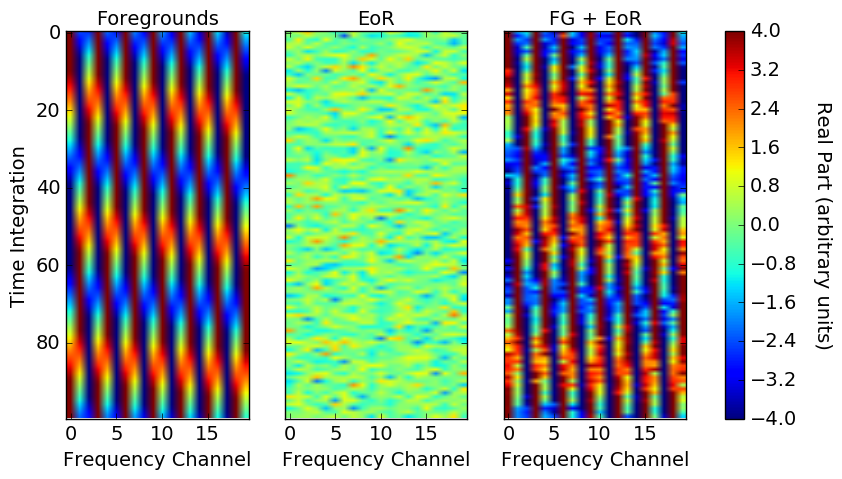
\includegraphics[trim={0cm 0cm 0cm 0cm},clip,width=\columnwidth]{plots/toy_sigloss1.png}
	\caption{Our toy model dataset. We model a mock foreground-only visibility with a sinusoid signal that varies smoothly in 
time and frequency. We model a mock EoR signal as a random Gaussian signal. Real parts are shown here.}
	\label{fig:toy_sigloss1}
\end{figure}

Without a perfect model for the covariance matrix $\textbf{C}$ of our data, one attractive way to estimate it is to empirically derive it from the data $\textbf{x}$ itself (this is what was done in the previous PAPER analyses). For instance, one could time-average such that:

\begin{equation}
\widehat{\textbf{C}} \equiv \langle\textbf{xx}^{\dagger}\rangle_{t},
\end{equation}

\noindent assuming $\langle\textbf{x}\rangle_{t} = 0$ (a reasonable assumption since fringes average to $0$ over a sufficient 
amount of time), where $\langle \rangle_{t}$ denotes a finite average over time. The weighting matrix for estimated inverse covariance weighting is then $
\textbf{R} = \widehat{\textbf{C}}^{-1}$. 

First, we compute the power spectrum of our toy model dataset $\textbf{x}$ using OQE formalism and $\textbf{R} = \widehat{\textbf{C}}^{-1}$. 
The result is shown in green in the left plot of Figure \ref{fig:toy_sigloss3}. Also plotted in the figure are the unweighted ($\textbf{R} = \textbf{I}$) power spectrum of $
\textbf{x}_{FG}$ (blue) and $\textbf{x}_{EoR}$ (red). 

\begin{figure*}
	\centering
	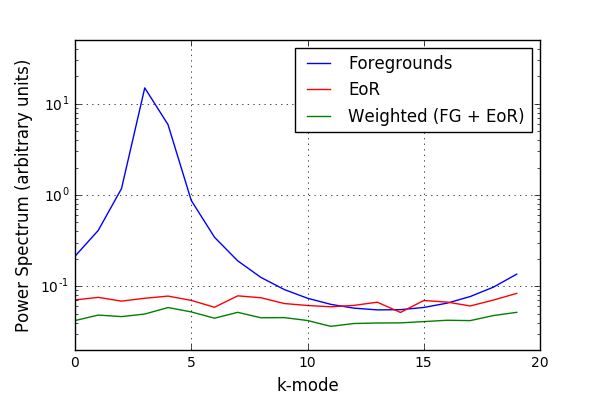
\includegraphics[trim={0cm 0cm 0cm 0cm},clip,height=0.33\textwidth]{plots/toy_sigloss3.png}
	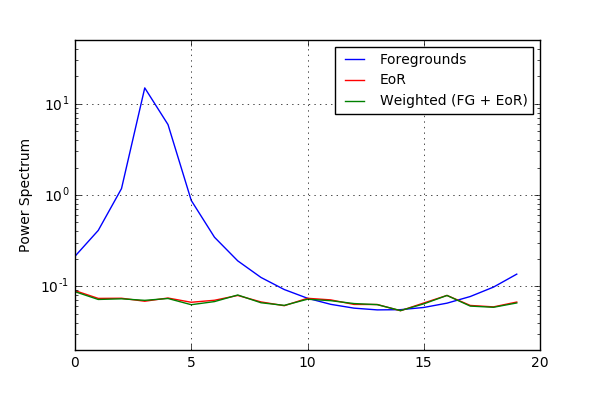
\includegraphics[trim={0cm 0cm 0cm 0cm},clip,height=0.33\textwidth]{plots/toy_sigloss4.png}
	\caption{Resulting power spectrum estimates for the toy model simulation described in Section \ref{sec:toymodel} --- 
foregrounds only (blue), EoR only (red), and the weighted FG + EoR dataset (green). The power spectrum of foregrounds peaks at a $k$ mode based on the frequency of the sinusoid used to create the mock FG signal. In the two panels, we compare inverse covariance weighting 
where $\textbf{C}$ is derived from the data (left), and projecting out the first eigenmode only (right). In the former 
case, signal loss arises from the coupling of the eigenmodes of $\widehat{\textbf{C}}$ to the data. For an empirically estimated $\widehat{\textbf{C}}$, its eigenvalues differ from those of the true covariance, where the weakest (EoR-dominated) eigenmodes are the most strongly coupled to the data and can lead to the most loss.
Hence, there is negligible signal loss when assigning identical weights to all eigenmodes except the first, since we are not using the relative weights of the weaker eigenmodes.}
	\label{fig:toy_sigloss3}
\end{figure*}

As shown, our $\widehat{\textbf{C}}^{-1}$ weighted result successfully suppresses foregrounds. It is also evident that our result fails to 
recover the EoR signal --- it exhibits the correct shape, but the amplitude level is slightly low. This is evidence of signal loss. In short, if the covariance is computed from the data itself, it carries the risk of over-fitting information in the data and introducing a 
multiplicative bias (per $k$) to estimates of the signal. For a toy model mathematical derivation of signal loss arising from a data-estimated covariance matrix, see Appendix \ref{sec:sigloss_appendix}. Here we will describe the origin of this signal loss 
intuitively.

To begin to understand the lossy behavior of this result, we can closely study our estimated covariance eigenspectrum, shown in Figure \ref{fig:toy_sigloss2}. Since it is estimated from our data, its eigenspectrum differs from the eigenspectrum of the true covariance $\textbf{C}$, and this difference has consequences on our result. An eigenspectrum ranks the eigenvalues of a matrix from 
highest to lowest and can be thought of as a spectrum of weights that are given to each spectral mode in the data. In other 
words, the eigenvalues encode the strength of different shapes in the dataset. The eigenspectrum of the identity matrix $
\textbf{I}$ is flat (all $1$'s) because it gives equal weighting to all modes. In our application, covariance matrices tend to have sloped eigenspectra, meaning that modes are given different weights in OQE power spectrum estimation. The modes with the highest eigenvalues are 
down-weighted the most. 

\begin{figure}
	\centering
	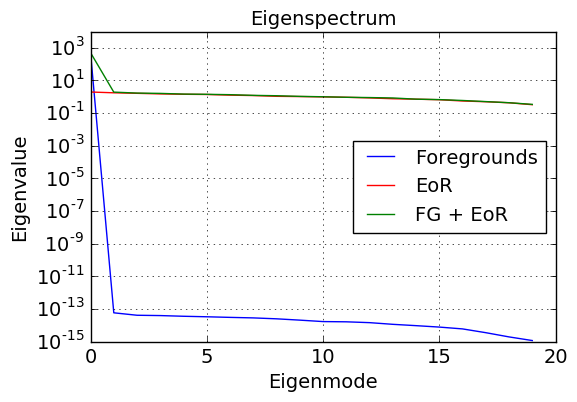
\includegraphics[trim={0cm 0cm 0cm 0cm},clip,width=\columnwidth]{plots/toy_sigloss2.png}
	\caption{Eigenspectrum of $\widehat{\textbf{C}}_{FG}$ (blue), $\widehat{\textbf{C}}_{EoR}$ (red), and $\widehat{\textbf{C}}_{FG+EoR}$ 
(green). The eigenspectrum of $\widehat{\textbf{C}}_{FG}$ peaks at the zeroth eigenmode, due to the presence of only one 
sinusoid. These empirically estimated covariance matrices have eigenspectra that are different from that of a true $\textbf{C}$. Specifically, these eigenmodes have the risk of being down-weighted more significantly than they should be because they are coupled to the data in a way that produces loss.}
	\label{fig:toy_sigloss2}
\end{figure}

Because $\widehat{\textbf{C}}$ is estimated from the data, its eigenvectors and eigenvalues are strongly coupled to the particular data realization that was used to compute it. For example, the strongest mode of $\widehat{\textbf{C}}$ (highest eigenvalue) describes the sinusoid foreground mode in the toy model (the first peak in Figure \ref{fig:toy_sigloss2}). In Figure \ref{fig:toy_sigloss12} we show the covariances of our toy model datasets along with inverse covariance weighted data. The foreground sinusoid is clearly visible in $\widehat{\textbf{C}}_{FG}$.

In general, the strongest eigenmodes of $\widehat{\textbf{C}}$ typically describe bright foregrounds --- the most prominent shapes in a dataset. For these `strong' modes, where foregrounds outshine the EoR signal, down-weighting is beneficial. In some sense, we desire signal loss in this regime, if by `signal' we mean `foregrounds.' In this case it is beneficial for the `strong' eigenmodes to be coupled to the data in a way that produces loss. For our toy model, the successful suppression of the foreground mode is demonstrated in Figure \ref{fig:toy_sigloss2} by the missing foreground peak in the weighted power spectrum estimate (green).

%If the true covariance matrix $\textbf{C}$ of our data was known, then every single eigenvalue and eigenvector of $\textbf{C}$ would be 
%representative of real fluctuations in the data. However, when using an estimated $\widehat{\textbf{C}}$ that is derived from one 
%particular data realization, its eigenvalues and eigenvectors may differ from the truth. Said differently, shapes that may not exist (or exist rarely) in a true covariance may appear stronger in the estimated covariance. Hence, they will be down-weighted 
%more than they should be.

\begin{figure}
	\centering
	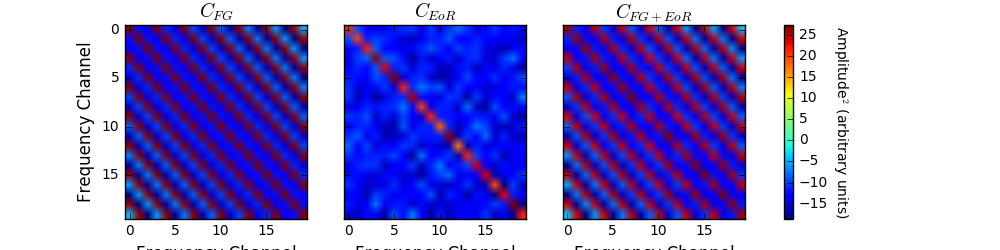
\includegraphics[trim={0cm 0cm 0cm 0cm},clip,width=\columnwidth]{plots/toy_sigloss12.png}
	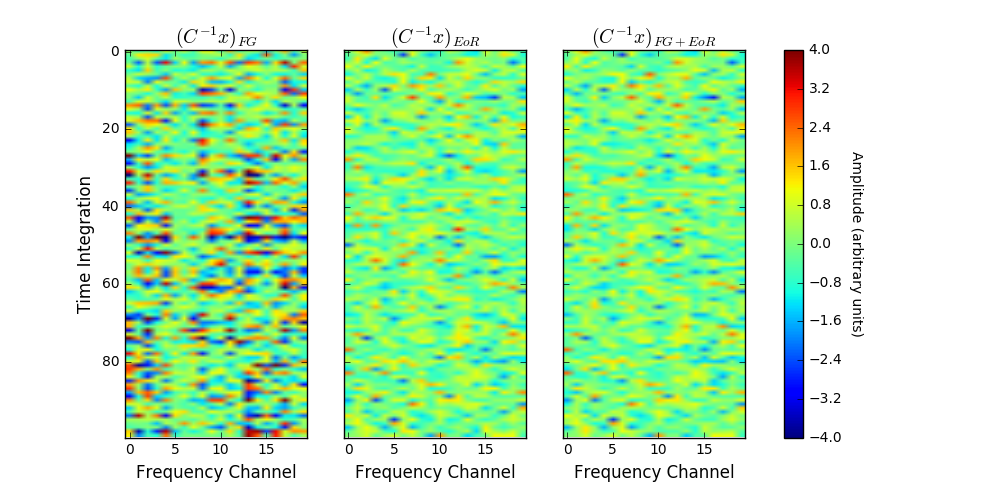
\includegraphics[trim={0cm 0cm 0cm 0cm},clip,width=\columnwidth]{plots/toy_sigloss13.png}
	\caption{The covariance matrices (top row) and inverse covariance-weighted data (bottom row) for FG only (left), EoR only 
(middle), and FG + EoR (right). Real parts are shown here.}
	\label{fig:toy_sigloss12}
\end{figure}

The danger of an empirically estimated covariance matrix comes mostly from not being able to describe the `weak' eigenmodes of $
\textbf{C}$ accurately, for which the EoR signal is brighter than foregrounds. In such a case, the coupling between these modes to the data realization leads to the overfitting and subtraction of the EoR signal. In other words, mis-estimating $\textbf{C}$ for EoR-dominated eigenmodes is more harmful than for FG-dominated modes, and since the `weak' modes of an eigenspectrum are typically EoR-dominated, using this part of the spectrum for weighting is most dangerous.

Using what we've learned about the eigenspectrum, we can tweak it in a simple way to suppress foregrounds and yield minimal 
signal loss. Recall that our toy model foreground is a sinusoid, so it can be perfectly described by a single eigenmode. Using the full dataset's (foreground plus EoR signal) empirical covariance, we can 
project out the first eigenmode and then flatten the rest of the spectrum to have eigenvalues of 1, thereby down-weighting the foreground-dominated mode more than the rest of the modes. Hence, we are changing the weaker part of the spectrum to be less coupled to the data, limiting the amount of over-fitting that can happen for those modes (i.e. only allowing over-fitting to occur for the first mode).

Altering $\widehat{\textbf{C}}$ as such is one specific example of a regularization method for this toy model, in which we are 
changing $\widehat{\textbf{C}}$ in a way that changes its coupling to the data realization. The resulting 
power spectrum estimate for this case is shown in the right plot of Figure \ref{fig:toy_sigloss3}. In this case we recover EoR, 
demonstrating that if we can disentangle the foreground-dominating modes from EoR-dominating modes, we can down-weight 
them with negligible signal loss. There are several other ways to regularize $\widehat{\textbf{C}}$, and we will discuss some in Section 
\ref{sec:otherweight}.

\subsubsection{Toy Model: Fringe-Rate Filtering}
\label{sec:toymodel_frf}

We have shown how signal loss can arise due to the coupling of weak eigenmodes (EoR dominated modes) to the data. We will next show how this effect is exaggerated by reducing the total number of independent 
samples in a dataset. 

A fringe-rate filter is an analysis technique designed to maximize sensitivity by integrating in time (\citealt{parsons_et_al2016}). 
Rather than a traditional box-car average in time, a time domain filter can be designed to up-weight temporal modes consistent with 
the sidereal motion on the sky, while down-weighting modes which are noise-like. 

Because fringe-rate filtering is analogous to averaging in time, it comes at the cost of reducing the total number of independent 
samples in the data. To mimic this filter, we average every four time integrations of our toy model dataset together, yielding 
$25$ independent samples in time (Figure \ref{fig:toy_sigloss5}). We choose these numbers so that the total number of 
independent samples is similar to the number of frequency channels --- our matrices will still be full rank.
%\footnote{If instead we average every $20$ samples together, yielding only $5$ independent samples in time, we are left with a rank deficient covariance matrix. In this case... \cc{fill in}}

The resulting eigenspectrum as compared to the green curve (FG + EoR) in Figure \ref{fig:toy_sigloss2} is shown in Figure 
\ref{fig:toy_sigloss15}. The spectrum, in the case of fringe-rate filtering (dashed line), falls more steeply, especially for 
the last few eigenmodes. In many applications, this steep fall is not indicative of the true covariance structure of the data.

With 
fringe-rate filtering resulting in fewer independent modes, it becomes more difficult for the empirical covariance to estimate the 
true fringe-rate filtered case covariance matrix. This can be quantified by evaluating a convergence metric $\varepsilon(\Chat)$ for the empirical covariance, which we define as
\begin{equation}
\label{eq:converge}
\varepsilon (\Chat) \equiv \sqrt{\frac{\sum_{ij} (\widehat{C}_{ij} - {C}_{ij})^2}{\sum_{ij} {C}_{ij}^2}},
\end{equation}
where $\C$ is true covariance matrix. In Figure \ref{fig:toy_sigloss16} we show this convergence statistic as a function of the number of independent ensemble realizations in one's simulations (horizontal axis) and the number of independent samples in the data following fringe-rate filtering (different curve colors). With more independent time samples (i.e. more realizations) in the data, one converges to the true fringe-rate filtered covariance more quickly. 

The situation here with using a finite number of time samples to estimate our covariance is analogous to a problem faced in galaxy surveys, where the non-linear covariance 
of the matter power spectrum is estimated using a large --- but finite --- number of expensive simulations. There, the limited 
number of independent simulations results in inaccuracies in estimated covariance matrices 
\citep{dodelson_schneider2013,taylor_joachimi_etal2014}, which in turn result in biases in the final parameter constraints 
\citep{hartlap_et_al2007}. In our case, the empirically estimated covariances are used for estimating the power spectrum, and 
as we discussed in the previous section (and will argue more thoroughly in Section \ref{sec:siglossmethod} and Appendix \ref{sec:sigloss_appendix}), couplings between these covariances and the data can lead to power spectrum estimates that are biased 
\emph{low}---which is precisely signal loss. In future work, it will be fruitful to investigate whether advanced techniques from the 
galaxy survey literature for estimating accurate covariance matrices can be successfully adapted for $21\,\textrm{cm}$ 
cosmology. These techniques include the imposition of sparsity priors \citep{padmanabhan_et_al2016}, the fitting of 
theoretically motivated parametric forms \citep{pearson_samushia2016}, covariance tapering \citep{paz_sanchez2015}, 
marginalization over the true covariance \citep{sellentin_heavens2016}, and shrinkage methods 
\citep{pope_szapudi2008,joachimi_2017}.

Just as important as the eigenvalues are the eigenvectors of our empirical covariances. In general, different eigenvectors converge to their true forms at different rates. This is illustrated by Figure \ref{fig:toy_sigloss17}, which shows the convergence of eigenvectors in an empirical estimate of a covariance matrix whose true form is a diagonal matrix with eigenvalues spanning four orders of magnitude. We use as a convergence metric $\varepsilon(\widehat{\textbf{v}})$ for the empirical eigenvectors $\widehat{\textbf{v}}$, defined as:
\begin{equation}
\label{eq:converge_eig}
\varepsilon (\widehat{\textbf{v}}) \equiv \sqrt{\sum_{i}^{N_{f}}|\textbf{v}-\widehat{\textbf{v}}|_{i}^2},
\end{equation}
where $N_{f}$ is the number of frequencies ($20$) in the mock data. The eigenmode convergence curves  in Figure \ref{fig:toy_sigloss17} are ranked ordered by eigenvalue, such that ``Eigenmode \#0" illustrates the convergence of the eigenvector with the largest eigenvalue, ``Eigenmode \#1" for the second largest eigenvalue, and so on. One sees that the stronger eigenmodes converge to their true eigenvectors more quickly. With only a small number of realizations, these empirically estimated modes already retain little correlation with the specific realizations of data that were used to form the empirical covariance. As we will see in the next section, using only the strongest eigenmodes, which are less coupled to data realizations, minimizes signal loss. In contrast, the weaker eigenmodes retain more memory of the data realizations, which leads to correlations that induce signal loss. Said differently, a steep covariance eigenspectrum can be especially dangerous because it is the `weak' modes that are both EoR-dominated and converge the slowest and are therefore susceptible to the most loss.  %\acl{Think about whether we need to do the Fourier space version as well.}

\begin{figure}
	\centering
	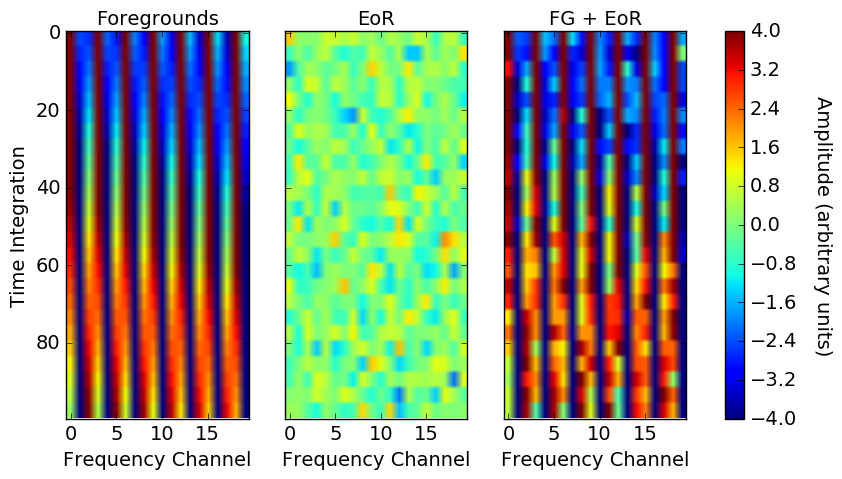
\includegraphics[width=\columnwidth]{plots/toy_sigloss5.png}
	\caption{Our `fringe-rate filtered' (time-averaged) toy model dataset. We average every four samples together, 
yielding $25$ independent samples in time. Real parts are shown here.}
	\label{fig:toy_sigloss5}
\end{figure}

\begin{figure}
	\centering
	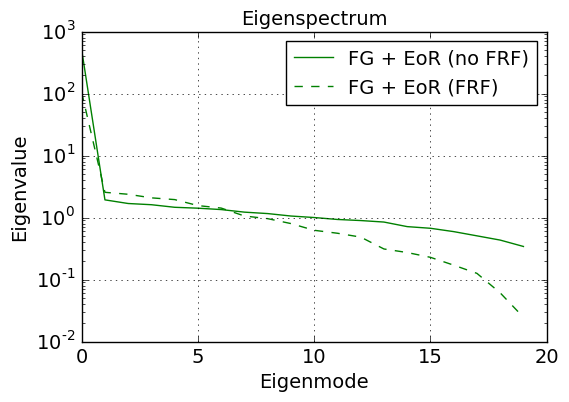
\includegraphics[trim={0cm 0cm 0cm 0cm},clip,height=0.31\textwidth]{plots/toy_sigloss15.png}
	\caption{Eigenspectrum of $\widehat{\textbf{C}}_{FG+EoR}$, in the case of no fringe-rate filtering (solid green) and with fringe-rate filtering (dashed green).}
	\label{fig:toy_sigloss15}
\end{figure}

\begin{figure}
	\centering
	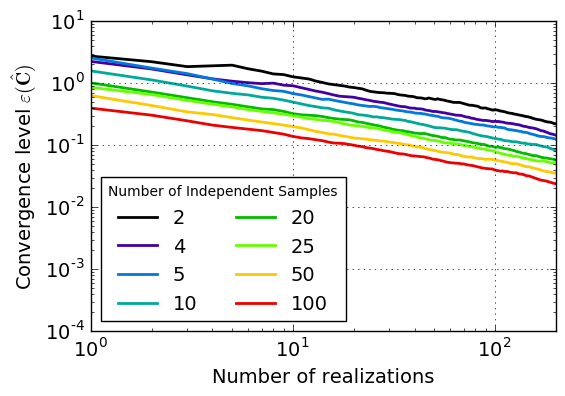
\includegraphics[width=\columnwidth]{plots/toy_sigloss16.png}
	\caption{The convergence level, as defined in Equation \eqref{eq:converge}, of empirically estimated covariances of mock EoR signals with different numbers of independent samples. In red, the mock EoR signal is comprised entirely of independent samples. Subsequent colors show time-averaged signals. As the number of realizations increases, we see that the empirical covariances approach the true covariances. With more independent samples, the quicker an empirical covariance converges, and the less signal loss we would expect to result.}
	\label{fig:toy_sigloss16}
\end{figure}

\begin{figure}
	\centering
	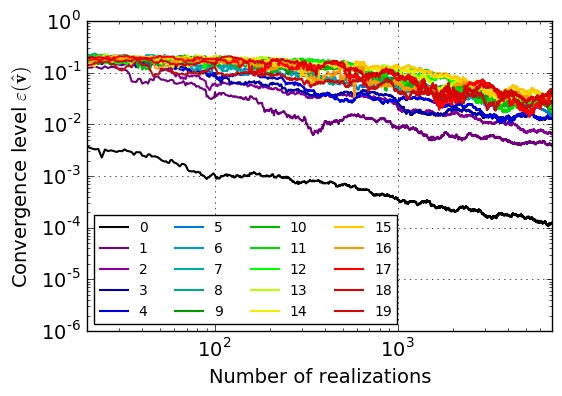
\includegraphics[width=\columnwidth]{plots/toy_sigloss17.png}
	\caption{The convergence level, as defined in Equation \eqref{eq:converge_eig}, of empirically estimated eigenvectors for different number of mock data realizations. The colors span from the 0th eigenmode (the first one) to the 19th eigenmode (the last one), where they are ordered by eigenvalue in descending order. This figure shows that `strong' eigenmodes (those with the highest eigenvalues) converge more quickly than `weak' eigenmodes, implying that weighting by empirically estimated `weak' modes poses the most risk for signal loss.}
	\label{fig:toy_sigloss17}
\end{figure}

\begin{figure}
	\centering
	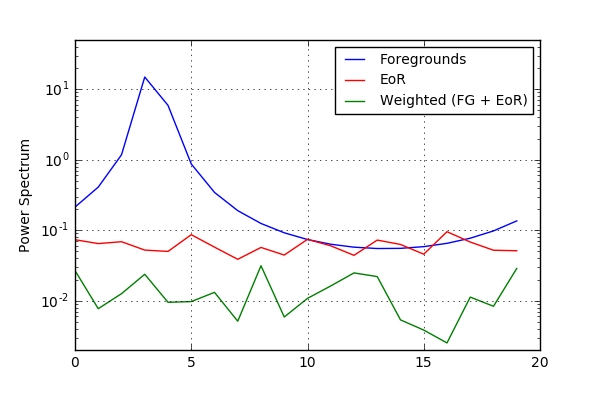
\includegraphics[trim={0cm 0cm 0cm 0cm},clip,width=\columnwidth]{plots/toy_sigloss7.png}
	\caption{Resulting power spectrum estimate for the `fringe-rate filtered' (time-averaged) toy model simulation --- foregrounds only (blue), 
EoR only (red), and the weighted FG + EoR dataset (green). We use inverse covariance weighting where $\textbf{C}$ is 
computed from the data. There is a larger amount of signal loss than for the non-averaged data, a consequence of weighting by empirically estimated eigenmodes that are more strongly coupled to the data due to there being fewer independent modes.}
	\label{fig:toy_sigloss7}
\end{figure}


The power spectrum results for the fringe-rate filtered toy model data is shown in Figure \ref{fig:toy_sigloss7}. As 
expected, there is a much larger amount of signal loss for this time-averaged dataset since we do a worse job estimating the true covariance. In addition, as a result of having fewer independent samples, we obtain an estimate with more scatter. This is evident by noticing that the 
green curve in Figure \ref{fig:toy_sigloss7} fails to trace the shape of the unweighted EoR power spectrum.

Using our toy model, we have seen that a sensitivity-driven analysis technique like fringe-rate filtering has trade-offs of signal 
loss and noisier estimates when using data-estimated covariance matrices. Longer integrations increase sensitivity but reduce 
the number of independent samples, resulting in poorly characterized, steep eigenspectra that can overfit signal greatly. We 
note that a fringe-rate filter does have a range of benefits, many described in \citet{parsons_et_al2016}, so it can still be 
advantageous to use one despite the trade-offs.

\subsubsection{Toy Model: Other Weighting Options}
\label{sec:otherweight}

In Section \ref{sec:toymodel} we showed one example (projecting the zeroth eigenmode) of how altering $\widehat{\textbf{C}}$ can 
make the difference between nearly zero and some signal loss. We will now use our toy model to describe several other ways to tailor $\widehat{\textbf{C}}$ 
in order to minimize signal loss. We choose four independent regularization methods to highlight in this section, which have 
been chosen due to their simplicity in implementation and straightforward interpretations. We illustrate the resulting power 
spectra and eigenspectra for the different cases in Figures \ref{fig:toy_sigloss8} and \ref{fig:toy_sigloss14}. These examples are not meant to be taken as suggested analyses methods but rather as illustrative cases. 

As a first test, we model the covariance matrix of EoR as a proof of concept that if perfect models are known, signal loss can be 
avoided. We know that our simulated EoR signal should have a covariance matrix that mimics the identity matrix, with its 
variance encoded along the diagonal. We model $\textbf{C}_{EoR}$ as such (i.e. the identity), instead of computing it based on $\textbf{x}
_{EoR}$ itself. Next, we add $\textbf{C}_{EoR} + \widehat{\textbf{C}}_{FG}$ (where $\widehat{\textbf{C}}_{FG} = \langle\textbf{x}_{FG}
\textbf{x}_{FG}^{\dagger}\rangle_{t}$) to obtain a final $\widehat{\textbf{C}}$ to use in weighting. In Figure \ref{fig:toy_sigloss8} (upper 
left), we see that there is negligible signal loss. This is because by modeling $\textbf{C}_{EoR}$, we avoid over-fitting EoR fluctuations in the data that our model doesn't know about (but an empirically derived $\widehat{\textbf{C}}$ would). This is also shown by comparing the (steeper) green and (flatter) red curves in Figure \ref{fig:toy_sigloss14}. In practice such a weighting option is not feasible, as it is difficult to model $\textbf{C}_{EoR}$, and $\textbf{C}_{FG}$ is unknown.

\begin{figure*}
	\centering
	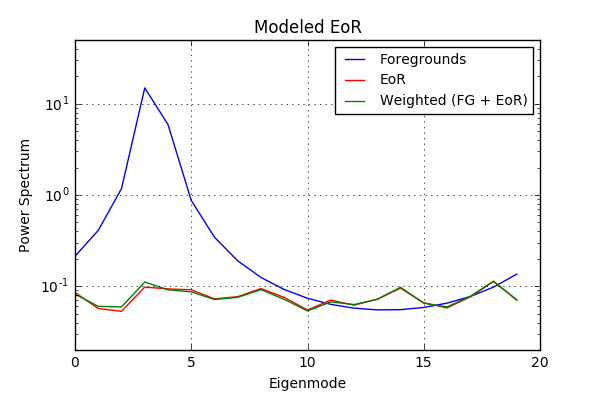
\includegraphics[trim={0cm 0cm 0cm 0cm},clip,height=0.3\textwidth]{plots/toy_sigloss10.png}
	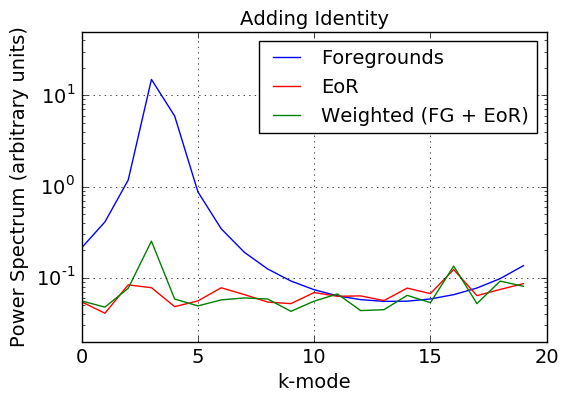
\includegraphics[trim={0cm 0cm 0cm 0cm},clip,height=0.3\textwidth]{plots/toy_sigloss8.png}
	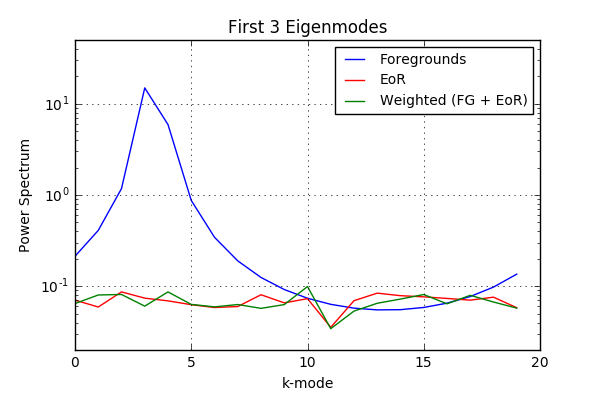
\includegraphics[trim={0cm 0cm 0cm 0cm},clip,height=0.3\textwidth]{plots/toy_sigloss9.png}
	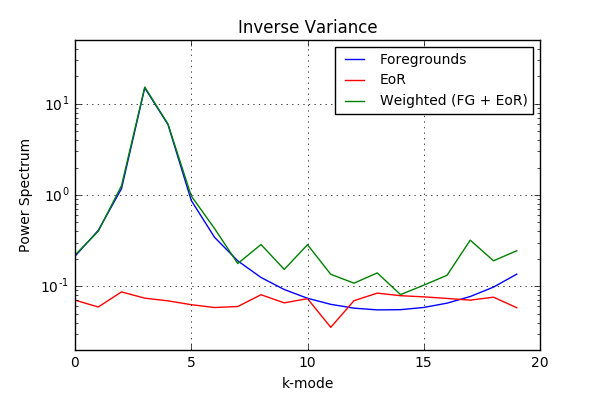
\includegraphics[trim={0cm 0cm 0cm 0cm},clip,height=0.3\textwidth]{plots/toy_sigloss11.png}
	\caption{Resulting power spectra estimates for our `fringe-rate filtered' (time-averaged) toy model simulation --- foregrounds only (blue), 
EoR only (red), and the weighted FG + EoR dataset (green). We show four alternate weighting options that each minimize signal 
loss, including modeling the covariance matrix of EoR (upper left), regularizing $\widehat{\textbf{C}}$ by adding an identity matrix to 
it (upper right), using only the first three eigenmodes of $\widehat{\textbf{C}}$ (lower left), and keeping only the diagonal elements of 
$\widehat{\textbf{C}}$ (lower right). The first case (upper left) is not feasible in practice since we do not know $\textbf{C}_{FG}$ and $\textbf{C}_{EoR}$ like we do in the toy model.}
	\label{fig:toy_sigloss8}
\end{figure*}

\begin{figure}
	\centering
	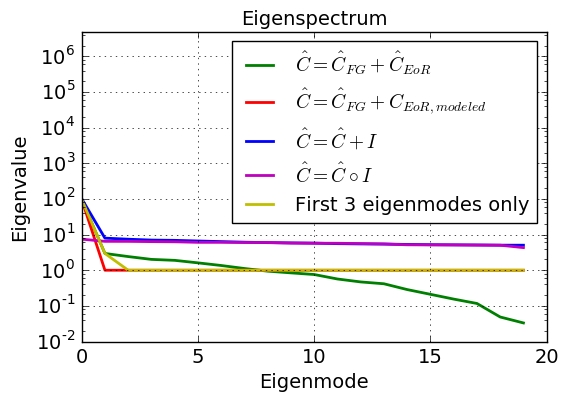
\includegraphics[trim={0cm 0cm 0cm 0cm},clip,width=\columnwidth]{plots/toy_sigloss14.png}
	\caption{We compare the eigenspectrum of an empirically calculated $\widehat{\textbf{C}}$ (green) to that of four alternate 
weighting options, including modeling the covariance matrix of EoR (red), regularizing $\widehat{\textbf{C}}$ by adding an identity 
matrix to it (blue), using only the first three eigenmodes of $\widehat{\textbf{C}}$ (yellow), and multiplying an identity matrix with $
\widehat{\textbf{C}}$ (magenta). All eigenspectra (except the green) are relatively flat and don't exhibit signal loss. All were 
computed for the `fringe-rate filtered' (time-averaged) toy model case presented in Section \ref{sec:toymodel_frf}.}
	\label{fig:toy_sigloss14}
\end{figure}

The second panel (top right) in Figure \ref{fig:toy_sigloss8} uses a regularization method of setting $\widehat{\textbf{C}} = 
\widehat{\textbf{C}} + \gamma\textbf{I}$, where $\gamma = 5$ (an arbitrary strength 
of $\textbf{I}$ for the purpose of this toy model). By adding the identity matrix, element-wise, we are weighting the diagonal 
elements of the covariance matrix more heavily than those off-diagonal. Since the identity component does not know anything about the data realization, it alters the covariance to be less coupled to the data. Although there is negligible signal loss using this regularization, the small green peak at $k\sim3$ represents residual foregrounds that still exist since the shapes encoded in the off-diagonal frequency correlations of the covariance matrix were deemed not as prominent as the diagonal elements using this weighting scheme. 

The third panel (bottom left) in Figure \ref{fig:toy_sigloss8} minimizes signal loss a different way - 
by only using the first three eigenmodes of the estimated covariance. Recalling that our toy model foregrounds can be described entirely by the first eigenmode, this 
method intentionally projects out modes that are EoR-dominated by replacing all but the three highest weights in the 
eigenspectrum with $1$'s (equal weights). Again, avoiding the over-fitting of `weak' modes which are coupled to the data results in negligible signal loss. However, we do 
not perfectly recover the shape of EoR because we lost information when projecting out certain modes. While this case is illuminating for the toy model, in practice it is not obvious which eigenmodes are FG vs. EoR dominated, so selecting a subset of modes to down-weight is not trivial. 

The last regularization scheme we are highlighting here is setting $\widehat{\textbf{C}} = \widehat{\textbf{C}} \circ \textbf{I}$ (element-wise multiplication), or inverse variance weighting (keeping only the diagonal elements of $\widehat{\textbf{C}}$). In the bottom right 
panel of Figure \ref{fig:toy_sigloss8}, we see that this method does not down-weight the foregrounds --- this regularization altered $\widehat{\textbf{C}}$ in a way where it's no longer coupled to both the `strong' or `weak' eigenmodes. For this toy model, 
our foregrounds are spread out in frequency and therefore have non-negligible frequency-frequency correlations. Multiplying by 
the identity, element-wise, results in a diagonal matrix, meaning we are only left with correlation information between the same 
two frequencies. Because we disregard information from all other frequency combinations in this case, we do a poor job 
suppressing the foreground. But because we de-coupled the whole eigenspectrum from the data, we also avoid signal loss. Although this method did not successfully recover EoR for this particular simulation, it is important that we show that there 
are many options for estimating a covariance matrix, and some may down-weight certain eigenmodes more than others based on the spectral nature 
of the components in a dataset. 
%One may imagine a situation where a particular systematic is contained to an isolated 
%frequency (such as radio frequency interference or crosstalk). In such a case, preserving only the diagonal elements of $
%\widehat{\textbf{C}}$ would be an effective way of removing this contamination. 

In summary, we have a choice of how to weight $21$ cm data. Ideally, we want to down-weight bright foregrounds without 
removing the underlying cosmological signal. However, there are trade-offs between the weighting method 
used, its foreground-removal effectiveness, the number of independent samples in a dataset, and the amount of resulting signal loss. 

% SECTION 2 ERROR ESTIMATION ---------------------------------------------------------------------------------

\subsection{Error Estimation}
\label{sec:ErrorOverview}

Our second major $21$ cm power spectrum theme is error estimation, as we desire robust methods for determining accurate 
confidence intervals for our measurements. Two popular ways of calculating errors on a power spectrum 
measurement are calculating the variance of a dataset, and computing a theoretical error estimate based on an instrument's 
system temperature and observational parameters. In a perfect world, both methods would match up. However, in practice the 
two don't always agree due to a number of factors, including possible non-Gaussianities in the noise properties of our instruments and non-uniform 
weightings. 

For PAPER's analysis, we choose to compute error bars that have been derived from the inherent 
variance of our measurements. A common technique used to do this is bootstrapping. For pedagogical purposes, we first define the technique of 
bootstrapping and then illustrate one of its pitfalls through a toy model.

Bootstrapping uses sampling with replacement to estimate a posterior distribution. For example, measurements (like power 
spectra) can be made from different samples of data. Each of these measurements is a different realization drawn from some underlying distribution, and realizations are correlated with each other to a degree set by the fraction of sampled points that are held in common 
between them. Through the process of resampling and averaging along different axes, we can estimate error bars for 
our results which represent the underlying distribution of values that are allowed by our measurements (\citealt{efron_tibshirani1994}; \citealt{andrae2010}).

Suppose we have $N$ different measurements targeting the same quantity ($N$ power spectrum measurements made along different axes, such as baselines or times). 
Bootstrapping means that we form $N_{boot}$ (often a large number) bootstraps, where each bootstrap is a random selection 
of the $N$ measurements. Bootstraps each have dimensions of $N$, and the values populated into each bootstrap are drawn 
from the original set of measurements with replacement (i.e. every $n^{th}$ slot in $N$ is filled randomly for each bootstrap). Next we take 
the mean of each bootstrap to collapse it from an array of length $N$ to a single number (we are interested in the mean statistic 
here, but any function of interest can be applied to each bootstrap as long as it's the same function for each one). The error (on 
the mean) is then computed as the standard deviation across all bootstraps. 

We must be careful in distinguishing $N_{boot}$, the number of bootstraps, from $N$, the number of samples, or elements, or 
values, that comprise a bootstrap. In the toy models presented in this section, $N_{boot}$ is typically large, and the standard 
deviation across bootstraps (the error we are computing) converges for large $N_{boot}$. Typically $N$ is a straightforward value to set that just depends on the experiment. However, we will illustrate one case in which it is not simply the number of samples along the axis that is being re-sampled. More specifically, we will see that $N$ depends on sample independence and may not always be straightforward to approximate. 

For our toy model, suppose we have a Gaussian random signal dataset of length $N=1000$ and unity variance (zero mean). 
This could represent $1000$ power spectrum measurements, for which we are interested in its error. We predict that the error 
on the mean should obey $1/\sqrt{N}$, where $N$ is the number of samples.

We next form $500$ bootstraps ($N_{boot} = 500$). To create each bootstrap, we draw $N$ samples, with replacement, of the 
original data, and take the mean over the $N$ samples. The standard deviation over the $500$ bootstraps gives an error 
estimate for our dataset. This error is indicated by the gray star in Figure \ref{fig:toy_error1} and matches our theoretical 
prediction (green).

One major caveat of bootstrapping arises when working with correlated data. If, for example, a dataset has many repeated 
values inside it, this would be reflected in each bootstrap. The same value would be present multiple times within a bootstrap 
and also be present between bootstraps, purely because it has a more likely chance of being drawn if there are repeats of 
itself. Therefore, bootstrapping correlated data results in a smaller variation between bootstraps, and hence, under-estimates 
errors. The use of a fringe-rate filter, which averages data in time to increase sensitivity, is one example which leads to a 
reduction in the number of independent samples, creating a situation in which errors can be under-estimated. We will now show 
this effect using our toy model.

Going back to our toy model, we apply a sliding boxcar average to $10$ samples at a time, thus reducing the number of 
independent data samples to $N/10 = 100$. Bootstrapping this time-averaged noise, using the same method as described 
earlier (drawing $N$=$1000$ elements per bootstrap sample), under-estimates the error by a factor of $\sim3$ (black points in Figure \ref{fig:toy_error1}, at $N$=$1000$). This occurs 
because we are drawing more samples than independent ones available, and thus some samples are repeated multiple times 
in all bootstraps, leading to less variation between the bootstraps. In fact, the error derived from bootstrapping is a strong 
function of the number of elements that are drawn per bootstrap (Figure \ref{fig:toy_error1}, black points), and we can both 
under-estimate the error by drawing too many or over-estimate it by drawing too few. However, since we know that we have $100$ 
independent samples in this toy model, the error associated with drawing $N$=$100$ samples with replacement does match the theoretical prediction 
as expected (the black points cross the green line at $N$=$100$ in Figure \ref{fig:toy_error1}).

This example highlights the importance of understanding how analysis techniques (e.g. fringe-rate filtering) can affect a 
common statistical procedure like bootstrapping. Bootstrapping as a means of estimating power spectrum errors from real 
fringe-rate filtered data requires knowledge of the number of independent samples, which is not always a trivial task. For 
example, computing the effective number of independent samples of fringe-rate filtered data is not as simple as counting the 
number of averages performed. Down-sampling a time-averaged signal is straightforward using a boxcar average, but non-trivial with a more complicated convolution function that has long tails. Hence, we do not recommend bootstrapping unless the 
number of independent samples along the axis that is being re-sampled is well-determined. In Section \ref{sec:Boot}, we explain how our bootstrapping procedure has changed in PAPER's analysis in light of this issue. 

\begin{figure}
	\centering
	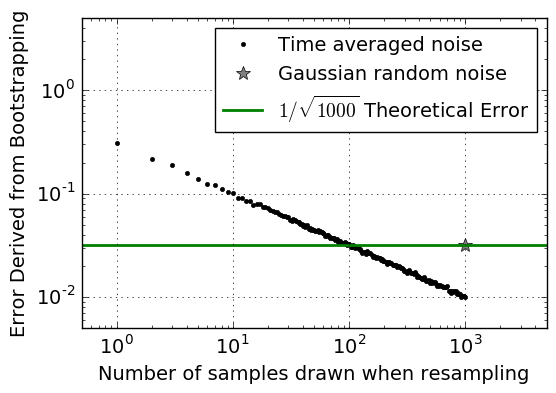
\includegraphics[trim={0cm 0cm 0cm 0cm},width=\columnwidth]{plots/toy_error1.png}
	\caption{Error estimation from bootstrapping as a function of the number of elements drawn per bootstrap when 
sampling with replacement. The star represents the standard deviation of $N_{boot}=500$ bootstraps, each created by drawing $1000$ 
elements (with replacement) from a length $1000$ array of a Gaussian random signal. The black points correspond to time-averaged data (correlated data) which has $100$ independent samples. They illustrate how errors can be under-estimated if 
drawing more elements than there are independent samples in the data. The estimated errors match up with the theoretical 
prediction only at $N=100$.}
	\label{fig:toy_error1}
\end{figure}

\begin{comment} % REMOVED THIS HALF OF BOOTSTRAPPING SECTION
We will now discuss a second subtle feature of bootstrapping that fails to maximize the sensitivity of a dataset. Suppose we 
have $5$ independent measurements of the sky (from $5$ different baselines, for example). A bootstrap then consists of $5$ 
measurements that are drawn randomly with replacement from the original set. If all $5$ spaces are filled randomly, there is a 
high probability that some measurements will be repeated in the bootstrap because they are drawn more than once. The 
bootstrap may therefore consist of only $3$ or $4$ independent measurements --- a number smaller than the total number of 
samples. In fact, the probability of drawing $5$ completely independent measurements is less than $4\%$.

In order to maximize sensitivity, we desire as many independent samples as possible. However, solely using all $5$ 
independent measurements does not allow variation between bootstraps. 

Therefore, we use a slightly modified bootstrapping method. For each bootstrap, we draw $N-1=4$ samples without 
replacement and draw the last slot randomly with replacement. In doing so there is a small chance a bootstrap will consist of 
$5$ independent measurements, but even with $4$ our sensitivity is nearly maximized. 
%One may wonder whether this change is still a legitimate way of error estimating since random sampling only occurs for one value in a bootstrap. However, as long as the number of possible variations is greater than the number of bootstraps we perform, it is a valid way to uncover the inherent variability in a dataset. 

In Figure \ref{fig:toy_error2} we compare these two methods of bootstrapping: sampling all elements randomly (black points) 
versus sampling just the final element randomly (gray points). The two converge for datasets with small numbers of elements, 
when filling a few spots randomly is nearly the same as filling only the last spot randomly. However, there is also increased 
scatter in this regime due to small number statistics. 

The difference between the two methods is most pronounced for datasets with large numbers of elements. As a dataset grows 
in size, it becomes increasingly rare to draw entirely independent samples, and thus the benefit of ensuring, say, $999$ 
independent samples out of $1000$ is most noticeable. The more elements in our dataset, the more sensitivity we can gain by 
mandating that most of our measurements are independent ones. An analog for the y-axis in Figure \ref{fig:toy_error2} is 
therefore the sensitivity of a final power spectrum measurement.
\end{comment}

In summary, bootstrapping can be an effective and straightforward way to estimate errors of a dataset. However, we have 
illustrated a situation in which bootstrapping can lead to under-estimated errors and therefore under-estimated power spectrum limits. We have shown that 
bootstrapped error depends strongly on the number of elements drawn in a bootstrap sample. Estimated errors can drop to 
arbitrarily small values when the number of elements drawn exceeds the effective number of independent elements. 
%We have also shown a situation in which a bootstrapping method does not provide the most sensitive measurement possible. 
While bootstrapping is convenient because it provides a way to estimate errors from the data itself, one must assess whether certain 
analysis choices have compromised the method and whether a variation or an avoidance of traditional re-sampling could be preferred instead.

%\begin{figure}
%	\centering
%	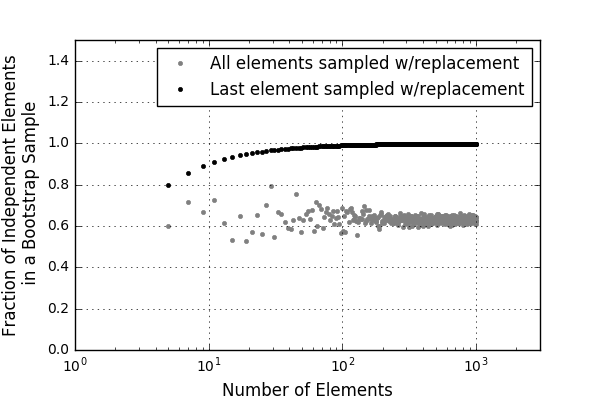
\includegraphics[trim={0cm 0cm 0cm 0cm},width=\columnwidth]{plots/toy_error2.png}
%	\caption{The fraction of independent elements in one bootstrap sample as a function of the total number of elements in a 
%dataset (i.e. if $4$ out of $5$ elements are independent, this would yield a fraction of $0.8$). A fraction of $1.0$ means that all 
%elements in the bootstrap sample are independent, and therefore sensitivity is maximized (alternately, this axis can be thought 
%of as power spectrum sensitivity, where sensitivity increases moving upwards along the y-axis). Two bootstrapping methods are shown here --- sampling all elements with replacement (gray) and sampling only the last element with replacement (black). The former fails to maximize sensitivity since some elements end up being repeated due to random sampling.} 
%The `outlier' points lying at a fraction of $1.0$ at the far left of the plot occur in the off-chance that the last spot in the sample happens to be the one missing element instead of a repeated element --- this is more likely to happen with a small total number of elements but also results in a more dramatically different fraction as compared to the case of a repeated element in the last spot, hence why these points appear like outliers.}
%	\label{fig:toy_error2}
%\end{figure}

% SECTION 2 BIAS ---------------------------------------------------------------------------------

\subsection{Bias}
\label{sec:BiasOverview}

In a $21$ cm power spectrum, detections could be the EoR signal, but they could also 
%(and unfortunately more likely) 
be attributed to other sources of bias. Connecting a detection to EoR as opposed to noise or foreground bias is a key challenge of 
future $21$ cm data analyses \citep[e.g.][]{petrovic_and_oh2011}. In this section we will discuss possible sources of bias in a measurement, as well as techniques 
that can help mitigate their effects. We will also present a series of tests in a pedagogical fashion which we suggest be used to 
help evaluate deep limits and/or detections.

\subsubsection{Foreground and Noise Bias}
\label{sec:BiasTypes}

In Section \ref{sec:SiglossOverview}, we discussed signal loss as a form of multiplicative bias to estimates of the signal. Foregrounds are another type of bias, but an additive one instead of multiplicative. Foreground bias is perhaps one of the main factors limiting $21$ cm results, as foreground signals lie $\sim4$-$5$ orders of 
magnitude above the cosmological signal. Though there are many techniques proposed for removing foregrounds (see e.g. \citealt{vedantham_et_al2012}; \citealt{parsons_et_al2012a}; \citealt{parsons_et_al2012b}; \citealt{dillon_et_al2013a}; \citealt{wang_et_al2013}; \citealt{parsons_et_al2014}; \citealt{liu_et_al2014a}; \citealt{liu_et_al2014b}; \citealt{dillon_et_al2015}; \citealt{pober_et_al2016a}; \citealt{trott_et_al2016}), most 
experiments currently remain limited by residuals rather than noise, especially at low $k$.

For a particular 
baseline length, there is a maximum delay imposed on sources attached to the sky, which corresponds to the light-crossing time between two 
antennas in a baseline. For longer baselines, this value increases, producing what is known as ``the 
wedge"
\citep{datta_et_al2010, parsons_et_al2012b, vedantham_et_al2012, pober_et_al2013, thyagarajan_et_al2013, liu_et_al2014a, liu_et_al2014b, patil_et_al2017}. 
The wedge describes a region in $k$-space contaminated by smooth spectrum foregrounds, bounded by baseline length (which is proportional to $k_{\perp}$) and delay (which is 
proportional to $k_{\parallel}$). Properties of the wedge can be used to isolate and 
%remove 
avoid foregrounds, as done by A15, 
\citet{parsons_et_al2014}, \citet{dillon_et_al2014}, \citet{dillon_et_al2015}, \citet{jacobs_et_al2015}, \citet{beardsley_et_al2016}, and \citet{trott_et_al2016}.

Although smooth spectrum foregrounds preferentially show up at low delay, or low $k$ modes, their isolation within the wedge is not perfect. In deep measurements, power spectrum measurements at $k_{\parallel}$ values beyond 
the delay associated with the length of a baseline are often still contaminated at a low level. This leakage, particularly at low $k$'s, can be attributed to 
convolution kernels associated with Fourier-transforming visibilities into delay-space. In other words, smooth-spectrum 
foregrounds appear as $\delta$-functions in delay-space, convolved by the Fourier transform of the source spectrum, the signal chain, and the 
antenna response, all of which could smear out the foregrounds and cause leakage outside the wedge \citep[e.g.][]{ewall-wice_et_al2017}.

There are analysis techniques to mitigate the effects of foreground leakage and prevent information from low $k's$ from 
spreading to high $k$ values. For example, narrow window functions in delay-space can be used to minimize the leakage from a particular 
$k$ value into other ones (\citealt{liu_et_al2014b}). In other words, one can construct an estimator using OQE that forces a 
window function to have a minimum response to low $k$ values. The window function used in A15 is constructed in such a way, 
specifically to prevent foregrounds that live at low $k's$ from contaminating higher $k$-modes (see Section \ref{sec:Bias}). 

Determining the source of positive non-EoR detections at higher $k$'s is more difficult. In previous power spectrum results, these detections have been explained as instrumental systematics, particularly time-variable cross talk, RFI, cable reflections, and calibration errors (A15; \citealt{parsons_et_al2014}; \citealt{dillon_et_al2014}; \citealt{beardsley_et_al2016}; \citealt{patil_et_al2017}). In the next section (Section \ref{sec:JackknifeOverview}), we will present some tests that can help distinguish these excesses from that of EoR. 

In addition to foreground bias, noise can also be responsible for positive power spectrum detections if thermal noise is 
multiplied by itself. Every $21$ cm visibility measurement contains thermal noise that is comprised of receiver and sky noise. 
We expect this noise to be independent between antennas and thus we can beat it down (increase sensitivity) by integrating 
longer, using more baselines, etc. However, the squaring of noise occurs when cross-multiplying visibilities, which is shown by 
the two copies of $\textbf{x}$ in Equation \eqref{eq:qhat}. If both copies of $\textbf{x}$ come from the same baseline and time, it 
can result in power spectrum measurements that are higher than those predicted by the thermal noise of the instrument. One 
way to avoid this type of noise bias is to avoid cross-multiplying data from the same baselines or days. This ensures that the 
two quantities that go into a measurement have separate noises that don't correlate with each other. We also note that if the noise level is known, this type of bias can be subtracted off, though this procedure is argued to be dangerous by \citet{dillon_et_al2014}.

Another type of noise bias can stem from the spurious cross-coupling of signals between antennas. This excess is known as 
instrumental crosstalk and is an inadvertent correlation between two independent measurements via a coupled signal path. 
Crosstalk appears as a constant phase bias in time in visibilities, and it varies slowly compared to the typical fringe-rates of 
sources. Because it is slow-varying, crosstalk can be suppressed using time-averages or fringe-rate filters. However, there 
remains a possibility that power spectrum detections that aren't the cosmological signal are caused by residual, low-level crosstalk which survived any 
suppression techniques. 

\subsubsection{Jackknife Tests}
\label{sec:JackknifeOverview}

We now approach the difficult task of tracing excesses to foreground, noise, and EoR biases through a discussion of useful 
jackknife tests. Again, we first approach this topic pedagogically as an introduction to the related PAPER discussion in Section 
\ref{sec:Bias}. 

The jackknife is a resampling technique in which a statistic (i.e. power spectrum) is computed in subsets of the data (\citealt{quenouille1949}; \citealt{tukey1958}). These 
subsets are then compared to reveal systematics. In this section we define two main tests --- the null test and the traditional 
jackknife --- and explain how a power spectrum detection must pass each. We then highlight how these tests can be used to 
help distinguish between different sources of bias.
 
\begin{itemize}
\item \textbf{Null Test}: A null test is a type of jackknife test that removes the astronomical signal from data in order to 
investigate underlying systematics (e.g., see \citet{keating_et_al2016} for examples from intensity mapping that are closely related to our current application). For example, one can 
divide data into two subsets by separating odd and even Julian dates, or the first half of the observing season from the second. 
Subtracting the two removes signal that is common to both subsets, including foregrounds and EoR. The resulting power 
spectrum should be consistent with thermal noise estimates; if it is not, it suggests the presence of a systematic that differs 
from one of the data subsets to the other (i.e. doesn't get subtracted perfectly). 
\item \textbf{Traditional Jackknife}: In a broader sense, it is important to perform many jackknife tests in order to instill 
confidence in a final result. A stable result must be steadfast throughout all jackknives no matter how the data is sliced. 
Jackknives can be taken along several different axes --- for example, one could start with a full dataset, and compute a new 
power spectrum every time as a day of data is removed, or a baseline is removed. This type of jackknife would reveal bias 
present only at certain LSTs (such as a foreground source), for example, or misbehaving baselines.
\end{itemize}

While the null test hunts for deviations from thermal noise and the jackknife tests for deviations in subsamples, they are both 
closely related. We can highlight the connection between the two using a toy model dataset.

Suppose we have two measurements (for example, from two baselines), $\textbf{x}_{a}$ and $\textbf{x}_{b}$. The 
measurements have dimensions of $200$ time integrations and $20$ frequency channels. They each have separate thermal 
noises constructed as a Gaussian random signal for each, and identical EoR signals. 

To mimic the presence of a systematic in part of the measurement, we add a toy sinusoid foreground, similar to the one used in 
Section \ref{sec:toymodel}, to the first $100$ time integrations of both measurements. This represents a foreground signal 
present in, for example, the first half of the LST range used for analysis, but not the second half. Mathematically, if  $\textbf{n}$ 
is noise, $\textbf{e}$ is the EoR signal, and $\textbf{f}$ is the foreground signal, the two measurements (which are cross-multiplied to form power spectra) can be written as:

\begin{equation}
\label{eq:bias1}
\textbf{x}_{a} = \textbf{n}_{a} + \textbf{e} + \textbf{f}
\end{equation} 

\noindent and 

\begin{equation}
\label{eq:bias2}
\textbf{x}_{b} = \textbf{n}_{b} + \textbf{e} + \textbf{f}.
\end{equation}

\noindent The two jackknife samples are $\textbf{x}_{1}$ and $\textbf{x}_{2}$, representing jackknives in time. These can be 
written (for both measurements $a$ and $b$) as:

\begin{eqnarray}
\textbf{x}_{1} &=& \textbf{n} + \textbf{e} + \textbf{f} \\
\textbf{x}_{2} &=& \textbf{n} + \textbf{e} 
\end{eqnarray}

\noindent For example, $\textbf{x}_{1a}$ represents a jackknife sample (first half of the data) for the first measurement. 
Similarly, $\textbf{x}_{2b}$ represents a jackknife sample (second half of the data) for the second measurement.

We do not perform a time-average or apply a fringe-rate filter to this toy model, since we are interested only in what jackknife 
tests can tell us about biases. For the same reason, we use a weighting matrix of $\textbf{I}$ for power spectrum estimation to 
avoid signal loss. 

We form three different power spectrum estimates shown in Figure \ref{fig:toy_bias1}. The first is a null test where we subtract $
\textbf{x}_{2}$ from $\textbf{x}_{1}$ for both measurements $a$ and $b$. This is equivalent to splitting up a full dataset along 
an axis (in this case, time) and subtracting the two to remove sky signal that should ideally be present in both. We cross-multiply measurements $a$ and $b$ to form an un-biased (thermal noise-wise) estimate (blue curve). The second estimate, 
shown in red, is the same null test with the foreground systematic removed (eliminate $\textbf{f}$ in Equations \ref{eq:bias1} 
and \ref{eq:bias2}). Finally, we also show the noise power spectrum (green).

From this test we see a clear difference between the null test with the presence of the foregrounds, and the power spectrum of 
noise. This signifies a non-EoR bias that is only present in either $\textbf{x}_{1}$ or $\textbf{x}_{2}$, but not both.

\begin{figure}
	\centering
	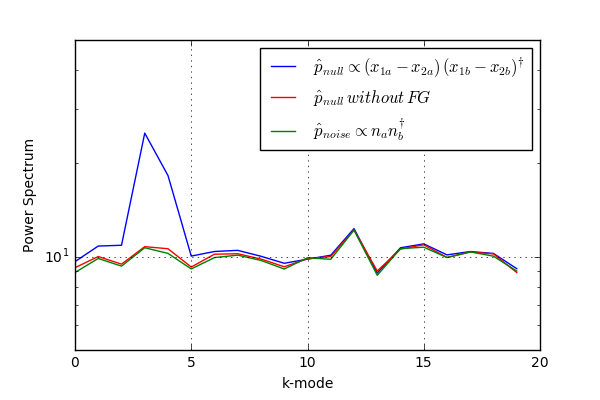
\includegraphics[trim={0cm 0cm 0cm 0cm},width=\columnwidth]{plots/toy_bias1.png}
	\caption{Power spectrum estimates for a null jackknife test with the presence of a foreground systematic (blue), without 
the foreground systematic (red), and noise alone (green). Because the first null test is not consistent with noise, it suggests the 
presence of a systematic in either $\textbf{x}_{1}$ or $\textbf{x}_{2}$. Null tests of clean measurements should be consistent 
with thermal noise.}
	\label{fig:toy_bias1}
\end{figure}

\begin{figure}
	\centering
	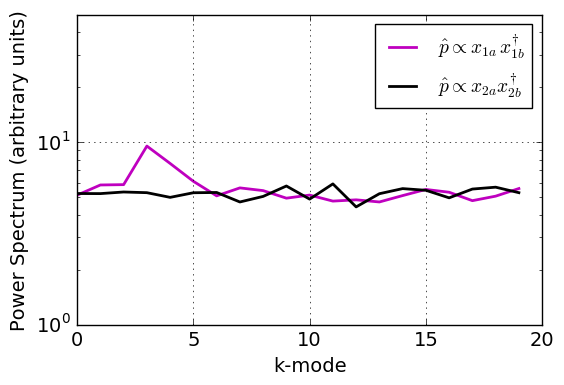
\includegraphics[trim={0cm 0cm 0cm 0cm},width=\columnwidth]{plots/toy_bias2.png}
	\caption{Power spectrum estimates for $\textbf{x}_{1}$ and $\textbf{x}_{2}$, two jackknives of the toy model. They suggest 
the presence of a systematic in $\textbf{x}_{1}$ only (which is exactly what was put in), illustrating how jackknives can be used to tease out excesses. Clean 
measurements should remain consistent despite the jackknife taken.}
	\label{fig:toy_bias2}
\end{figure}

While the null test is useful for testing noise properties and the uniformity of a dataset, jackknives are useful in pinpointing 
which data subsets are contaminated by biases and which are not; in our toy model we see that the bias exists only in $
\textbf{x}_{1}$ (Figure \ref{fig:toy_bias2}). If foreground or noise biases exist in a dataset, jackknives can tease them out and 
provide insight into possible sources. For example, if jackknives along the time-axis reveal a bias present at a certain LST, a 
likely explanation would be excess foreground emission from a radio source in the sky at that time. A jackknife test involving 
data before and after the application of a fringe-rate filter can reveal whether cross-talk noise bias is successfully suppressed 
with the filter, or if similar-shaped detections in both power spectra suggest otherwise. There are many other jackknife axes of 
which we will not go into detail here, including baseline, frequency, and polarization. Ultimately, an EoR detection should persist 
through them all and a clean measurement should exhibit noise-like null spectra.

In this section we have highlighted how null tests and jackknife tests are key for determining the nature of a power spectrum 
detection. In Section \ref{sec:Bias} we perform some examples of these tests on PAPER-64 data in order to prove that our 
excesses are not EoR and to identify their likely cause. 

% SECTION 3  ---------------------------------------------------------------------------------

\section{Demonstration in PAPER-64 Data}
\label{sec:CaseStudy}

In the previous sections we have discussed three overarching $21$ cm power spectrum themes --- signal loss, error estimation, 
and bias. Understanding the subtleties and trade-offs involved in each is necessary for an accurate and robust understanding of 
a power spectrum result. 

We now apply these lessons to data from the PAPER experiment to make a new analysis of the PAPER-64 dataset originally presented in 
A15 and obtain a revised power spectrum estimate.

As a brief review, PAPER is a dedicated $21$ cm experiment located in the Karoo Desert in South Africa. The PAPER-64 
configuration consists of 64 dual-polarization drift-scan elements that are arranged in a grid layout. For our case study, we 
focus solely on Stokes I estimated data \citep{moore_et_al2013} from PAPER's $30$ m East/West baselines (Figure 
\ref{fig:ant_layout}). All data is compressed, calibrated (using self-calibration and redundant calibration), delay-filtered (to remove foregrounds inside the wedge), LST-binned, and fringe-rate filtered. For detailed information about the backend system of PAPER-64, its observations, and data reduction pipeline, we 
refer the reader to \citet{parsons_et_al2010} and A15. We note that all data processing steps are identical to those in A15 until after the LST-binning step in Figure 3 of A15.

\begin{figure}
	\centering
	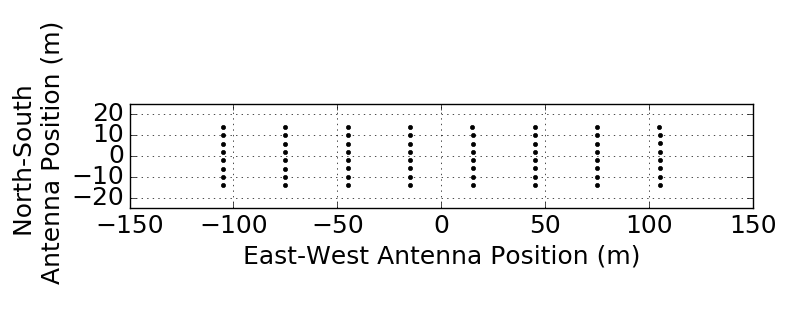
\includegraphics[trim={0cm 0cm 0cm 0cm},width=\columnwidth]{plots/ant_layout_aspect.png}
	\caption{The PAPER-64 antenna layout. We use only the $30$ m East/West baselines for the revised analysis in this 
paper (i.e. the shortest horizontal spacings).}
	\label{fig:ant_layout}
\end{figure}

The previously best published $21$ cm upper limit result from A15 uses $124$ nights of data to place a $2\sigma$ upper limit 
on $\Delta^{2}(k)$, defined as

\begin{equation}
\Delta^{\textbf{2}}(k) = \frac{k^{3}}{2\pi^{2}}\widehat{\textbf{p}}\textbf{(k)},
\end{equation}

\noindent of $(22.4$ mK$)^{2}$ in the range $0.15 < k < 0.5$ h Mpc$^{-1}$ at $z = 8.4$. The revision of this limit (Kolopanis et al., \textit{in prep}) stems from previously underestimated signal loss and underestimated error bars, both of which we 
address in the following sections. 

For our analysis, we use $8.1$ hours of LST (RA $0.5$-$8.6$ hours) and $51$ total baselines (A15 uses a slightly different RA 
range of $0$-$8.6$ hours). All power spectrum results are produced for a center frequency of $151$ MHz using a width of $10$ 
MHz ($20$ channels), identical to the analysis in A15. We note that, besides using only one baseline type instead of the three as in 
A15, the PAPER-64 dataset that we use in this case study differs from that in A15 only in the analysis. The most significant changes occur in the power spectrum analysis, which is explained in the rest of this paper, but we also note that the applied fringe-rate filter is also slightly different. In A15, the 
applied filter was degraded by widening it in fringe-rate space. This was chosen in order to increase the number of independent 
modes and reduce signal loss, though as we will explain in the next section, this signal loss was still under-estimated. With the development of a new, 
robust method for assessing signal loss, we choose to use the optimal filter in order to maximize sensitivity. This filter is 
computed for a fiducial $30$ m baseline at $150$ MHz, the center frequency in our band. The filter in both the fringe-rate 
domain and time domain is shown in Figure \ref{fig:frp}.

\begin{figure}
	\centering
	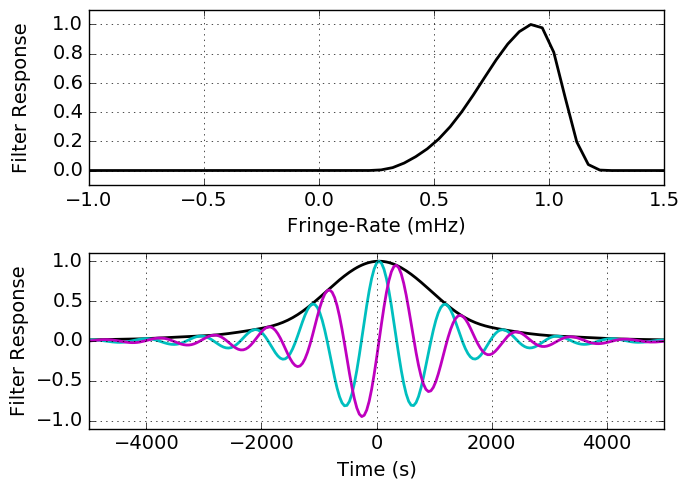
\includegraphics[width=\columnwidth]{plots/frp.png}
	\caption{Top: the normalized optimal power-spectrum sensitivity weighting in fringe-rate space for our fiducial baseline and 
Stokes I polarization beam. Bottom: the time-domain convolution kernel corresponding to the top panel. Real and imaginary 
components are illustrated in cyan and magenta, respectively, with the absolute amplitude in black. The fringe-rate filter acts as 
an integration in time, increasing sensitivity but reducing the number of independent samples in the dataset.}
	\label{fig:frp}
\end{figure}

% SECTION 3 SIGNAL LOSS ---------------------------------------------------------------------------------

\subsection{PAPER-64: Signal Loss}
\label{sec:Sigloss}

In Section \ref{sec:SiglossOverview}, we showed how signal loss arises when weighting data using information from the data 
itself. Here we describe a methodology for estimating the amount of signal loss caused by a particular power spectrum estimator when applied to a particular data set. The exact signal loss ``correction factor" for a particular data set will depend on the specific realizations of the signals present in the data and is not something we can directly compute. 
In this work, we inject simulated cosmological signals into our data and test the recovery of those signals in order to statistically quantify 
the amount of signal loss accompanying a weighting scheme used in OQE power spectrum estimation.  
There are, in fact, several different ways of incorporating the result of such a calculation into a revised power spectrum estimate which accounts for signal loss.  In this section, we describe a methodology for determining an approximate correction factor which can be applied to a power spectrum estimate; in Appendix \ref{sec:Pr_appendix}, we present an alternate framework that explicitly interprets all measurements as upper limits in the presence of signal loss.  
These two methods yield very similar results, but fundamentally are answering subtly distinct questions.  
We also highlight major differences from the signal loss 
computation used in A15, which previously underestimated losses. 

\subsubsection{Signal Loss Methodology} 
\label{sec:siglossmethod}
To capture the full statistical likelihood of signal loss, one requires a quick way to generate many realizations of simulated $21$ 
cm signal visibilities. Here we use the same method as in A15, where mock Gaussian noise visibilities (mock EoR signals) 
are filtered in fringe-rate space to retain only ``sky-like" time-modes. This signal is then added to the data.\footnote{One 
specific change from A15 is that we add this simulated signal into the analysis pipeline before the final fringe-rate filter is 
applied to the data. Previously, the addition was done after that final fringe-rate filter step.  This change results in an increased 
estimate of signal loss, %(by a factor of $\sim$$10$), 
likely due to the use of the fringe-rate filter as a simulator. However, this pipeline difference, while significant, is not the dominant reason why signal loss was under-estimated in A15 (the dominant reason is explained in the main text in Section \ref{sec:Illustration}).}

Suppose that $\textbf{e}$ is a mock injected EoR signal (at some amplitude level), and $\textbf{x}$ is our data. We define $\textbf{r}
$ to be the data plus the EoR signal:

\begin{equation}
\textbf{r} = \textbf{x} + \textbf{e}.
\end{equation}

We are interested in quantifying how much variance in $\textbf{e}$ is lost after weighting $\textbf{r}$ and estimating the power 
spectrum according to OQE formalism. We investigate this by comparing two quantities we call the input power spectrum and 
output power spectrum: $P_{\rm in}$ and $P_{\rm out}$, defined as

\begin{equation}
\label{eq:Pin}
P_{\rm in,\alpha} \equiv M^{\alpha}_{\rm in}\textbf{e}^{\dagger}\textbf{I}\textbf{Q}^{\alpha}\textbf{I}\textbf{e}
\end{equation}

\noindent and

\begin{eqnarray}
\label{eq:sigloss}
P_{\rm out,\alpha} &\equiv& \widehat{\textbf{p}}_{r,\alpha}-\widehat{\textbf{p}}_{x,\alpha} \nonumber \\
&=& M^{\alpha}_{r}\textbf{r}^{\dagger}\textbf{R}_{r}\textbf{Q}^{\alpha}\textbf{R}_{r}\textbf{r} - M^{\alpha}_{x}\textbf{x}^{\dagger}\textbf{R}_{x}\textbf{Q}
^{\alpha}\textbf{R}_{x}\textbf{x},
\end{eqnarray}
where, for illustrative purposes and notational simplicity, we have written these equations with diagonal normalization matrices $M$, even though for our numerical results we choose a non-diagonal matrix $\mathbf{M}$ as in Equation \eqref{eq:phat}. $P_{\rm in}$ represents the unweighted power spectrum of $\textbf{e}$, our simulated EoR signal, 
$\widehat{\textbf{p}}_{x}$ is the power spectrum of the data alone, $\widehat{\textbf{p}}_{r}$ is the power spectrum of the
data plus injection, and $P_{\rm out}$ is the difference between $\widehat{\textbf{p}}_{r}$ and $\widehat{\textbf{p}}_{x}$.

In short, we can approximate a signal loss estimate as the ratio of $P_{\rm out}/P_{\rm in}$, evaluated at the data level $\widehat{\textbf{p}}_{x}$. We motivate the fact that we can evaluate the output-to-input power spectrum ratio at $\widehat{\textbf{p}}_{x}$ by the following reasoning (and then detail our signal loss estimation in practice in the sections that follow).

In the limit of no instrumental noise, the data that we measure, $\x$, is comprised of two signals, such that
\begin{equation}
\x \equiv \f + \s,
\end{equation}
where $\mathbf{f}$ represents the foregrounds and $\mathbf{s}$ represents the cosmological signal. In general, suppose that our power spectrum algorithm passes the data through some function $g$, yielding a lossy estimate of the power spectrum $\phat_{x}$. This can be parametrized as
\begin{equation}
\label{eq:LinearPspecSum}
\langle \phat_{x} \rangle  = \langle g(\x) \rangle = \ell_{\rm fg} \p_{\rm fg} + \ell_{\rm eor} \p_{\rm eor},
\end{equation}
where $\ell_{\rm eor}$ and $\ell_{\rm fg}$ are multiplicative factors accounting for the signal loss in the true EoR 
power spectrum $\p_{\rm eor}$ and true foreground power spectrum $\p_{\rm fg}$, respectively. It is not 
\emph{a priori} obvious why this parameterization is suitable; we thus provide a toy model in Appendix 
\ref{sec:sigloss_appendix} to motivate this, although it should be noted that the derivation is an approximation 
which assumes that the covariance used in the OQE analysis is close to the true covariance with effects due to 
small sample size limited to first order perturbations and thus neglects cross correlation between $x$ and $e$.  
In actual fact the sample size is similar to the number of independent modes, a case were one expects cross 
terms to be remain significant.   

Given this form, a suitable estimate for $\p_{\rm eor}$ would be $\phat_{x} / \ell_{\rm eor}$, or the uncorrected power spectrum of data divided by the signal loss estimate. Although such an estimate leaves an additive bias from foregrounds (see Section \ref{sec:BiasTypes}) that must be mitigated by other methods (as is the case for any attempt to measure the $21\,\textrm{cm}$ power spectrum), it normalizes $\p_{\rm eor}$ back to its correct level such that there is no multiplicative bias. The most conceptually straightforward way to compute $\ell_{\rm eor}$ is to model the foregrounds and EoR signal via simulations, and then to form the quantity
\begin{equation}
\label{eq:Deriv1}
\widehat{\ell}_{\rm eor} = \frac{g(\f + \s) - g(\f)}{\p_{\rm eor}}.
\end{equation}
However, this approach assumes that we have sufficiently good knowledge of our foreground and signal models, which is certainly not the case --- if it were, it would be simpler to construct our covariance matrices from our models, avoiding signal loss altogether! Instead, we can use the data itself as our model of the foregrounds, injecting a new EoR signal $\e$ (with power spectrum $P_{in}$), computing instead
\begin{equation}
\label{eq:Deriv2}
\widehat{\ell}_{\rm eor} = \frac{g(\x+ \e) - g(\x)}{P_{in}},
\end{equation}
which reduces to the same result because of the linearity of Equation \eqref{eq:LinearPspecSum}. Essentially, one is computing the slope of $\langle \phat_{x} \rangle$ with respect to $\p_{\rm eor}$ (note that both Equations \eqref{eq:Deriv1} and \eqref{eq:Deriv2} take the form of finite difference derivatives). Under the approximation that the relation between the two quantities is linear, it does not matter whether this slope is evaluated about $\x$ or $\f$. In reality, one expects some deviations from linearity, but Equation \eqref{eq:Deriv2} remains a good approximation of Equation \eqref{eq:Deriv1} as long as $\x$ is dominated by $\f$. 

Using this motivation, the numerator of Equation \eqref{eq:Deriv2} is precisely our expression for $P_{\rm out}$ (Equation \eqref{eq:sigloss}), and the denominator is $P_{\rm in}$ (Equation \eqref{eq:Pin}), where the function $g$ is our OQE power spectrum pipeline. \dcj{Here is the post-hoc justification for this signal loss method.  Except goes back to assumption of equation for g which just \emph{assumes} that there are no cross terms in the estimation of a power spectrum. So we're just kicking the can down the road.} \acl{Ok, in my defense, Equation \eqref{eq:LinearPspecSum} is a little better than an \emph{assumption}. Appendix \eqref{sec:sigloss_appendix} does in fact illustrate this with an example. The crucial question is whether we're allowed to motivate our method based on a relationship that is only true in expectation. Note that this expectation includes allowances for signal loss due to the cross correlation between signal and foregrounds, with an example of this being Appendix \ref{sec:sigloss_appendix}.}
\jp{I'm fine with leaving the text as is and calling this note closed with the addition of the appendix, but will wait for sign off from DCJ.}
\dcj{ Assuming that expansion to "leading order in $\eta$" means $\eta<<1$ then the approximation is that the 
covariance is nearly perfectly calculated from the data with only small effects due to finite samples. Thus 
correlations don't make it into the expression and foregrounds remain uncorrelated with eor or injected signals.  
I added words explaining this but it still looks strange for us to be saying that loss is linear in one section and 
then explaining in the next section exactly how cross terms were what messed us up in the first go round.} 
\acl{Ok, I'm open to suggestions as to how to phrase this, because lots of people seem to be thinking that the appendix was meant to justify everything. It's not. It's meant as a motivational example. I just wanted something where I could follow through analytically to the end to show that it's ok to think about signal loss as a multiplicative factor. At least in expectation. And then how one deals with not correcting for the signal loss in expectation is described in Section \ref{sec:Practice}.}

Effectively, this means that the relationship between the input and output power spectra, $P_{\rm in}$ and $P_{\rm out}$, can be thought of as a transfer function 
which, for a sampling of $P_{\rm in}$ and $P_{\rm out}$ provides a mapping from an input power spectrum distribution into an output 
distribution. By viewing data through this signal loss lens, we may then ask the question ``what input power spectrum 
distribution could this (signal-loss affected) data come from?" 

In Section \ref{sec:Illustration}, we provide some intuition for how the transfer function is able to capture signal loss. Section \ref{sec:Practice} then details the numerical computations used to translate our power spectrum result into one viewed through a 
signal loss lens. We note that interpretation of the signal injection results can be framed in multiple ways which yield similar but not identical answers. One alternative to the method described in Section \ref{sec:Practice} is described in Appendix \ref{sec:Pr_appendix}.
%We showcase two methods... \cc{fill in with some broad statement of why we're showing 2 methods but also state that they yield similar results...}

\subsubsection{Signal Loss Illustration}
\label{sec:Illustration}
To explore how our expression for $P_{\rm out}$ encapsulates signal loss, we expand out Equation \eqref{eq:sigloss}:

\begin{eqnarray}
\label{eq:crossterm}
P_{\rm out,\alpha} &=& M^{\alpha}_{r}(\textbf{x}+\textbf{e})^{\dagger}\textbf{R}_{r}\textbf{Q}^{\alpha}\textbf{R}_{r}(\textbf{x}+\textbf{e}) - 
M^{\alpha}_{x}\textbf{x}^{\dagger}\textbf{R}_{x}\textbf{Q}^{\alpha}\textbf{R}_{x}\textbf{x} \nonumber \\
&=& M^{\alpha}_{a}\textbf{x}^{\dagger}\textbf{R}_{r}\textbf{Q}^{\alpha}\textbf{R}_{r}\textbf{x} + M^{\alpha}_{b}\textbf{e}^{\dagger}\textbf{R}_{r}\textbf{Q}
^{\alpha}\textbf{R}_{r}\textbf{e} \nonumber \\
&+& M^{\alpha}_{c}\textbf{x}^{\dagger}\textbf{R}_{r}\textbf{Q}^{\alpha}\textbf{R}_{r}\textbf{e} + M^{\alpha}_{d}\textbf{e}^{\dagger}\textbf{R}_{r}\textbf{Q}^{\alpha}\textbf{R}_{r}\textbf{x} \nonumber \\
&-& M^{\alpha}_{x}\textbf{x}^{\dagger}\textbf{R}_{x}\textbf{Q}
^{\alpha}\textbf{R}_{x}\textbf{x}.
\end{eqnarray}
We see that $P_{\rm out}$ is comprised of multiple terms. To build intuition into each of these terms, they are plotted individually in Figure \ref{fig:sigloss_terms} for two cases: inverse covariance weighting ($\textbf{R}_{r} = \widehat{\textbf{C}}_{r}^{-1}$, left) and unweighted ($\textbf{R}_{r} = \textbf{I}$, right). We leave the details of the simulation to Section \ref{sec:Practice}, but for now highlight that each term in Equation \eqref{eq:crossterm} corresponds to a different color in the plot. Specifically, the first term in Equation \eqref{eq:crossterm} is plotted as blue, the second as green, the third and fourth (which are the same) as red, and the last as gray. The solid black curve denotes $P_{\rm out}$, which is comprised of all the other terms.

A brief description of Figure \ref{fig:sigloss_terms} is as follows. The gray curve represents the data level, which is constant as the level of $P_{\rm in}$, the input EoR signal, is changed. The blue curve is the power spectrum of the data only, weighted by an empirical covariance estimated from the data plus the EoR signal ($\widehat{\textbf{C}}_{r}^{-1}$). It approaches the gray at low injection level, as expected, since in that case $\widehat{\textbf{C}}_{r}^{-1} \rightarrow \widehat{\textbf{C}}_{x}^{-1}$. The green curve is the power spectrum of the EoR signal, weighted by $\widehat{\textbf{C}}_{r}^{-1}$. This is the exact term that was compared to $P_{\rm in}$ in the A15 signal loss analysis, and in doing so this would imply there is negligible loss (where the green crosses the gray). It is primarily due to the cross-terms (red), that the black curve exhibits $\sim$$3$ orders of magnitude of loss at the data level, for the inverse covariance weighted case. We see that the cross-terms can produce a large, negative signal which serves to reduce $P_{\rm out}$ and drive the bulk of our loss. In the unweighted case, however (right plot), the cross-terms primarily drive a tail of `excess' $P_{\rm out}$ at low injects, though at larger injects we see unity transfer as expected (the solid black curve lies on the dotted black line, which represents unity transfer).

We now turn to building intuition behind the negative power that arises from the cross-terms in Equation \eqref{eq:crossterm}. For illustrative purposes in this subsection only, we consider a scenario where $\textbf{e}$ dominates compared to $\textbf{x}$. It is in this limit where we expect signal loss to be greatest, and $P_{\rm out}$ becomes:

\begin{eqnarray}
\label{eq:pout_expand}
P_{\rm out, \alpha} &\approx&  M^{\alpha}_{b}\textbf{e}^{\dagger}\textbf{R}_{r}\textbf{Q}^{\alpha}\textbf{R}_{r}\textbf{e} +
 2M^{\alpha}_{c}\textbf{x}^{\dagger}\textbf{R}_{r}\textbf{Q}^{\alpha}\textbf{R}_{r}\textbf{e}.
\end{eqnarray}
The first term of $P_{\rm out}$ is simply the weighted power spectrum of $\textbf{e}$ alone. Again, it is this quantity that was used in A15 to calculate signal loss. However, without taking into account the cross-terms (the second term), we can substantially under-estimate loss. In short, this is because correlations between the data and injected EoR signal emerge as statistical noise that is added to the power spectrum estimate, decreasing the value of $P_{\rm out}$. Including these cross-terms in our new analysis represents the bulk change of our revised analysis compared to A15.

\begin{figure*}
	\centering
	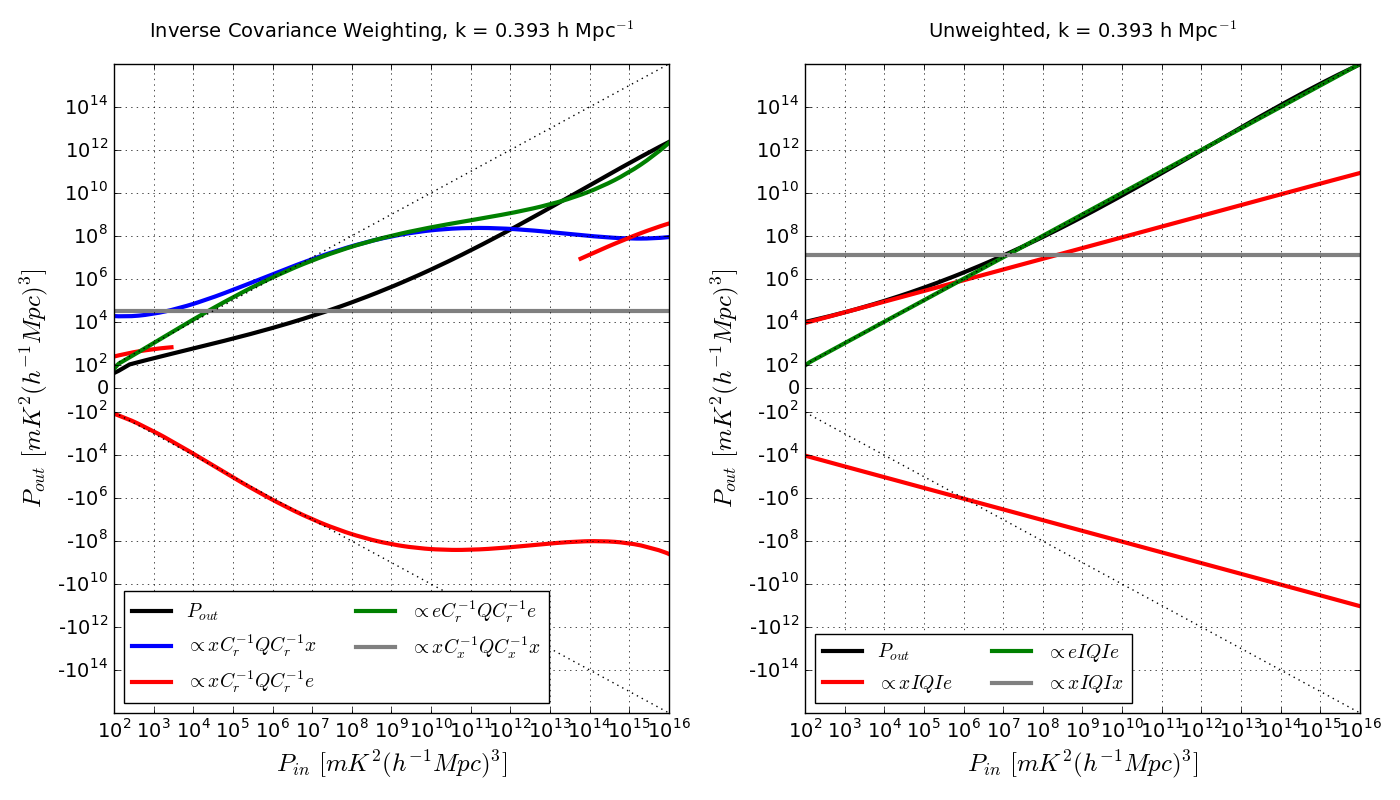
\includegraphics[width=1\textwidth]{plots/sigloss_terms.png}
	\caption{Illustration of the components of the signal loss transfer function, $P_{\rm out}$, as defined by Equation \eqref{eq:crossterm} for PAPER-64 data for the inverse covariance weighted case (left) and unweighted case (right). The details of the simulation used to generate the figure is explained in Section \ref{sec:Practice}; here we fit smooth polynomials to our data points to create the curves. We show the contributions of each signal loss term (blue, red, green, gray), which when combined produce the black $P_{\rm out}$ curve. Most notably, the green curves denotes the signal loss analysis used in A15, and the red curves showcase the importance of the cross-terms in Equation \eqref{eq:crossterm} in computing signal loss. As explained in the main text, the cross-terms can produce large, negative signal which represents the difference between the green curve (which exhibits negligible loss at the data level) and the black curve (which exhibits $\sim$$3$ orders of magnitude of loss at the data level for the inverse covariance weighted case). Finally, the dotted diagonal black line represents perfect unity transfer, or no signal loss, which we recover for the unweighted case.}
	\label{fig:sigloss_terms}
\end{figure*}

When $\textbf{R}_{r}$
is taken to be $\widehat{\textbf{C}}_{r}^{-1}$, the second term of Equation \eqref{eq:pout_expand} is a cross-correlation between $\widehat{\textbf{C}}_{r}^{-1}\textbf{x}$ and
$\widehat{\textbf{C}}_{r}^{-1}\textbf{e}$. As shown in \citet{switzer_et_al2015}, this cross-correlation term is non-zero, and in fact negative in expectation. 
This negative cross-term power arises from a coupling between the inverse of 
$\widehat{\textbf{C}}_{r}$ and $\mathbf{x}$. 
Intuitively, we can see this by expanding the empirical covariance of $\textbf{r}=\textbf{x}+\textbf{e}$ in the
$|\textbf{x}|\ll|\textbf{e}|$ regime:

\begin{eqnarray}
\widehat{\textbf{C}}_{r} &=& \langle \textbf{rr}^{\dagger} \rangle_{t} \nonumber \\ 
&=& \langle \textbf{xx}^{\dagger} \rangle_{t} + \langle \textbf{xe}^{\dagger} \rangle_{t} + \langle \textbf{ex}^{\dagger} \rangle_{t} + \langle 
\textbf{ee}^{\dagger} \rangle_{t},
\end{eqnarray}

\noindent where we can neglect the first term because $\textbf{x}$ is small.  Without loss of generality, we will assume
an eigenbasis of $\textbf{e}$, so that $\langle 
\textbf{ee}^{\dagger} \rangle_{t}$ is diagonal. 
The middle 
two terms, however, can have power in their off-diagonal terms due to the fact that, when averaging over a finite
ensemble, $\langle\textbf{xe}^\dagger\rangle_t$ is not zero.  As shown in Appendix C of \citet{parsons_et_al2014}, to leading order the
inversion of a matrix like $\widehat{\textbf{C}}_{r}$ that is diagonal-dominant (from $\langle 
\textbf{ee}^{\dagger} \rangle_{t}$) with smaller
off-diagonal terms results in a new diagonal-dominant matrix with negative off-diagonal terms. These off-diagonal
terms depend on both $\textbf{x}$ and $\textbf{e}$. When $\widehat{\textbf{C}}^{-1}_{r}$ is multiplied into $\textbf{x}$,
the result is a vector that is similar to $\textbf{x}$ but
contains a residual correlation to $\textbf{e}$ from the off-diagonal components of $\widehat{\textbf{C}}^{-1}_{r}$. The
correlation is negative because the product $\widehat{\textbf{C}}_r^{-1}\textbf{x}$ effectively squares the $\textbf{x}$-dependence
of the off-diagonal terms in $\widehat{\textbf{C}}^{-1}_{r}$ while retaining the negative sign that arose from the inversion
of a diagonal-dominant matrix.
% XXX [ARP: we may want to write this all out explicitly in an appendix]

The correlation between $\widehat{\textbf{C}}_r^{-1}\textbf{e}$ and $\widehat{\textbf{C}}_r^{-1}\textbf{x}$ means that we cannot compute signal loss using a signal-only 
simulation, which would yield greater values for $P_{\rm out}$ and thereby underestimate signal loss. Therefore, in our revised 
signal loss computation we use the full quantity for $P_{\rm out}$ as defined in Equation \eqref{eq:sigloss}, which subtracts the 
weighted power spectrum of the data from the weighted power spectrum of data plus EoR. 

We thus see from this subsection that signal loss generically arises because of couplings between $\widehat{\textbf{C}}^{-1}_{r}$ and $\mathbf{x}$. In principle, using $\widehat{\textbf{C}}^{-1}_{r}$ in place of the true inverse covariance $\textbf{C}^{-1}$ provides yet another source of multiplicative bias, which results in a modification to the treatment shown here. Such a modification is accounted for in the demonstration of Appendix \ref{sec:sigloss_appendix}, where we additionally discard the assumption that $|\textbf{x}|\ll|\textbf{e}|$. However, despite the loosening of these approximations, one sees that the qualitative message (of anti-correlations resulting in signal loss) remains intact.



\subsubsection{Signal Loss in Practice}
\label{sec:Practice}
%\begin{center}
%METHOD \#1
%\end{center}

We now shift our attention towards computing signal loss for the fringe-rate filtered PAPER-64 dataset. While our methodology 
outlined below is independent of weighting scheme, here we demonstrate the computation using inverse covariance weighting 
($\textbf{R} = \widehat{\textbf{C}}^{-1}$), the weighting scheme used in A15 which, with an empirically estimated covariance, leads to substantial loss. With this weighting, our 
expressions for $P_{\rm in}$ and $P_{\rm out}$ become

\begin{eqnarray}
P_{\rm in,\alpha} &=&  M^{\alpha}_{\rm in}\textbf{e}^{\dagger}\textbf{I}\textbf{Q}^{\alpha}\textbf{I}\textbf{e} \\
P_{\rm out,\alpha} &=&  M^{\alpha}_{r}\textbf{r}^{\dagger}\widehat{\textbf{C}}_{r}^{-1}\textbf{Q}^{\alpha}\widehat{\textbf{C}}_{r}^{-1}\textbf{r} \nonumber \\
&&\phantom{=====} 
-  M^{\alpha}_{x}\textbf{x}^{\dagger}\widehat{\textbf{C}}_{x}^{-1}\textbf{Q}^{\alpha}\widehat{\textbf{C}}_{x}^{-1}\textbf{x}. 
\end{eqnarray}

The treatment we outlined in the previous section implicitly assumed that signal loss corrections could be treated in expectation. In practice, however, the signal loss itself is a random variable --- some realizations of the cosmological signal may be more correlated with foreground modes than others, leading to more signal loss. This leads to two issues. The first is that Equation \eqref{eq:LinearPspecSum} may not hold. In particular, a third term that is a quadratic combination of $\f$ and $\s$ (e.g., $\f^\dagger \C^{-1} \s$) may appear. However, we can circumvent this issue by decomposing $\f$ into a sum of two vectors, one that is proportional to $\s$ and one that is orthogonal to $\s$. The former can be absorbed into the EoR term (part of the signal loss estimate), while the latter can be absorbed into the foreground term. In other words, suppose that we have
\begin{equation}
\phat_x \approx \ell_{\rm fg} |\mathbf{f}|^2 + \ell_{\rm eor} |\mathbf{e}|^2 + \ell_{\rm fe} \mathbf{f} \cdot \mathbf{e}.
\end{equation}
in place of Equation \eqref{eq:LinearPspecSum}. Now, split $\mathbf{f}$ into $\mathbf{ f}_\parallel +\mathbf{ f}_\perp$, which are the components of the foregrounds that couple to the EoR versus those that do not. Further parameterize $\mathbf{ f}_\parallel \equiv \rho \mathbf{e}$, where $\rho$ is some correlation coefficient that quantifies the degree of correlation between the foregrounds and the EoR. This then gives
\begin{equation}
\label{eq:fperpfpara}
\phat_x \approx \ell_{\rm fg} |\mathbf{f}|^2 +( \ell_{\rm eor} + \rho  \ell_{\rm fe} ) |\mathbf{e}|^2 + \ell_{\rm fe} \mathbf{f}\cdot \mathbf{f}_\perp.
\end{equation}
Since $|\mathbf{e}|^2$ would be a lossless estimate of the true EoR power spectrum, this expression recovers the linear relation between the true EoR power spectrum and the lossy estimate.
\dcj{Wait what? I think you are saying essentially that some x can remain in Pout which is what we are seeing. Or is this some extra bit of method which has been added to the analysis...} \acl{I'm not sure that's what I'm saying. (And by ``I'm not sure" I don't mean it in the colloquial sense of ``you're not right and I'm just trying to be polite about it", but rather the literal sense of the phrase ``I'm not sure"). What I was trying to say was that if I wrote Equation \eqref{eq:LinearPspecSum} without the ensemble average, I could say
\begin{equation}
\phat_x \approx \ell_{\rm fg} f^2 + \ell_{\rm eor} e^2 + \ell_{\rm fe} fe.
\end{equation}
(Note that even this is an approximation. In principle there is an infinite series containing all possible powers of 
$e$ and $f$). Now, we split $f$ into $ f_\parallel + f_\perp$, which are the components of the foregrounds that 
couple to the EoR versus those that do not. Further parameterize $f_\parallel \equiv \rho e$, where $\rho$ is 
some correlation coefficient that quantifies the degree of correlation between the foregrounds and the EoR. 
Under this parameterization, one can write the $fe$ term in terms of $e^2$ (which gets absorbed into the other 
EoR term, plus residual foregrounds that we don't care about).}\acl{Just promoted this last part to something in 
the main text.}\dcj{I will admit to being a little lost here.  Doesn't changing the basis just convert the unknown f 
dot s term into other unknown terms. Isn't the whole point of Eq 24 supposed to be that we can subtract off the 
$g(x)$ to estimate $\hat{\ell}_{\rm eor}$?  How do we subtract off $f\dot f_\perp$? Don't we want to know $
\ell_{\rm eor}$ not $(\ell_{\rm eor} + \rho\ell_{\rm fe})$? }
\acl{I think what we are trying to say here is that actually the thing we want \emph{is} $(\ell_{\rm eor} + \rho\ell_{\rm fe})$. Essentially, the potential coupling between the injected EoR and the foregrounds means that we lose the nice form of Equation \eqref{eq:LinearPspecSum}, which justified what is basically a multiplicative correction to signal loss. What we are suggesting here is that even when there is a coupling, the estimator can be parameterized as $\alpha  |\mathbf{e}|^2 + \beta$. So essentially we are defining an effective $
\ell_{\rm eor}$, which is given by $(\ell_{\rm eor} + \rho\ell_{\rm fe})$.}

The second issue to tackle is how one incorporates the randomness of $\ell_{\rm eor}$ into our signal loss corrections. This is manifest in Equation \eqref{eq:fperpfpara}, where the randomness of $\rho$ means that there is an inherent spread in the signal loss correction. Phrased in the context of Bayes' rule, we wish to find the posterior probability distribution of $p( \p_{\rm eor} | \phat_{x})$ for $\p_{\rm eor}$ given the uncorrected power spectrum estimate $\phat_{x}$. Since Equation \eqref{eq:Deriv2} is a good approximation of Equation \eqref{eq:Deriv1}, which we argued for in the previous section, we can write $\p_{\rm eor}$ as $P_{in}$, and hence the probability distribution is given by
\begin{equation}
\label{eq:Bayes}
p(P_{in} | \phat_{x}) \propto \mathcal{L} (  \phat_{x} | P_{in})  p(P_{in}),
\end{equation}
where $p(P_{in})$ is the prior on $P_{in}$ and $\mathcal{L} $ is the likelihood function. Since the likelihood is defined as the distribution of the measured result $ \phat_{x}$ given the theoretical power spectrum $P_{in}$, we may construct this function simply by fixing $P_{in}$, and simulating our analysis pipeline for many realizations of the injected EoR signal consistent with this power spectrum. The resulting distribution can be normalized, and the whole process can then be repeated for a different value of $P_{in}$. 

In our code, we simulate $20$ realizations of $P_{in}$, yielding $P_{\rm in}$ values that range from $\sim$$10^{2}$ mK$^{2}$ (h$^{-1}$ Mpc)$^{3}$ to $\sim$10$^{16}$ mK$^{2}$ (h$^{-1}$ Mpc)$^{3}$. We also run $25$ total EoR injection levels, resulting in a total of $500$ data points on our $P_{\rm in}$ vs. $P_{\rm out}$ grid. 
%Additionally, we have verified that the transfer function is symmetric for negative and positive $P_{\rm in}$'s, and so we fold all the values into positive ones to increase our signal-to-noise.

We smooth the 2D distribution of $P_{in}$ vs. $P_{out}$ using kernel density estimators. The result, for inverse covariance weighting, is shown in the left plot of Figure \ref{fig:sigloss_transfercurve}. Bayes' rule then simply instructs us to fix $\phat_{x}$ at our measured value, essentially reading Figure \ref{fig:sigloss_transfercurve} horizontally and reinterpreting Equation \eqref{eq:Bayes} as a function of $p(P_{in})$. The final result can then be normalized to give $p(P_{in} | \phat_{x})$. If $\phat_{x}$ itself does not take on a single value but is itself a distribution (for our analysis, this comes from bootstrapping), then one simply repeats the process for every single point on the distribution of $\phat_{x}$, before performing the final summation and normalization. In Figure \ref{fig:sigloss_transfercurve}, the peak of our data distribution $
\widehat{\textbf{p}}_{x}$ is marked by the solid gray horizontal lines. From the left plot (inverse covariance weighting), one can eyeball that a data value of $10^{5} \, mK^{2} (h^{-1} Mpc)^{3}$, for example, would map approximately to a 
value of $\sim10^{8} \, mK^{2} (h^{-1} Mpc)^{3}$, implying a signal loss factor of $\sim1000$. Performing a summation and normalization for the entire distribution of $\widehat{\textbf{p}}_{x}$ yields a final $P_{\rm in}$ distribution --- the distribution of our data as seen through the signal loss lens. We compute power spectrum points from the peak of the histograms, and power spectrum errors from $95\%$ confidence intervals.

As a final complication to our procedure, we note that there will be some intrinsic scatter in our likelihood due to our having only a finite number of simulations. Ideally, running many simulations would lead to convergence in our likelihood; however, our desire to be able to quickly and easily estimate signal loss for a variety of weighting schemes and datasets means having a finite sample in practice. To separate the intrinsic stochasticity of signal loss from that which arises due to simulation noise, we repeat our analysis for a power spectrum estimator without signal loss ($\textbf{R} = \textbf{I}$), shown as the right plot in Figure \ref{fig:sigloss_transfercurve}. This intrinsic scatter is shown as the smeared `heat-map' around the solid black diagonal line (representing unity-transfer) in the plot. The width of the lossless scenario's signal loss likelihood is then deconvolved from the lossy scenario's signal loss likelihood. Specifically, we deconvolve Gaussian distributions of $P_{out}$ in the unweighted case from those of the weighted case (vertical cuts through the plots in Figure \ref{fig:sigloss_transfercurve}), for every $P_{in}$. By doing this, we are left with only the intrinsic scatter in signal loss, or scatter that stems from how much the random EoR signal $\textbf{e}$ happens to 
look like the data $\textbf{x}$, a quantity we do not know offhand but one that we would like to correct for. As an extreme example, if we are very unlucky, one realization of $\textbf{e}$ would have the same shapes, or eigenvectors, as $\textbf{x}$. An empirically-derived covariance would then down-weight these shapes, destroying the entire EoR signal. On the other hand, the less that $\textbf{e}$ looks like $\textbf{x}$, the less signal loss that would result. The intrinsic scatter we can get is not a dominant factor in this case but it is important to correct for the fact that a particular $P_{\rm out}$ value could arise from a range of $P_{\rm in}$ values. 

%The solid black diagonal line in Figure \ref{fig:sigloss_transfercurve} shows unity-transfer, which we expect to occur for the 
%nweighted case ($\textbf{R} = \textbf{I}$). Therefore, it is worth thinking about the spread, or scatter, around this black line that 
%we see in the right plot (the colored `heat-map'). One might imagine that there should be one true $P_{\rm out}$ value for every 
%$P_{\rm in}$, implying one well-determined signal loss factor for every data value. Focusing on the unweighted case alone, the 
%scatter observed arises from the fact that the values of the cross-terms involving $\textbf{e}$ and $\textbf{x}$ in Equation 
%\eqref{eq:pout_expand} change for different mock EoR signals, $\textbf{e}$. Since we draw different random $\textbf{e}$'s for 
%every bootstrap (for reasons made clear in the next paragraph), there is a range of $P_{\rm out}$ values that results from the same 
%$P_{\rm in}$. This randomness causes the spread seen in the right plot of Figure \ref{fig:sigloss_transfercurve}, as well as most of 
%the spread in the weighted case (left plot).

\begin{figure*}
	\centering
	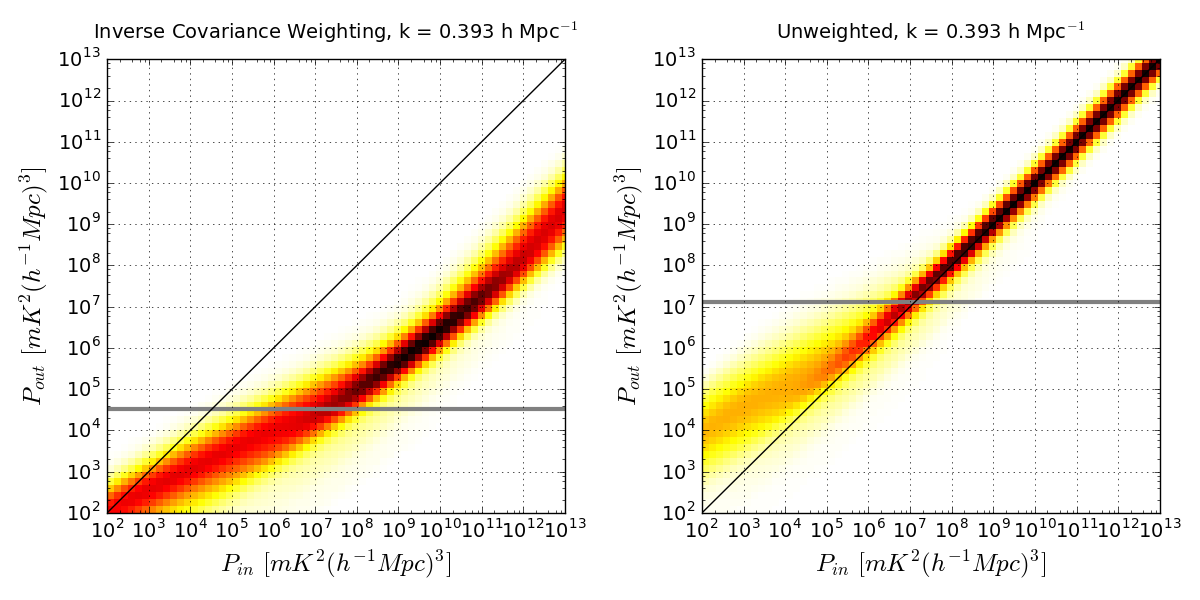
\includegraphics[width=1\textwidth]{plots/sigloss_transfercurve.png}
	\caption{Signal loss transfer functions showing the relationship of $P_{\rm in}$ and $P_{\rm out}$, as defined by Equations \eqref{eq:Pin} and \eqref{eq:sigloss}. Kernel density estimations of the power spectrum transfer functions are shown as colored 
heat-maps for the cases of inverse covariance weighted PAPER-64 data (left) and unweighted data (right). The solid black 
diagonal line marks a perfect unity mapping, and the solid gray horizontal line denotes the power spectrum value of the data $\widehat{\textbf{p}}_{x}$. From these plots, it is clear that inverse covariance weighting results in $\sim3$ orders of magnitude of signal loss 
for power spectrum values above $\sim$$2 \times 10^{4}$ $mK^{2} \, (h^{-1} \, Mpc)^{3}$, whereas the unweighted case does 
not exhibit loss. The peculiar `signal gain' tail seen at low injection is driven by the cross-terms in Equation \eqref{eq:pout_expand}, also shown by the red curve in the right panel in Figure \ref{fig:sigloss_terms}.}
	\label{fig:sigloss_transfercurve}
\end{figure*}

%One peculiar aspect of Figure \ref{fig:sigloss_transfercurve} is the fact that at low $P_{\rm in}$ values it appears that we can have signal gain ($P_{\rm out} > P_{in}$). \cc{This is a log-plotting effect and is under-construction!}.
%This is unphysical in nature but caused due to the dominating cross-terms involving $\textbf{e}$ and $\textbf{x}$ in Equation \eqref{eq:pout_expand} once $\textbf{e}$ becomes small. 

The shape of our signal loss transfer function can be described as follows. At low injection levels, for small $\textbf{e}$, we are dominated by the cross-terms involving $\textbf{e}$ and $\textbf{x}$ in Equation \eqref{eq:pout_expand}. As $\textbf{e}$ increases, we move 
into a regime where $P_{\rm out} \sim P_{in}$, and then eventually into a regime where $P_{\rm out} < P_{in}$ when $\textbf{e}$ is 
large enough to be destroyed if weighting the data using itself. Although we only show figures for one $k$ value, we note that 
the shape of the transfer curve is nearly identical for all $k$'s (though we treat each $k$ separately).

%\begin{figure*}
%	\centering
%	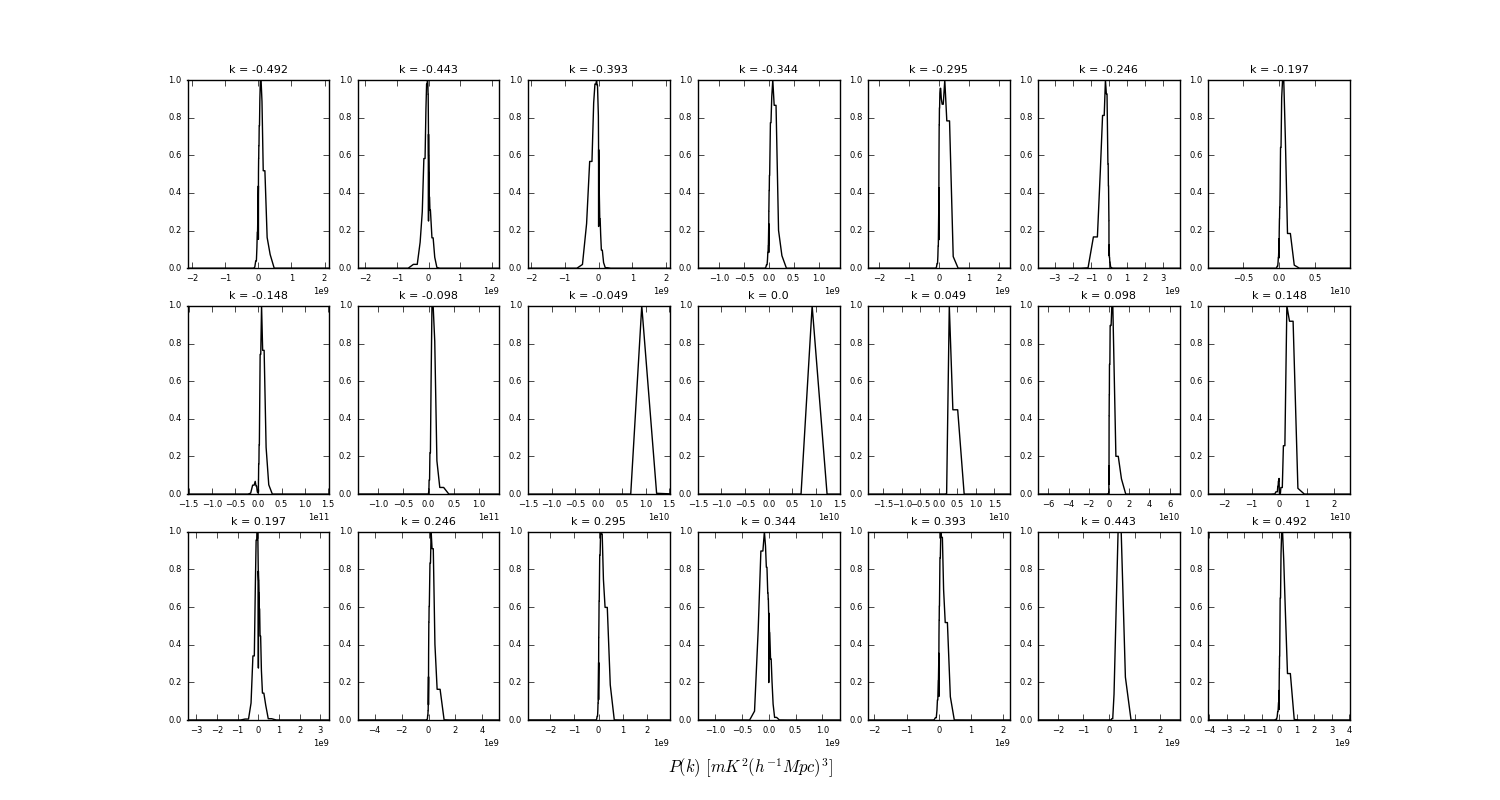
\includegraphics[trim={1cm 0cm 1cm 1cm},width=1\textwidth]{plots/sigloss_datadist_inversecovariance.png}
%	\caption{Normalized histograms of the power spectra that result from using inverse covariance weighting on %PAPER-64 data after signal loss correction. Power spectrum points are computed from the peak of the distributions. Errors are computed using $95\%$ confidence intervals.}
%	\label{fig:sigloss_datadist_inversecovariance}
%\end{figure*}

To conclude this method, we also show power spectrum results for fringe-rate filtered PAPER-64 data before and after signal 
loss estimation in Figure \ref{fig:ps2_data}, using empirically estimated inverse covariance weighting. The blue dashed line represents the unweighted 
power spectrum $2\sigma$ upper limit, which is identical in both panels (an important check, as we expect no signal loss for this case). The black and 
gray points are positive and negative power spectrum values plotted with $2\sigma$ error bars. Prior to signal loss estimation, it 
is clear that the power spectrum is unfeasible because it is well below the theoretical noise level prediction (solid green curve). 
Post-estimation, the power spectrum errors are higher than both the theory and unweighted power spectrum, a consequence of weighting with a steep eigenspectrum where the `weak' modes are strongly coupled to the time-averaged fringe-rate filtered data. We elaborate on this point in the next section, as well as investigate alternate 
weighting schemes to inverse covariance weighting, with the goal of finding one that balances the aggressiveness of down-weighting contaminants with minimizing the loss of EoR signal. 

\begin{figure*}
	\centering
	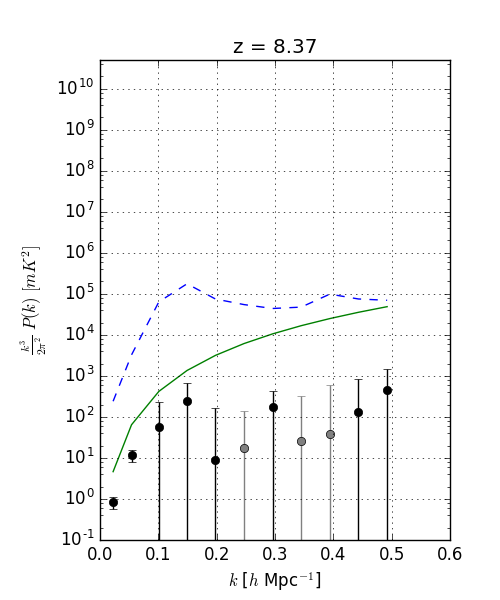
\includegraphics[width=0.4\textwidth]{plots/ps2_data_nosigloss.png}
	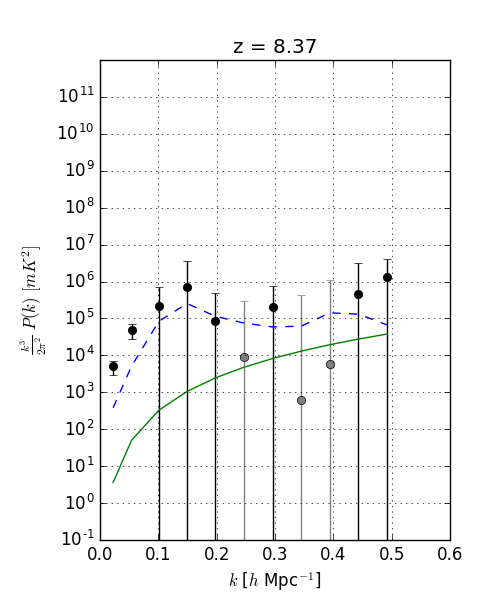
\includegraphics[width=0.4\textwidth]{plots/ps2_data.png}
	\caption{Full inverse covariance weighted power spectrum of PAPER-64 data (positive points in black and negative points in gray, 
with $2\sigma$ error bars) before signal loss estimation (left) and after (right). The dashed blue line is the unweighted power 
spectrum ($2\sigma$ upper limit). The solid green line is the theoretical $2\sigma$ noise level prediction based on observational 
parameters, whose calculation is detailed in Section \ref{sec:PSSense}.}
	\label{fig:ps2_data}
\end{figure*}


\subsubsection{Minimizing Signal Loss}
\label{sec:Weight}

With a signal loss formalism established, we now have the capability of experimenting 
with different weighting options for $\textbf{R}$. Our goal here is to choose a weighting method that successfully down-weights 
foregrounds and systematics in our data without generating large amounts of signal loss. We have found that the balance 
between the two is a delicate one and requires a careful understanding and altering of empirical covariances. 

We saw in Section \ref{sec:otherweight} how limiting the number of down-weighted eigenmodes (i.e. flattening out part of the 
eigenspectrum and effectively de-coupling the `weak' eigenmodes from the data) can help minimize signal loss. We experiment with this idea on PAPER-64 data, dialing the number of modes 
that are down-weighted from zero (which is equivalent to identity-weighting, or the unweighted case) to $21$ (which is full inverse 
covariance weighting of our $21$ channels). The power spectrum results for one $k$ value, both before and after signal loss 
estimation, are shown in the top panel in Figure \ref{fig:sigloss_modeloop}. We see that the amount of signal loss increases as weighting 
becomes more aggressive (gray curve). In other words, more `weak' (EoR-dominated) fluctuations are being overfit and 
subtracted as more modes are down-weighted. We also find that the power spectrum upper limit, post signal loss estimation, 
increases with the number of down-weighted modes (black curve). The more modes we use in down-weighting, the stronger the coupling between the weighting and the data, and the greater the error we have in estimating the power spectrum.

Optimistically, we expect there to be a `sweet spot' as we dial our regularization knob; a level of regularization where weighting 
is beneficial compared to not weighting (blue dashed line). In other words, we would like a weighting scheme that down-weights eigenmodes that predominantly describe foreground modes, but not EoR modes. We see in Figure \ref{fig:sigloss_modeloop} that this occurs when 
only the strongest $\sim3$-$4$ eigenmodes are down-weighted, though the improvement from the unweighted case is small. 

We also saw in Section \ref{sec:otherweight} how adding the identity matrix to the empirical covariance can minimize signal loss. We experiment with this idea as well, shown in the bottom panel of Figure \ref{fig:sigloss_modeloop}. The grey and black lines represent power spectrum limits pre and post signal loss estimation, respectively, as a function of the strength of $\textbf{I}$ that is added to $\widehat{\textbf{C}}$, quantified as the percentage of the $Tr(\widehat{\textbf{C}})$ added to $\widehat{\textbf{C}}$. When $0\%$  of the $Tr(\widehat{\textbf{C}})$ is used, it is equivalent to full inverse covariance weighting. From this plot we see that only a small percentage of $Tr(\widehat{\textbf{C}})$ is needed to significantly reduce loss. We expect that as the strength of $\textbf{I}$ is increased (going to the left), both the black and gray curves will approach the unweighted case.

\begin{figure*}
	\centering
	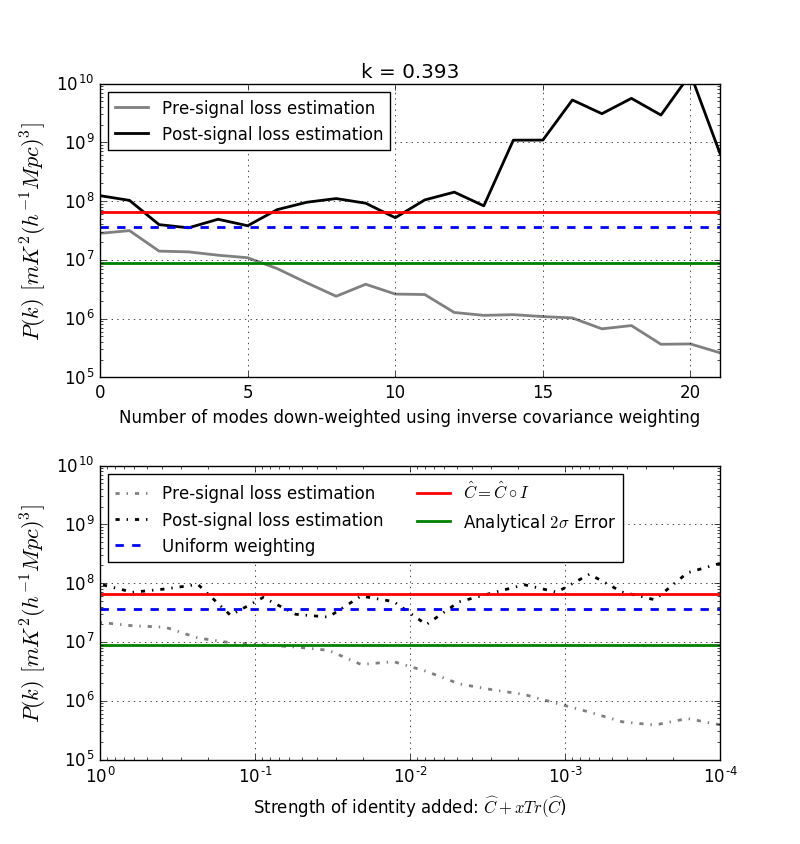
\includegraphics[width=1\textwidth]{plots/sigloss_modeloop_2panel.png}
	\caption{Power spectra $2\sigma$ upper limits for $k=0.393$ h Mpc$^{-1}$ for fringe-rate filtered PAPER-64 data. Top: Values 
are shown before (gray) and after (black) signal loss estimation as a function of number of eigenmodes of $\widehat{\textbf{C}}$ that 
are down-weighted. This regularization knob is tuned from $0$ modes on the left (i.e. unweighted) to $21$ modes on the right (i.e. full inverse 
covariance weighting). Over $\sim3$ orders of magnitude of signal loss results when using inverse covariance weighting. Bottom: Power spectrum upper limits before (gray) and after (black) signal loss estimation as a function of identity added to the empirical covariance. This regularization knob is tuned from $0\%$  of the $Tr(\widehat{\textbf{C}})$ added to $\widehat{\textbf{C}}$ on the right (i.e. full inverse covariance weighting) to $20\%$ of $Tr(\widehat{\textbf{C}})$ added to $\widehat{\textbf{C}}$ on the left. Also 
plotted in both panels for comparison are $2\sigma$ power spectrum upper limits for the unweighted case (dashed blue) and inverse variance 
weighted case (red); both are after signal loss estimation. Finally, a theoretical prediction for noise ($2\sigma$ error) is plotted 
as solid green. In the revised PAPER-64 analysis in this paper, we choose to use a regularization scheme of $\widehat{\textbf{C}} \equiv 0.04Tr(\widehat{\textbf{C}}) + \widehat{\textbf{C}}$ because it outperforms both the down-weighting individual eigenmodes and inverse variance cases.}
	\label{fig:sigloss_modeloop}
\end{figure*}

In addition to our thermal noise prediction (green) and unweighted power spectrum limit (blue), one additional horizontal line is shown in Figure \ref{fig:sigloss_modeloop} 
in both panels and represents a third regularization technique. This line (red) denotes the power spectrum value, post-signal loss estimation, for inverse variance weighting (multiplying an identity 
matrix element-wise to $\widehat{\textbf{C}}$). This result is single-valued and not a function of the x-axes. We see that all three regularization schemes shown (black solid, black dashed, red) perform similarly at 
their best (i.e. when $\sim3$$-4$ eigenmodes are down-weighted in the case of the black solid curve). However, for the remainder of this paper, we choose to use the weighting option of $\widehat{\textbf{C}} \equiv \widehat{\textbf{C}} + 0.04Tr(\widehat{\textbf{C}})$, which we will denote as $\widehat{\textbf{C}}_{eff}$. We choose this weighting scheme because it slightly out-performs the other weighting schemes, likely due to the fact that it retains information from all eigenmodes (i.e. it doesn't throw away some information as in the other cases) but re-weights them in a way that produces minimal loss.

Our revised, best to-date PAPER-64 power spectrum (using only one baseline separation type and $\widehat{\textbf{C}}_{eff}$) is shown in Figure 
\ref{fig:ps1_data}. Again, black and gray points correspond to positive and negative power spectrum values respectively, with 
$2\sigma$ errors bars. Also plotted are the unweighted power spectrum upper limit (dashed blue) and theoretical prediction of 
noise (solid green). From this result, we quote a best $2\sigma$ upper limit of $(151.0$ mK$)^{2}$ at $k=0.34$ $h$Mpc$^{-1}$, 
a higher limit than A15 by a factor of $\sim7$ in mK (though we only use one baseline type in our analysis as opposed to three). 
\cc{replace with kolopanis limit instead later}

\begin{figure*}
	\centering
	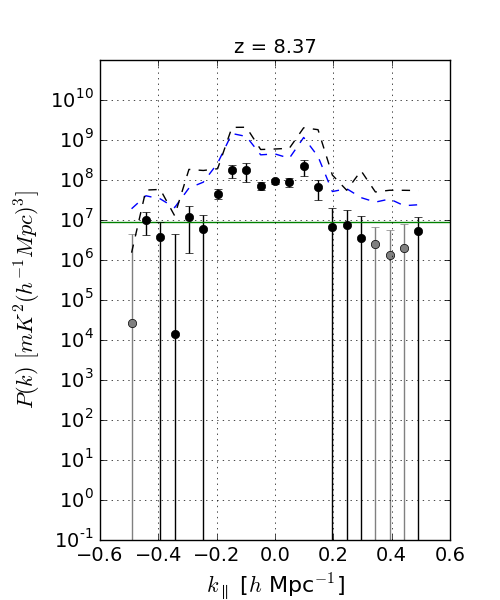
\includegraphics[width=0.4\textwidth]{plots/ps1_data_add.png}
	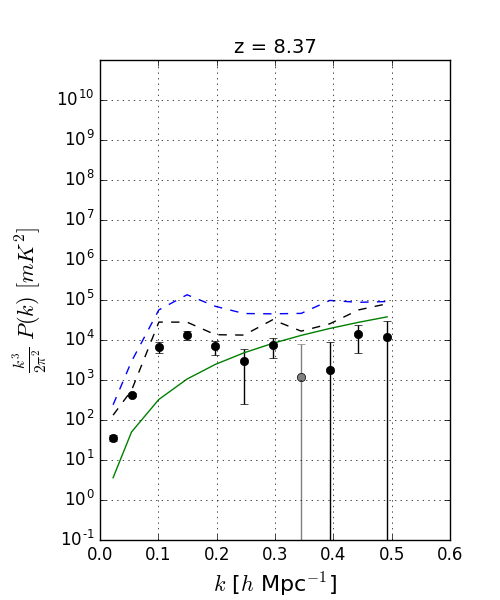
\includegraphics[width=0.4\textwidth]{plots/ps2_data_add.png}
	\caption{Power spectrum of PAPER-64 using $\widehat{\textbf{C}}_{eff}$. Black and gray points correspond to positive and 
negative power spectrum values, respectively, with $2\sigma$ error bars also plotted. The dashed blue line is the unweighted 
power spectrum ($2\sigma$ upper limit). The solid green line is the theoretical $2\sigma$ noise level prediction based on 
observational parameters. This power spectrum result differs from A15 in that it only uses data from one type of baseline ($30$ m 
East/West baselines) instead of three. Major differences from previously published results stem from revisions regarding signal 
loss, bootstrapping, and the theoretical error computation. From this, we quote a best $2\sigma$ upper limit of $(151.0$ mK$)^{2}$ at 
$k=0.34$ $h$Mpc$^{-1}$, a higher limit than A15 by a factor of $\sim7$ in mK \cc{replace with kolopanis limit later}.}
	\label{fig:ps1_data}
\end{figure*}

In this section we have shown three simple ways of regularizing $\widehat{\textbf{C}}$ to minimize signal loss using PAPER-64 
data. There are many other weighting schemes that we leave for consideration in future work. For example, one could estimate 
$\widehat{\textbf{C}}$ using information from different subsets of baselines. For redundant arrays this could mean calculating $
\widehat{\textbf{C}}$ from a different but similar baseline type, such as the $\sim30$ m diagonal PAPER baselines (instead of the 
horizontal E/W ones). Alternately, covariances could be estimated from all other baselines except the two being cross-multiplied 
when forming a power spectrum estimate. This method was used in \citet{parsons_et_al2014} (a similar method was also used in \citet{dillon_et_al2015}) in order to avoid suppressing the 
$21$ cm signal, and it's worth noting that the PAPER-32 results are likely less impacted from the issue of signal loss underestimation 
because of this very reason (however, they are affected by the error estimation issues described in Section \ref{sec:Error}, so 
we also regard those results as suspect and superseded by those of Kolopanis et al., \textit{in prep}).

Another possible way to regularize $\widehat{\textbf{C}}$ is to use information from different ranges of LST. For example, one could 
calculate $\widehat{\textbf{C}}$ with data from LSTs where foregrounds are stronger (earlier or later LSTs than the `foreground-quiet' range used in forming power spectra) --- doing so may yield a better description of the foregrounds that we desire to 
down-weight, especially if residual foreground chromaticity is instrumental in origin and stable in time. Fundamentally, each of these examples are similar in that they rely on a computation of $\widehat{\textbf{C}}$ from 
data that is similar but not exactly the same as the data that is being down-weighted. Ideally this would be effective in down-weighting shared contaminants yet avoid signal loss from over-fitting EoR modes in the power spectrum dataset itself. 

In Section \ref{sec:Sigloss}, we have detailed several aspects of signal loss in PAPER-64: how the loss arises, how it can be estimated, and ways it can be minimized. We again emphasize that these lessons learned about signal loss are largely responsible for shaping our revised analysis of PAPER data. In the remainder of this paper, we will transition to other new aspects of our analysis, framed within the context of error estimation and (non-EoR) bias in PAPER-64.

% SECTION 3 ERROR ESTIMATION ---------------------------------------------------------------------------------

\subsection{PAPER-64: Error Estimation}
\label{sec:Error}

In this section we discuss the ways in which we estimate errors for PAPER-64 power spectra. We first walk through a derivation 
for a theoretical error estimation (of thermal noise) based on observational parameters. Although a theoretical model often 
differs from true errors as explained in Section \ref{sec:ErrorOverview}, it is helpful to understand the ideal case and the factors 
that affect its sensitivity. Additionally, we build on the lessons learned about bootstrapping in Section \ref{sec:ErrorOverview} to 
revise our bootstrapping method as applied to PAPER-64 data in order to compute accurate errors from the data itself.

In particular, we highlight major changes in both our sensitivity calculation and bootstrapping method that differ from the A15 
analysis of PAPER-64. While we do not discuss the changes within the context of PAPER-32, it is worth noting that the power 
spectrum results in \citet{parsons_et_al2014} are affected by the same issues.

\subsubsection{Theoretical Error Estimation}
\label{sec:PSSense}

Re-analysis of the PAPER-64 data included a detailed study using several independently generated noise simulations. What we 
found was that these simulations all agreed but were discrepant with the previous analytic sensitivity calculations. The analytic 
calculation is only an approximation; however, the differences were large enough (factors of $10$ in some cases) to warrant a 
careful investigation. The analytic calculation attempts to combine a large number of pieces of information in an approximate 
way, and when re-considering some of the approximations, we have found there to be large effects. What follows here is an 
accounting of the differences which have been discovered.

The sensitivity prediction (\citealt{parsons_et_al2012a}; \citealt{pober_et_al2013}) for a power spectral analysis of 
interferometric $21$ cm data, in temperature-units, is:

\begin{equation}
\label{eq:sense}
p(k) = \frac{X^{2}Y \Omega_{eff} T_{sys}^{2}}{\sqrt{2N_{lst}N_{seps}}\,t_{int}N_{days}N_{bls}N_{pols}}.
\end{equation}
We will now explain each factor in Equation \eqref{eq:sense} and highlight key differences from the numbers used in A15.

\begin{itemize}
\item $X^{2}Y$: Conversion factors from observing coordinates (angles on the sky and frequency) to cosmological coordinates (co-moving 
distances). For $z=8.4$, $X^{2}Y = 5 \times 10^{11} h^{-3}$ Mpc$^{3}$ str$^{-1}$ GHz$^{-1}$.
\item $\Omega_{eff}$: The effective primary beam area in steradians (\citealt{parsons_et_al2010}; \citealt{pober_et_al2012}). 
The effective beam area changes with the application of a fringe-rate filter, since different parts of the beam are up-weighted and down-weighted. Using numbers from Table 1 in \citet{parsons_et_al2016}, $\Omega_{eff} = 0.74^{2}/0.24$ for an optimal fringe-rate 
filter. 
\item $T_{sys}$: The system temperature is set by:

\begin{equation}
\label{eq:sys}
T_{sys} = 180\Big(\frac{\nu}{0.18}\Big)^{-2.55} + T_{rcvr},
\end{equation}

where $\nu$ are frequencies in GHz. We use a receiver temperature of $144$ K, yielding $T_{sys} = 431$ K at $150$ MHz. 
This is lower than the $T_{sys}$ of $500$ K used in A15 because of several small miscalculation errors that were 
identified\footnote{For example, there was a missing a square root in going from a variance to a standard deviation.}.
\item $\sqrt{2}$: This factor in the denominator of the sensitivity equation comes from taking the real part of the power spectrum 
estimates after cross-multiplying independent `even' and `odd' visibility measurements (which is done principally to avoid a noise bias). In A15, a factor of $2$ was mistakenly used.
\item $N_{lst}$: The number of LST bins that go into a power spectrum estimation. The sensitivity scales as the square root 
because we integrate incoherently over time. For PAPER-64, $N_{lst} = 8$.
\item $N_{seps}$: The number of baseline separation types averaged incoherently in a final power spectrum estimate. For the 
analysis in this paper, we only use one type of baseline, hence $N_{seps}=1$. The updated limits in Kolopanis et al., \textit{in prep}
use three separation types.
\item $t_{int}$: Length of an independent integration of the data. It is crucial to adapt this number if filtering is applied along the time axis (i.e. a 
fringe-rate filter). We compute the effective integration time of our fringe-rate filtered data by scaling the original integration time $t_{i}$
using the following:
\begin{equation}
t_{int} = t_{i} \frac{\int1 \, df}{\int w^{2}(f) \,df},
\end{equation}
where $t_{i}=43$ seconds, $t_{int}$ is the fringe-rate filtered integration time, $w$ is the fringe-rate profile, and the integral is 
taken over all fringe-rates. For PAPER-64, this number is $t_{int} = 3857$ s. 
\item $N_{days}$: The total number of days of data analyzed. In A15, this number was set to $135$. However, because we 
divide our data in half (to form `even' and `odd' datasets), this number should be reduced by a factor of $2$. Additionally, 
because our LST coverage is not $100\%$ complete (it doesn't overlap for every single day), we compute a more realistic value of 
$N_{days}$ as:
\begin{equation}
 \frac{1}{N_{days}} = \sqrt{\Big\langle\frac{1}{N_{i}^{2}} \Big\rangle_{i}},
 \end{equation}
\noindent where $i$ is over LST (\citealt{jacobs_et_al2015}). For PAPER-64, our revised estimate of $N_{days}$ is $\sim34$ 
days.
\item $N_{bls}$: The number of baselines contributing to the sensitivity of a power spectrum estimate. In A15, this number was 
the total number of $30$ m East/West baselines used in the analysis. However, using the total number of baselines neglects 
the fact that baselines are averaged into groups (see Section \ref{sec:Boot}) for computational speed-up when cross-multiplying data. Our revised estimate for the parameter is:
\begin{equation}
N_{bls} = \frac{N_{bls\_total}}{N_{gps}}\sqrt{N_{gps}^{2}-N_{gps}},
\end{equation}
\noindent where, for the A15 analysis, $N_{gps} = 5$. Each baseline group averages down linearly as the number of baselines 
entering the group ($N_{bls\_total}/N_{gps}$) and then as the square root of the number of cross-multiplied pairs ($\sqrt{N_{gps}^{2} - 
N_{gps}}$). For the revised PAPER-64 analysis with only one baseline separation type, this becomes $N_{bls} \sim 46$ instead 
of $51$. 
\item $N_{pols}$: The number of polarizations averaged together. For the case of Stokes I, $N_{pols}=2$.
\end{itemize}

An additional factor of $\sqrt{2}$ is gained in sensitivity when folding our power spectra into $\Delta^{2}(k)$, due to averaging 
together positive and negative $k$'s. 

Our revised sensitivity estimate for PAPER-64 is shown in comparison with that of A15 in Figure \ref{fig:sense_check}. 
Together, the revised parameters yield a decrease in sensitivity (higher noise floor) by a factor of $\sim5$ in mK$^{2}$. 

\begin{figure}
	\centering
	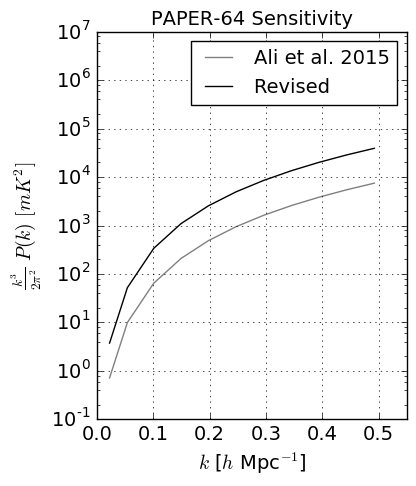
\includegraphics[width=\columnwidth]{plots/sense_check.png}
	\caption{An updated prediction for the noise-level of PAPER-64 data (black) is shown in comparison to previously 
published sensitivity limits (gray). Both sensitivity analyses plotted assume only one baseline type (an additional factor of $
\sqrt{3}$ for three baseline types is needed to match A15 exactly). Major factors that contribute to the discrepancy are $
\Omega_{eff}$, $N_{days}$ and $N_{bls}$, as in Equation \eqref{eq:sense} and described in Section \ref{sec:PSSense}, which when combined decreases our 
sensitivity (higher noise floor) by a factor of $\sim5$ in mK$^{2}$.}
	\label{fig:sense_check}
\end{figure}

To verify our thermal noise prediction, we form power spectra estimates using a pure noise simulation. We create Gaussian 
random noise assuming a constant $T_{rcvr}$ (translated into $T_{sys}$ via Equation \eqref{eq:sys}) but accounting for the true $N_{days}$ as determined 
by LST sampling counts for each time and frequency in the LST-binned data. We convert $T_{sys}$ into a variance statistic 
using:

\begin{equation}
\label{eq:noise}
T_{rms} = \frac{T_{sys}}{\sqrt{\Delta\nu \Delta t N_{days} N_{pols}}},
\end{equation}

\noindent where $\Delta\nu$ is channel spacing, $\Delta t$ is integration time, $N_{days}$ is the number of daily counts for a 
particular time and frequency that went into our LST-binned set, and $N_{pols}$ is the number of polarizations ($2$ for Stokes 
I). This RMS temperature sets the variance of the Gaussian random noise.

Power spectrum results for the noise simulation, which uses our full power spectrum pipeline, are shown in Figure 
\ref{fig:ps_noise}, where the black and gray points represent positive and negative power spectrum values, respectively (with 
$2\sigma$ error bars and weighting matrix $\widehat{\textbf{C}}_{eff}$), the dashed blue line represents the unweighted power 
spectrum, and the solid green line denotes our $2\sigma$ theoretical noise prediction as calculated by Equation 
\eqref{eq:sense}. All three are in agreement, validating our analytical thermal noise calculation. 

\begin{figure*}
	\centering
	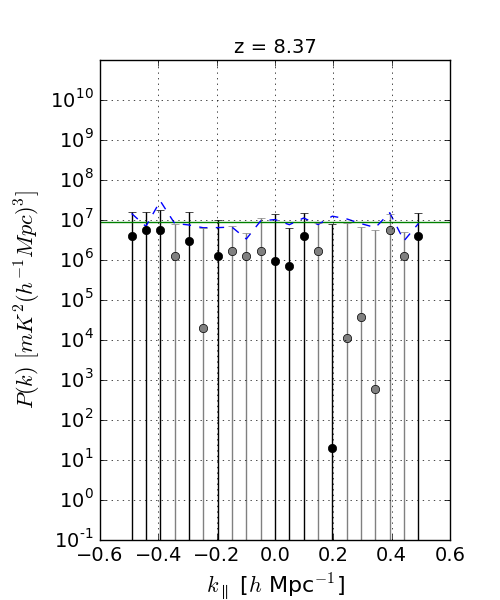
\includegraphics[width=0.4\textwidth]{plots/ps1_noise_add.png}
	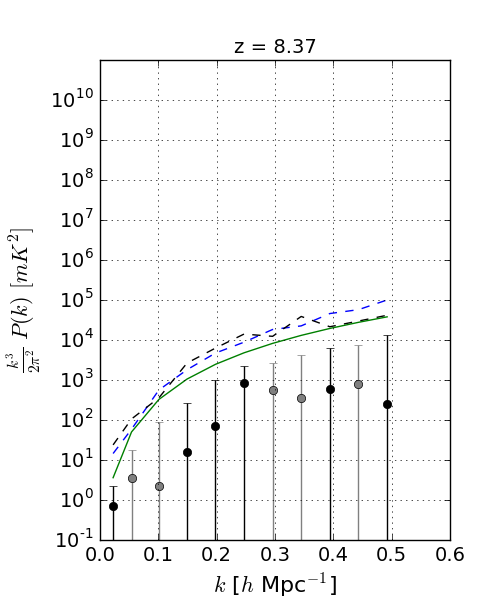
\includegraphics[width=0.4\textwidth]{plots/ps2_noise_add.png}
	\caption{Power spectrum estimate for a noise simulation that mimics the noise level of PAPER-64 data. The weighted 
power spectrum points and their $2\sigma$ errors are show in black and gray (positive and negative values), where we use $
\widehat{\textbf{C}}_{eff}$ to minimize signal loss. The dashed blue line is the unweighted power spectrum (also $2\sigma$ upper 
limit). The solid green line is the theoretical $2\sigma$ noise level prediction as calculated by Equation \eqref{eq:sense}. All three 
estimates agree (the analytic curve should encompass $95\%$ of the points).}
	\label{fig:ps_noise}
\end{figure*}

\subsubsection{Bootstrapping}
\label{sec:Boot}

We bootstrap PAPER-64 power spectra in order to determine confidence intervals for our results. In this section, we highlight 
one major changes in the way we estimate errors since A15, using the lesson we have learned about bootstrapping independent samples.

As discussed in Section \ref{sec:ErrorOverview}, bootstrapping is only a valid way of estimating errors if a dataset is comprised 
of independent samples, or the number of independent samples is well known. The PAPER-64 pipeline outputs $20$ bootstraps (over baselines), each a $2$-dimensional power 
spectrum that is a function of $k$ and time. 

In A15, a second round of bootstrapping occurred over the time axis. A total of $400$ bootstraps were created in this step 
($N_{boot} = 400$), each comprised of randomly selected values sampled with replacement along the time axis. More 
specifically, each of these bootstraps contained the same number of values as the number of time integrations (which, at $\sim$
$700$, greatly exceeds the approximate number of independent samples after fringe-rate filtering).
Medians were then taken of the values in each bootstrap (with the appropriate median correction factor applied). Finally, power 
spectrum limits were computed by taking the mean and standard deviation over all the bootstraps. We emphasize again that in 
this previous analysis, the number of elements sampled per bootstrap greatly 
exceeded the number of independent LST samples, under-estimating errors. A random draw of $700$ 
measurements from this dataset has many repeated values, and the variance between hundreds ($N_{boot}$) of these random 
samples is smaller than the true underlying variance of the data. 

Given our new understanding of the sensitivity of bootstraps to the number of elements sampled, we have removed the second 
bootstrapping step along time entirely and now simply bootstrap over baselines. Power spectrum estimates with this bootstrapping change for fringe-rate filtered noise are shown in Figure 
\ref{fig:data_errors}. The estimates are unweighted in order to disentangle the effects of bootstrapping from signal loss. As 
shown in the figure, when more elements are drawn for each bootstrap than the number of 
independent samples (by over-sampling elements along the time axis), repeated values begin to crop up and the apparent variation between bootstraps drops, resulting in limits (gray) below the predicted noise level (green). Using the revised bootstrapping method, where bootstrapping only occurs over the baseline axis, the errors (black) are shown to agree with the analytic prediction for noise.

\begin{figure}
	\centering
	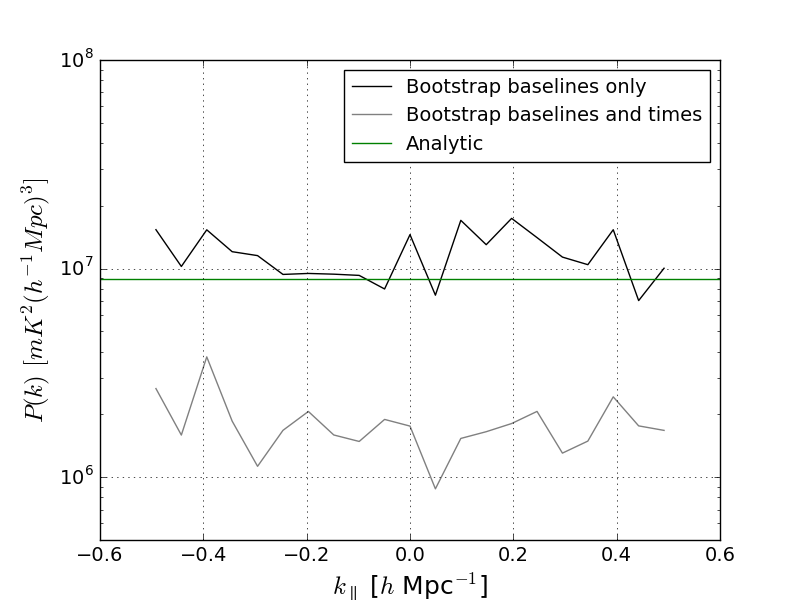
\includegraphics[trim={0.3cm 0cm 0.3cm 0.3cm},width=\columnwidth]{plots/noise_errors.png}
	\caption{$2\sigma$ power spectrum errors (not upper limits) for a noise simulation (computed via Equation \eqref{eq:noise} using PAPER-64 observing parameters) using two different bootstrapping 
methods. The noise is fringe-rate filtered and a weighting matrix of $\textbf{I}$ (unweighted) is used in order to disentangle the 
effects of bootstrapping from signal loss. The bootstrapping method used in A15 in shown in gray, where bootstrapping occurs along both the baseline and time axes. This under-estimates errors by sampling more values than independent ones in the dataset (fringe-rate filtering reduces the number of independent samples along time). We use the method illustrated by the black curve in our updated analysis, where bootstrapping only occurs along the baseline axis. This is shown to agree with the $2\sigma$ analytic prediction for noise (green).}
	\label{fig:data_errors}
\end{figure}

% SECTION 3 BIAS ---------------------------------------------------------------------------------

\subsection{PAPER-64: Bias}
\label{sec:Bias}

In Section \ref{sec:BiasOverview} we highlighted some common sources of bias that can show up as power spectrum 
detections and imitate EoR. We discussed the importance of using jackknife and null tests for instilling confidence in an EoR 
detection, as well as identifying other sources of biases. Here we demonstrate methods used by PAPER-64 to mitigate 
foreground and noise bias and we perform null tests in order to characterize the stability and implications of our results.

\subsubsection{Mitigating Bias}

We briefly discuss one way we mitigate foreground leakage in a power spectrum estimate, and two ways we 
suppress noise biases. These methods are not novel to this analysis but here we frame them in the context of minimizing false 
(non-EoR) detections. 

Tailoring window functions is one way to suppress foreground biases (similar discussions to the following one are in \citet{liu_et_al2014b} and A15). As alluded to in Section \ref{sec:SiglossOverview}, we 
have a choice for the normalization matrix $\textbf{M}$ in Equation \eqref{eq:phat}. For the analysis of PAPER-64 data, we 
compute $\textbf{M}$ using the Fisher matrix $\textbf{F}$, defined as:

\begin{equation}
\textbf{F}_{\alpha\beta} = \frac{1}{2} \text{tr} [\textbf{R}\textbf{Q}^{\alpha}\textbf{R}\textbf{Q}^{\beta} ]
\end{equation}

\noindent where $\textbf{R}$ is the data-weighting matrix and $\alpha$ and $\beta$ are wavebands in $k_{\parallel}$. We take 
the Cholesky decomposition of $\textbf{F}$, decomposing it into two lower triangular matrices (which is possible since $\textbf{F}$ is Hermitian):

\begin{equation}
\textbf{F} = \textbf{LL}^{\dagger}.
\end{equation}

\noindent Next, we construct $\textbf{M}$:

\begin{equation}
\textbf{M} = \textbf{DL}^{-1}
\end{equation}

\noindent where $\textbf{D}$ is a diagonal matrix. In doing so, our window function, defined as $\textbf{W} = \textbf{MF}$, 
becomes:

\begin{equation}
\textbf{W} = \textbf{DL}^{\dagger}.
\end{equation}

\noindent Because of the nature of the lower triangular matrix, this window function has the property of preventing the leakage 
of foreground power from low $k$ to high $k$ modes. Specifically, we order the elements in $\textbf{F}$ in such a way so that 
power can leak from high $k$ modes to low $k$ modes, but not vice versa. Since most foreground power shows up at low 
$k$'s, this method ensures a window function that retains clean, noise-dominated measurements while minimizing the 
contamination of foreground bias. This tailored window function was used in the A15 analysis, however for this paper, we use $\textbf{M} \propto \textbf{I}$ for simplicity.

In addition to mitigating foreground bias at high $k$'s, two other sources of bias that we actively suppress in the PAPER-64 
analysis are noise bias associated with the squaring of thermal noise and noise bias from crosstalk. In order to avoid the 
former, we filter out certain cross-multiplications when forming $\widehat{q}$ in Equation \eqref{eq:qhat}. Namely, the PAPER-64 
dataset is divided into two halves: even julian dates and odd julian dates. Our data vectors are then $\textbf{x}_{even, 1}$ for 
the `even' dataset and baseline group $1$, $\textbf{x}_{odd, 1}$ for the `odd' dataset and baseline group $1$, etc. We only form 
$\widehat{q}$ when the two copies of $\textbf{x}$ come from different groups and baselines, never multiplying `even' with `even', for 
example, in order to prevent the squaring of the same thermal noise. We recognize that this method results in a hit to our sensitivity. Sensitivity can be gained, for example, by only dividing up the dataset once (either along time or baselines), or by creating more groups (more cross-multiplications), but in this paper we only attempt to revise the A15 analysis (which uses the same groupings), not produce the most sensitive limits of PAPER-64.

To mitigate crosstalk bias, which appears as a static bias in time, we apply a fringe-rate filter that suppresses fringe-rates of 
zero. Figure \ref{fig:frp} shows that the filter response is zero for such static signals. The effect of filtering out zero fringe-rates 
on power spectrum results is shown in A15. Most notably, power spectrum detections exist at all $k$'s without crosstalk 
removal and these are detections that, depending on the power spectrum level, could be mistaken for EoR. 

\subsubsection{Jackknife Tests}

The highest sensitivity power spectrum result for PAPER-64 using the updated analysis presented in this paper, shown in 
Figure \ref{fig:ps1_data}, has positive biases at low $k$ values. As discussed in Section \ref{sec:BiasTypes}, these detections 
are most likely attributable to foreground leakage. Here we demonstrate three null tests performed on PAPER-64 data that verify 
that the positive detections are indeed due to foreground variation and not attributable to EoR.

The three null test results are shown in Figure \ref{fig:null}, with each test described as the following:

\begin{itemize}
\item Original Data (black): This is identical to the unweighted, revised PAPER-64 power spectrum in Figure \ref{fig:ps1_data} (one baseline type only) with weighting matrix $\textbf{I}$. There are clear detections at 
low $k$'s.
\item Even/Odd (blue): We split our dataset into even (\textbf{e}) and odd (\textbf{o}) days. We then form the following two datasets: $\textbf{x}_{1} = \textbf{e} + \textbf{o}$ and $\textbf{x}_{2} = 
\textbf{e} - \textbf{o}$. We form datasets in this way to ensure that we use the full sensitivity of our data. When cross-multiplied, we obtain:
\begin{equation}
\textbf{x}_{1}\textbf{x}_{2}^{\dagger} = \textbf{ee}^{\dagger} - \textbf{eo}^{\dagger} + \textbf{oe}^{\dagger} - \textbf{oo}^{\dagger}
\end{equation}
If the same sky signal is in both the even and odd datasets, we expect it to cancel out.
\item Baselines (green): We split our dataset into two halves, where each contains half of the total baselines used in the 
analysis. Again, we form $\textbf{x}_{1} = \textbf{b}_{1} + \textbf{b}_{2}$ and $\textbf{x}_{2} = \textbf{b}_{1} - \textbf{b}_{2}$, where $\textbf{b}_{1}$ is the first baseline 
group and $\textbf{b}_{2}$ is the second baseline group.
\item LST (magenta): We split our dataset into two halves based on LST, namely $\textbf{t}_{1}$ (LSTs 0.5-4.6 hours) and $\textbf{t}_{2}$ (LSTs 
4.6-8.6 hours). We form our two datasets as $\textbf{x}_{1} = \textbf{t}_{1} + \textbf{t}_{2}$ and $\textbf{x}_{2} = \textbf{t}_{1} -\textbf{t}_{2}$.
\end{itemize}

\begin{figure*}
	\centering
	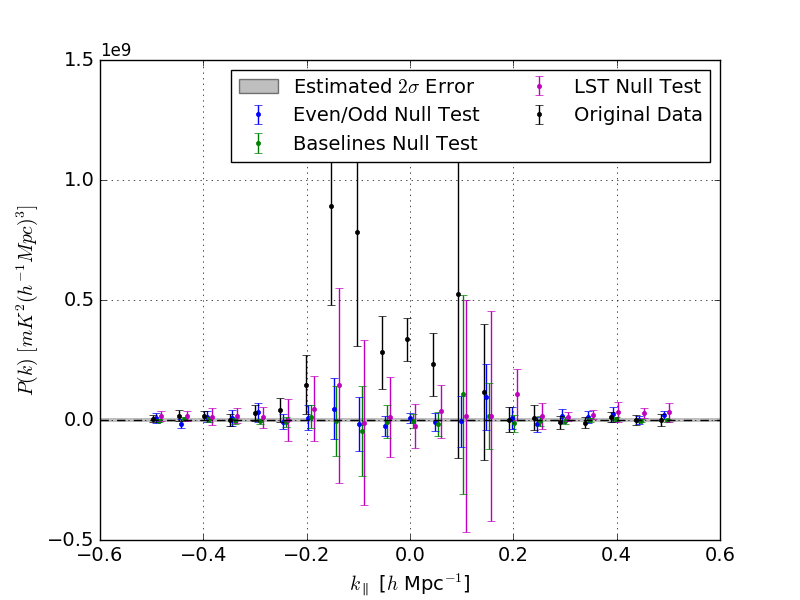
\includegraphics[width=1\textwidth]{plots/null.png}
	\caption{Results for three null tests compared to the PAPER-64 unweighted revised power spectrum (black) and analytically estimated 
$2\sigma$ errors (gray shaded region). For each, we take a jackknife along a different axis of the dataset - along julian days (separating 
even and odd days; blue), along baselines (green), and along LST (magenta). We expect the sky signal to disappear for a `passing' null test (for all error bars to be contained to within the gray shaded region).
We find that none of the null tests performed pass, and that the dominant source of the biases in our power spectrum are likely caused by variation of foregrounds in LST (due to the magenta result being the most inconsistent with noise)}
	\label{fig:null}
\end{figure*}

Investigating Figure \ref{fig:null}, we find that none of the null tests are fully consistent with noise; we would expect the null tests' error bars to be contained within the gray shaded region (theoretical error) for a `passable' test. We note, however, that the error bars for the baselines test (green) and even/odd test (blue) are smaller than those of the LST test (magenta). 

%We note that the error bars for the baselines test (green) are especially small --- this is because the signal is effectively cancelled out prior to cross-multiplication (when forming baseline groups). 

This suggests that the primary systematic driving our power spectrum points and errors to be outside the 
estimated error region is LST-dependent, and therefore likely to be residual foregrounds. In other words, the fact that many magenta power spectrum points are outside the estimated error region implies that $t_{1}$ and 
$t_{2}$ differ by an amount greater than thermal noise and they do not effectively cancel out the sky signal during cross-multiplication. While residual foregrounds are the primary cause for power spectrum results above the theoretical noise (as in Figure \ref{fig:ps1_data}), other unexplained variations exist which are present in all the null tests. These variations could be attributable to... \cc{fill in}

We do not investigate the detailed nature of the residual foregrounds in this paper, though one could imagine performing many 
similar null tests with a sliding window of $t_{1}$'s and $t_{2}$'s. This would illuminate the particular LST range that introduces 
the foreground bias (or whether the bias is constant in LST), and could potentially be traced to an individual bright radio source. 
This type of detailed analysis will be critical at EoR sensitivities; however, for our current analysis we are not surprised that the main source of
bias we see comes from foregrounds in regions where we expect leakage.

% CONCLUSION ---------------------------------------------------------------------------------

\section{Conclusion}
\label{sec:Con}

Although current $21$ cm published power spectrum upper limits lie several orders of magnitude above predicted EoR levels, 
ongoing analyses of deeper sensitivity datasets from PAPER, MWA, and LOFAR, as well as next generation instruments like 
HERA, are expected to continue to push towards EoR sensitivities. As the field progresses towards a detection, we have shown 
that it is crucial for future analyses to have a rigorous understanding of signal loss in an analysis pipeline, be able to accurately 
and robustly calculate both power spectrum and theoretical errors, and consistently undergo a comprehensive set of jackknife 
and null tests.

In particular, in this paper we have investigated the subtleties and tradeoffs of common $21$ cm power spectrum techniques on 
signal loss, error estimation, and bias, which can be summarized as follows:

\begin{itemize}
\item Substantial signal loss can result when weighting data using empirically estimated covariances (Section 
\ref{sec:SiglossOverview}). Loss of the $21$ cm signal is especially significant the fewer number of independent modes that
exist in the data. Hence, there exists a trade-off between sensitivity driven 
time-averaging techniques such as fringe-rate filtering and signal loss when using empirically estimated covariances. 
\item Signal injection and recovery simulations can be used to quantify signal loss (Section \ref{sec:Sigloss}). However, a 
signal-only simulation (i.e. comparing an unweighted vs. weighted power spectrum of EoR only) can underestimate loss by 
failing to account for correlations between the data and signal (Section \ref{sec:Illustration}).
\item Errors that are estimated via bootstrapping can be underestimated if samples in the dataset are significantly correlated 
(Section \ref{sec:ErrorOverview}). If the number of independent samples in a dataset is well-determined, bootstrapping is a 
simple and accurate way of estimating errors.
\item Meaningful null tests are vital to validate an EoR detection (Section \ref{sec:JackknifeOverview}). Similarly, performing 
jackknife tests along multiple axes of a dataset is necessary for confidence in an EoR detection and can also be used to tease 
out systematics.
\end{itemize}

As a consequence of our investigations, we have also revised power spectrum results from PAPER-64. For an analysis of only 
one baseline type, we quote a new $2\sigma$ upper limit of $(151.0$ mK$)^{2}$ at $k=0.34$ $h$Mpc$^{-1}$, a higher limit than 
A15 by a factor of $\sim7$ in mK \cc{replace with kolopanis limit later}. The reasons for a previously underestimated limit and 
ways in which our new analysis differs can be summarized by the following:

\begin{itemize}
\item Signal loss, previously found to be $<2\%$ in A15, was under-estimated by a factor of $\sim$$1000$ for inverse 
covariance weighting. For our new analysis, we use a regularized covariance weighting method to minimize loss (Section 
\ref{sec:Weight}). However, because our revised weighting method is not as aggressive as the former, our results are still a 
factor of $\sim7$ in mK higher than previous limits. Under-estimated signal loss therefore represents the bulk of our revision. We 
note that PAPER's analysis is not the first to under-estimate loss; results from the GMRT (\citealt{paciga_et_al2013}) were also 
revised from new signal loss calculations associated with their singular value decomposition foreground filter.
\item Power spectrum errors, originally computed by bootstrapping, were under-estimated by a factor of $\sim$$1.4$ in mK due to oversampling data whose effective number of independent samples was reduced from fringe-rate filtering (Section \ref{sec:Boot}). 
\item Several factors used in an analytic expression to predict the noise-level in PAPER-64 data were revised, yielding a 
decrease in predicted sensitivity level by a factor of $\sim$$2$ in mK (Section \ref{sec:PSSense}). We have verified our revised 
prediction extensively using pure noise simulations. We note that our sensitivity prediction is revised by a factor less than our 
power spectrum result, implying that if taken at face value, the theoretical prediction for noise in A15 was too high for its data 
points.
\end{itemize}

The future of $21$ cm cosmology is exciting, as new experiments have sensitivities that expect to reach and surpass EoR levels, improved 
foreground mitigation/removal strategies are being developed, and simulations are being designed to better understand 
instruments. On the power spectrum analysis side, robust signal loss simulations, precise error calculations, and 
comprehensive jackknife tests will play critical roles in accurate $21$ cm results. With strong foundations being established now, it is safe to say that we can expect to learn much about reionization and our early Universe in the coming years.


% ACKNOWLEDGEMENTS ---------------------------------------------------------------------------------

\section{Acknowledgements}
CC would like to acknowledge the UC Berkeley Chancellor's Fellowship, National Science Foundation Graduate Research 
Fellowship (Division of Graduate Education award 1106400), and thank Eric Switzer for helpful discussions. PAPER and HERA 
are supported by grants from the National Science Foundation (awards 1440343, and 1636646). ARP, DCJ, and JEA would 
also like to acknowledge NSF support (awards 1352519, 1401708, and 1455151, respectively). SAK is supported by the University of Pennsylvania School of Arts and Sciences Dissertation Completion Fellowship. JSD acknowledges NSF AAPF
award 1701536. We graciously thank SKA-SA for site infrastructure and observing support.
\label{sec:Ack}

% APPENDIX ---------------------------------------------------------------------------------

\appendix
\section{A toy model for signal loss}
\label{sec:sigloss_appendix}

In this Appendix, we examine a toy model for signal loss. Our goal is to derive an analytic formula for power spectrum signal loss. We will also show that in general, signal loss appears as a multiplicative bias on one's power spectrum estimate.

The minimum-variance quadratic estimator $\widehat{p}_\alpha$ for the $\alpha$th bandpower of the power spectrum is given by 
\begin{equation}
\widehat{p}_\alpha = \frac{1} {2 \F_{\alpha \alpha} }\x^t \C^{-1} \Q^{\alpha} \C^{-1} \x,
\end{equation}
where
\begin{equation}
F_{\alpha \alpha} \equiv \frac{1}{2} \textrm{tr} \left( \C^{-1} \Q^\alpha \C^{-1} \Q^\alpha \right)
\end{equation}
is the $\alpha$th diagonal element of the Fisher matrix (for this section only, with no loss of generality, we assume that the data $\textbf{x}$ are real). In our case, however, we do not have \emph{a priori} knowledge of the covariance matrix. Thus, we replace $\C$ with $\Chat$, its data-derived approximation. Our estimator then becomes
\begin{equation}
\label{eq:phatloss}
\widehat{p}_\alpha^\textrm{loss} = \frac{1} {2 \widehat{\F}_{\alpha \alpha} }\x^t \Chat^{-1} \Q^{\alpha} \Chat^{-1} \x,
\end{equation}
where
\begin{equation}
\widehat{F}_{\alpha \alpha} \equiv \frac{1}{2} \textrm{tr} \left( \Chat^{-1} \Q^\alpha \Chat^{-1} \Q^\alpha \right),
\end{equation}
with the label ``loss" to foreshadow the fact that this will be an estimator with signal loss (i.e., a multiplicative bias of less than unity). We will now provide an explicit demonstration of this by modeling the estimated covariance as
\begin{equation}
\label{eq:ChatDef}
\Chat = (1-\eta) \C + \eta \x \x^t,
\end{equation}
where $\eta$ is a parameter quantifying our success at estimating the true covariance matrix. If $\eta = 0$, our covariance estimate has perfectly modeled the true covariance and $\Chat = \C$. On the other hand, if $\eta =1$, then our covariance estimate is based purely on the one realization of the covariance that is our actual data, and we would expect a high level of overfitting and signal loss.

Our strategy for computing the signal loss will be to insert Equation \eqref{eq:ChatDef} into Equation \eqref{eq:phatloss} and to express the resulting estimator $\widehat{p}_\alpha^\textrm{loss}$ in terms of $\widehat{p}_\alpha$. We begin by expressing $\Chat^{-1}$ in terms of $\C^{-1}$ using the Woodbury identity so that
\begin{equation}
\Chat^{-1} = \frac{\C^{-1}}{1-\eta} \left[ \I - \frac{\eta \x \x^t \C^{-1}}{1+ \eta (g-1)}\right],
\end{equation}
where we have defined $g \equiv \x^t \C^{-1} \x$. Inserting this into our Fisher estimate we have
\begin{equation}
\widehat{F}_{\alpha \alpha} = \frac{F_{\alpha \alpha}}{(1-\eta)^2} \left[ 1 -\frac{\eta }{1+ \eta (g-1)} \frac{h_{\alpha \alpha}}{F_{\alpha \alpha}} + \frac{1}{2} \left( \frac{\eta }{1+ \eta (g-1)} \right)^2 \frac{h_\alpha^2}{F_{\alpha \alpha}}\right],
\end{equation}
where $h_\alpha \equiv \x^t \C^{-1} \Q^\alpha \C^{-1} \x $ and $h_{\alpha \alpha} \equiv \x^t \C^{-1} \Q^\alpha \C^{-1} \Q^\alpha \C^{-1}\x $. Note that $g$, $h_\alpha$, and $h_{\alpha \alpha}$ are all random variables, since they depend on $\x$. Inserting these expressions into our estimator gives
\begin{equation}
\label{eq:phatlossexpanded}
\widehat{p}_\alpha^\textrm{loss} = \frac{1}{2} \frac{h_\alpha}{F_{\alpha \alpha}} \left[ 1 - \frac{\eta g}{1+ \eta (g-1)}\right]^2  \left[ 1 -\frac{\eta }{1+ \eta (g-1)} \frac{h_{\alpha \alpha}}{F_{\alpha \alpha}} + \frac{1}{2} \left( \frac{\eta }{1+ \eta (g-1)} \right)^2 \frac{h_\alpha^2}{F_{\alpha \alpha}}\right]^{-1}.
\end{equation}
Both for the purposes of analytical tractability and to provide intuition, we expand this expression to leading 
order in $\eta$. This approximates the limiting case where the covariance $\Chat$ is close to the ideal and the 
lossy covariance is a small perturbation.  The result is
\begin{equation}
\widehat{p}_\alpha^\textrm{loss} \approx \frac{1}{2} \frac{h_\alpha}{F_{\alpha \alpha}} \left[ 1 - \eta \left( g - \frac{h_{\alpha \alpha}}{F_{\alpha \alpha}}\right)\right].
\end{equation}
Taking the ensemble average of both sides and noting that the true power spectrum $p_\alpha$ is equal to $\langle h_\alpha \rangle / 2 F_{\alpha \alpha}$, we obtain
\begin{equation}
\langle \widehat{p}_\alpha^\textrm{loss} \rangle \approx (1- \eta N) p_\alpha + 4 \eta \frac{\rm{tr} (\C^{-1} \Q^\alpha \C^{-1} \Q^\alpha \C^{-1} \Q^\alpha )}{\left[ \rm{tr} (\C^{-1} \Q^\alpha \C^{-1} \Q^\alpha  ) \right]^2} \approx (1- \eta N) p_\alpha,
\end{equation}
where $N$ is the length of $\x$. In the last step we dropped the final term, since it scales as $\eta p_\alpha$ (without the factor of $N$) and is therefore typically small compared to the terms that have been retained. Now, recall that $p_\alpha$ is the \emph{true} power spectrum. This means that it can be decomposed into the sum of the foreground and EoR power spectra, since the foregrounds and EoR are uncorrelated in expectation. This toy example, while not showing the emergence of cross-terms provides a rudimentary motivation for the form of Equation \eqref{eq:LinearPspecSum}. 



\section{Simplified Loss Correction}
\label{sec:Pr_appendix}
One of the main difficulties in defining a signal loss procedure is in the interpretation of the injection procedure `output'. The method described in Section \ref{sec:Sigloss} relies on several assumptions which required justification including the assumption that the number of samples is large enough to treat sample variance as a first order purturbation on the ideal covariance matrix instead of the dominant effect we know it is. \acl{I'm not sure the previous sentence was fair. Again, the appendix is a motivating example. Carina's numerical computations do not rely on the derivation.} However it is possible to ask a slightly different question and with less math still get roughly the same answer.

In the main text we made an estimate of the signal loss effecting only the injected EoR by supposing that the lossy injected signal was the difference between the injected and not injected cases: $P_{out} = \widehat{\textbf{p}}_{r} - \widehat{\textbf{p}}_{x}$. Suppose that we rephrase the question we are asking to: ``At what point would an injected signal be detectable at significant levels?". \acl{Can we justify better why this is the right question? In particular, why is the detection of an injected signal the right thing to look at? After all, the universe doesn't do any signal injections. I think to justify that signal injections are the right thing to consider in the first place, one requires some sort of correspondence between equations analogous to Equation \eqref{eq:Deriv1} and \eqref{eq:Deriv2}.} Instead of disentangling the part of the output power spectrum dominated by the injected signal we can simply use $\widehat{\textbf{p}}_{r}$, the weighted power spectrum of the data plus injected signal.
  
\begin{figure}[tp]
\centering
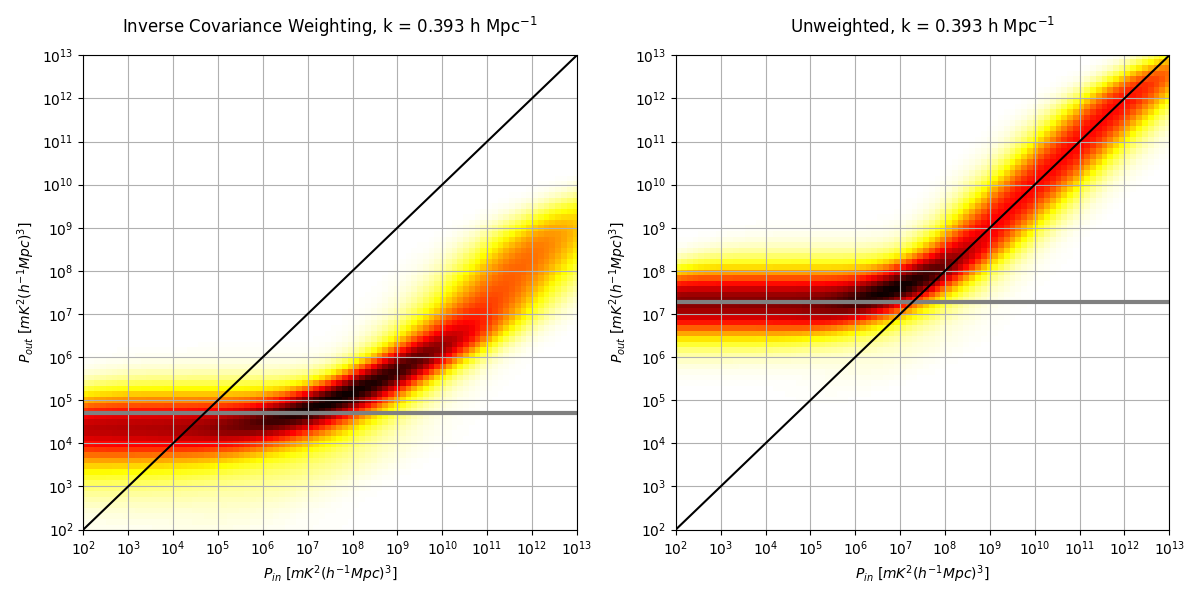
\includegraphics[width=\textwidth]{plots/method2_heatmap_I.png}
\caption{The distribution of $\widehat{\textbf{p}}_{r}$ values for a 
given injection level P$_{in}$. The $\widehat{\textbf{p}}_{r}$ values that are plotted on the y-axis represent the weighted power spectrum of data plus the injected signal. It differs from that of Figure \ref{fig:sigloss_transfercurve} by not subtracting off the power spectrum of data alone (not subtracting off the second term in Equation \eqref{eq:sigloss}). We show kernel density estimations of the power spectrum transfer functions as colored heat-maps for the cases of inverse covariance weighted PAPER-64 data (left) and unweighted data (right). The solid black 
diagonal line marks a perfect unity mapping, and the solid gray horizontal line denotes the peak of $\widehat{\textbf{p}}_{x}$, the data distribution. At low injection, $P_{\rm out}$ converges to the data level.
}
\label{fig:Pr_vs_Pin}
\end{figure}  
  
This question is phrased visually in Figure \ref{fig:Pr_vs_Pin}. In the 2D space relating total $\widehat{\textbf{p}}_r$ to injected $P_{\rm in}$, very small injected levels begin at the level equivalent of no injection (i.e. data only) and very large levels are dominated by the injected signal. It is the transition zone, where the injected signal amplitude is similar to the data level (and thus subject to cross correlations in both the covariance and in the power spectrum calculation) that we search for the point at which an injected signal would be clearly detected.
  
\begin{figure}[tp]
\centering
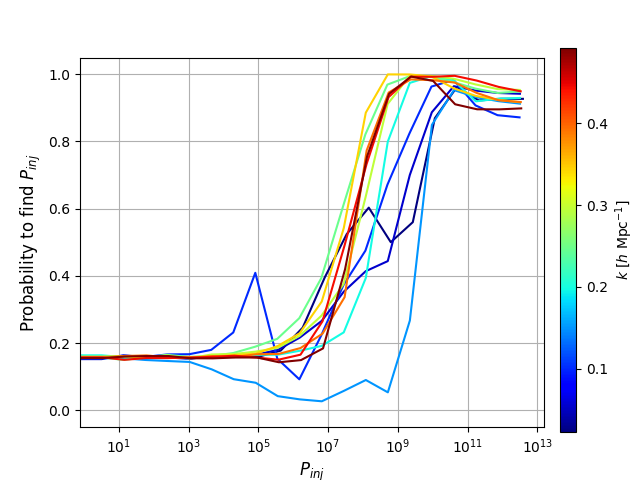
\includegraphics[width=.5\textwidth]{plots/method2_prob_vs_pinj.png}
\caption{The probability that an injected signal of level P$_{inj}$
is observable at a 2$\sigma$ level above the value of $\widehat{\textbf{p}}_{x}$ (data).
The different colors represent different $k$ values. We choose a probability of $95\%$ for our signal loss estimated power spectrum.
\label{fig:Prob_vs_Pin}}
\end{figure}  
  
One difference in this method from the one in the main text is that we are exclusively asking about signals detectable \emph{above} the level of the observed data. Thus it is explicitly limited to placing an upper limit, even if in some $k$-modes one has actual detections above the noise.  This might be seen as more conservative, however, a similar assumption has already been made when choosing to down-weight the data using itself. In such a down-weighting step, one has assumed that significant excess power is associated with a foreground residual. We note that a high SNR detection will require a different method.
  
Formally we can express our test as: ``What is the $P_{\rm in}$ such that the power spectrum of "data + 
injected eor" ($\widehat{p}_{e+x}$) is detectable above the power spectrum of the data itself ($\widehat{p}_x$. 
In other words, what is $e$ such that,
\begin{equation}
\widehat{\textbf{p}}_{e+x} > \widehat{\textbf{p}}_{x},
\end{equation}  
?''  Of course, both sides of this equation are actually a distribution of values associated with data variance and injected model variance. One way to interpret this test for the two distributions is to compute the probability that the two distributions are not (i.e. the null test) the same.  
 \acl{I'm confused a little by this equation. I would've thought that the right thing to do would be to first compute $x_0$, given implicitly by
 \begin{equation}
 \int_{-\infty}^{x_0}\Prob(\widehat{\textbf{p}}_x) dx = \Lambda,
 \end{equation}
 where $\Lambda$ is the appropriate number for $2\sigma$. That tells us what $x$ would be needed for us to thing that it was an outlier result without there being an extra $e$ in the data. Then we ask how often we get such an outlier result by computing
  \begin{equation}
 \int_{x_0}^\infty \Prob(\widehat{\textbf{p}}_{e+x}|P_{e}) dx.
\end{equation}
Is what you've written equivalent to this? Sorry if this is remedial...
 }
 \begin{equation}
\Prob(P_{e})  =  1 -  \int \Prob(\widehat{\textbf{p}}_x) \Prob(\widehat{\textbf{p}}_{e+x}|P_{e}) x
 \end{equation}
 where $\Prob(\widehat{\textbf{p}}_x)$ is the probability of obtaining the power spectrum $\widehat{\textbf{p}}_x$ found via bootstrapping (power spectrum of data only) and $\Prob(\widehat{\textbf{p}}_{e+x}|P_{e})$ is the probability of obtaining the summed power spectrum $\widehat{\textbf{p}}_{x+e}$ given a range of input power levels, as sampled in Figure \ref{fig:Pr_vs_Pin}.  
 
Probability vs. injection level is shown in Figure \ref{fig:Prob_vs_Pin}. At low injection levels the variation between $\textbf{x}$ and $\textbf{(e+x)}$ is such that the null test is ruled out to within $20$\%. This is the level expected from two distributions with $\sim$10 effective samples. 
As the injected signal approaches the level of the data, the probability of null rejection rises steeply.
  
Lastly, this method requires that we choose the probability at which we choose to reject the null hypothesis. As can be seen in Figure \ref{fig:Prob_vs_Pin}, the difference between $80$\% and $90$\% can mean a difference of almost an order of magnitude in the power spectrum level that is ruled out. We can also see that, due to the small number of samples, the probability does not perfectly converge at high injected power levels. Rather than insist on a rejection at the $99$th percent level, we compromise at $95$\%.

The resulting limits for inverse covariance weighted PAPER-64 data (the same data used in Section \ref{sec:Sigloss}, no regularization), using this second signal loss method, are shown in Figure \ref{fig:sigloss_compare} compared with the method used in the main text. Overall the limits show good agreement, with k modes differing by factors of $\sim$$3$.  

\begin{figure}[t]
\centering
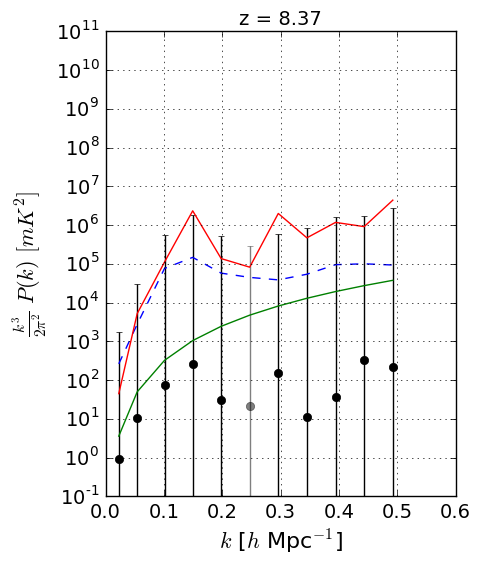
\includegraphics[width=.4\textwidth]{plots/sigloss_method_comparison_95.png}
\caption{A comparison of the signal loss method described in Section \ref{sec:Sigloss}
with the method in this appendix at $95$\% confidence (red curve).
Also shown are the upper limits of the unweighted power spectrum
(blue dashed) and theoretical noise model (green).} 
\label{fig:sigloss_compare} 
\end{figure}

\bibliographystyle{apj}
\bibliography{refs}


\end{document}

